%% This is the ctufit-thesis example file. It is used to produce theses
%% for submission to Czech Technical University, Faculty of Information Technology.
%%
%% Get the newest version from
%% https://gitlab.fit.cvut.cz/theses-templates/FITthesis-LaTeX
%%
%%
%% Copyright 2021, Eliska Sestakova and Ondrej Guth
%%
%% This work may be distributed and/or modified under the
%% conditions of the LaTeX Project Public Licenese, either version 1.3
%% of this license or (at your option) any later version.
%% The latest version of this license is in
%%  https://www.latex-project.org/lppl.txt
%% and version 1.3 or later is part of all distributions of LaTeX
%% version 2005/12/01 or later.
%%
%% This work has the LPPL maintenance status `maintained'.
%%
%% The current maintainer of this work is Ondrej Guth.
%% Contact ondrej.guth@fit.cvut.cz for bug reports.
%% Alternatively, submit bug reports into the tracker at
%% https://gitlab.fit.cvut.cz/theses-templates/FITthesis-LaTeX/issues
%%
%%

%%%%%%%%%%%%%%%%%%%%%%%%%%%%%%%%%%%%%%%%%
% CLASS OPTIONS
% language: czech/english/slovak
% thesis type: bachelor/master/dissertation
% colour: bw for black&white OR no option for default colour scheme
%%%%%%%%%%%%%%%%%%%%%%%%%%%%%%%%%%%%%%%%%
\documentclass[english,master,unicode]{ctufit-thesis}

%%%%%%%%%%%%%%%%%%%%%%%%%%%%%%%%%%
% FILL IN THIS INFORMATION
%%%%%%%%%%%%%%%%%%%%%%%%%%%%%%%%%%
\ctufittitle{Multiple target tracking with external information} % replace with the title of your thesis
\ctufitauthorfull{Bc. Andrey Babushkin} % replace with your full name (first name(s) and then family name(s) / surname(s)) including academic degrees
\ctufitauthorsurnames{Babushkin} % replace with your surname(s) / family name(s)
\ctufitauthorgivennames{Andrey} % replace with your first name(s) / given name(s)
\ctufitsupervisor{doc.\,Ing.\,Kamil Dedecius,\,Ph.D.} % replace with name of your supervisor/advisor (include academic degrees)
\ctufitdepartment{Department of Applied Mathematics} % replace with the department of your defence
\ctufityear{2023} % replace with the year of your defence
\ctufitdeclarationplace{Prague} % replace with the place where you sign the declaration
\ctufitdeclarationdate{\today} % replace with the date of signature of the declaration
\ctufitabstractCZE{Tato práce se zaměřuje na problém sledování více cílů v prostředí s vysokým množstvím rušení a nejistotou ohledně počtu sledovaných objektů pomocí Bayesovské inference. V této práci se hlavně zaměřujeme na populární Gaussian mixture probability hypothesis density (GM-PHD) filtr a představujeme techniku, jak zahrnout dodatečné informace pro případy, kdy senzor nedokáže detekovat sledované objekty z důvodu fyzických nebo prostředkových omezení. Poskytujeme veškeré potřebné teoretické pozadí od základů teorie pravděpodobnosti až po diskusi o různých metodách sledování více cílů a představení rámce Finite Set Statistics (FISST). Dále zahrnujeme rozsáhlé měření výkonnosti a analýzu výsledků, kde ukazujeme, že navržená technika fúze výrazně zlepšuje sledovací výsledky. Nakonec diskutujeme omezení filtru a navrhujeme možné způsoby, jak je překonat.
}
\ctufitabstractENG{The thesis focuses on the multi-target tracking problem in cluttered environments with the uncertainty on the number of targets and using Bayesian inference. In this work, we mainly focus on the popular Gaussian mixture probability hypothesis density (GM-PHD) filter and introduce a technique to include additional information for cases when a sensor fails to detect targets due to environmental or physical limitations. We provide all required theoretical background from the basics of probability theory to the discussion of various multi-target tracking methods and the introduction of the Finite Set Statistics (FISST) framework. We also conclude with an extensive performance measurement and analysis of results, where we demonstrate that the proposed fusion technique significantly improves tracking results. Finally, we discuss the limitations of the filter and propose possible measures to overcome them.
}
\ctufitkeywordsCZE{Bayesovské filtrování, sledování více cílů, náhodné množiny, gaussian mixture probability density filtr, fúze externích informací}
\ctufitkeywordsENG{Bayesian filtering, multi-target tracking, random finite sets, Gaussian Mixture Probability Density filter, external information fusion
}
%%%%%%%%%%%%%%%%%%%%%%%%%%%%%%%%%%
% END FILL IN
%%%%%%%%%%%%%%%%%%%%%%%%%%%%%%%%%%

%%%%%%%%%%%%%%%%%%%%%%%%%%%%%%%%%%
% CUSTOMIZATION of this template
% Skip this part or alter it if you know what you are doing.
%%%%%%%%%%%%%%%%%%%%%%%%%%%%%%%%%%

\RequirePackage{iftex}[2020/03/06]
\iftutex % XeLaTeX and LuaLaTeX
    \RequirePackage{ellipsis}[2020/05/22] %ellipsis workaround for XeLaTeX
\else
    \RequirePackage[utf8]{inputenc}[2018/08/11] %this file encoding
    \RequirePackage{lmodern}[2009/10/30] % vector flavor of Computer Modern font
\fi

% hyperlinks
\RequirePackage[pdfpagelayout=TwoPageRight,colorlinks=false,allcolors=decoration,pdfborder={0 0 0.1}]{hyperref}[2020-05-15]

% uncomment the following to hide all hyperlinks
% \RequirePackage[pdfpagelayout=TwoPageRight,hidelinks]{hyperref}[2020-05-15]

\RequirePackage{pdfpages}[2020/01/28]

\setcounter{secnumdepth}{4} % numbering sections; 4: subsubsection

%%%%%%%%%%%%%%%%%%%%%%%%%%%%%%%%%%
% CUSTOMIZATION of this template END
%%%%%%%%%%%%%%%%%%%%%%%%%%%%%%%%%%


%%%%%%%%%%%%%%%%%%%%%%
% DEMO CONTENTS SETTINGS
% You may choose to modify this part.
%%%%%%%%%%%%%%%%%%%%%%
\usepackage{dirtree}
\usepackage{lipsum,tikz}
\usepackage{csquotes}
\usepackage[style=iso-numeric]{biblatex}
\addbibresource{text/references.bib}
\usepackage{listings} % typesetting of sources
\usepackage{caption}
\usepackage{subcaption}  % subfigures
\usepackage{mathrsfs}  % mathscr
\usepackage{todonotes}  % TODOs that are not later lost
\usepackage{epigraph}  % nice quotes
\usepackage{algorithm}  % algorithms
\usepackage{algpseudocode}  % pseudocode elements
% \usepackage{minted} % typesetting of sources

%theorems, definitions, etc.
\theoremstyle{plain}
\newtheorem{theorem}{Theorem}
\newtheorem{lemma}[theorem]{Lemma}
\newtheorem{corollary}[theorem]{Corollary}
\newtheorem{proposition}[theorem]{Proposition}
\newtheorem{definition}[theorem]{Definition}
\theoremstyle{definition}
\newtheorem{example}[theorem]{Example}
\theoremstyle{remark}
\newtheorem{note}[theorem]{Note}
\newtheorem*{note*}{Note}
\newtheorem{remark}[theorem]{Remark}
\newtheorem*{remark*}{Remark}
\numberwithin{theorem}{chapter}
%theorems, definitions, etc. END
%%%%%%%%%%%%%%%%%%%%%%
% DEMO CONTENTS SETTINGS END
%%%%%%%%%%%%%%%%%%%%%%

\begin{document} 
\frontmatter\frontmatterinit % do not remove these two commands


\includepdf[pages={1-}]{assignment-include.pdf} % replace that file with your thesis assignment provided by study office

\thispagestyle{empty}\cleardoublepage\maketitle % do not remove these three commands

\imprintpage % do not remove this command

\tableofcontents % do not remove this command
%%%%%%%%%%%%%%%%%%%%%%
% list of other contents: figures, tables, code listings, algorithms, etc.
% add/remove commands accordingly
%%%%%%%%%%%%%%%%%%%%%%
\listoffigures % list of figures
\begingroup
\let\clearpage\relax
\listoftables % list of tables
% \lstlistoflistings % list of source code listings generated by the listings package
% \listoflistings % list of source code listings generated by the minted package
\endgroup
%%%%%%%%%%%%%%%%%%%%%%
% list of other contents END
%%%%%%%%%%%%%%%%%%%%%%

\begin{acknowledgmentpage}
	First and foremost, I would like to express my heartfelt gratitude to doc. Ing. Kamil Dedecius, Ph.D. for his unwavering support and guidance throughout the course of this thesis. His invaluable advice, expertise, and continued positive outlook on the world have been a source of inspiration and motivation.

    I would also like to extend my thanks to prof. Ing. Václav Hlaváč, CSc. and Mgr. Radoslav Škoviera, Ph.D. for giving me the opportunity to work as a researcher and for introducing me to the fascinating field of multi-target tracking.

    Furthermore, I wish to express my deepest appreciation to my family and my girlfriend, who provided me with unwavering support during the challenging times and kept me motivated throughout the journey.

    Last, but not least, I express my gratitude and love to my friends Ing. Mykyta Boiko and Ing. Vladyslav Zavirskyy, with whom I started my academic journey when we enrolled in the Bachelor's program together and with whom we have been together throughout the years until the end of our Master's degree.
\end{acknowledgmentpage}

%%%%%%%%%%%%%%%%%%%
% DECLARATION
% FILL IN / MODIFY
%%%%%%%%%%%%%%%%%%%
% INSTRUCTIONS
% ENG: choose one of approved texts of the declaration. DO NOT CREATE YOUR OWN. Find the approved texts at https://courses.fit.cvut.cz/SFE/download/index.html#_documents (document Declaration for FT in English)
% CZE/SLO: Vyberte jedno z fakultou schvalenych prohlaseni. NEVKLADEJTE VLASTNI TEXT. Schvalena prohlaseni najdete zde: https://courses.fit.cvut.cz/SZZ/dokumenty/index.html#_dokumenty (prohlášení do ZP)
\begin{declarationpage}
I hereby declare that the presented thesis is my own work and that I have cited all sources of information in accordance with the Guideline for adhering to ethical principles when elaborating an academic final thesis.

I acknowledge that my thesis is subject to the rights and obligations stipulated by the Act No. 121/2000 Coll., the Copyright Act, as amended, in particular that the Czech Technical University in Prague has the right to conclude a license agreement on the utilization of this thesis as a school work under the provisions of Article 60 (1) of the Act.
\end{declarationpage}
%%%%%%%%%%%%%%%%%%%
% DECLARATION END
%%%%%%%%%%%%%%%%%%%

\printabstractpage % do not remove this command
% %%%%%%%%%%%%%%%%%%%
% SUMMARY
% FILL IN / MODIFY
% OR REMOVE ENTIRELY (upon agreement with your supervisor)
% (appropriate to remove in most theses)
%%%%%%%%%%%%%%%%%%%
\begin{summarypage}
\section*{Summary section}

\lipsum[1][1-8]

\section*{Summary section}

\lipsum[2][1-6]

\section*{Summary section}

\lipsum[3]

\section*{Summary section}

\lipsum[2]

\section*{Summary section}

\lipsum[1][1-8] Lorem lorem lorem.
\end{summarypage}
%%%%%%%%%%%%%%%%%%%
% SUMMARY END
%%%%%%%%%%%%%%%%%%%

\chapter{List of Acronyms}%%%%%%%%%%%%%%%%%%%
% ABBREVIATIONS
% FILL IN / MODIFY
% OR REMOVE ENTIRELY
% List the abbreviations in lexicography order.
%%%%%%%%%%%%%%%%%%%
\chapter{List of Acronyms}

\begin{tabular}{rl}
CV & Constant Velocity \\
EKF & Extended Kalman filter \\
FISST & Finite Set Statistics \\
FoV & Field of view \\
GM & Gaussian mixture \\
HO-MHT & Hypothesis-oriented Multiple Hypothesis Tracker \\
JPDA & Joint Probabilistic Data Association \\
KF & Kalman filter \\
MAP & Maximum a posteriori \\
MHT & Multiple Hypothesis Tracker \\
MLE & Maximum Likelihood Estimator \\
MMSE & Minimum Mean Square Error \\
MTT & Multitarget tracking \\
PDA & Probabilistic Data Association \\
PHD & Probability hypothesis density \\
PPP & Poisson Point Process \\
RFS & Random Finite Set \\
TO-MHT & Track-oriented Multiple Hypothesis Tracker \\
UKF & Unscented Kalman Filter \\
\end{tabular}
%%%%%%%%%%%%%%%%%%%
% ABBREVIATIONS END
%%%%%%%%%%%%%%%%%%%


%%%%%%%%%%%%%%%%%%%
% THE THESIS
% MODIFY ANYTHING BELOW THIS LINE
%%%%%%%%%%%%%%%%%%%

%%%%%%%%%%%%%%%%%%%%%%%%%%%%%%%%%%%%%%%%%%
% Commands
%%%%%%%%%%%%%%%%%%%%%%%%%%%%%%%%%%%%%%%%%%
\newcommand{\varat}[2]{\relax\ifmmode{#1}_{#2}\else ${#1}_{#2}$\fi}
\newcommand{\vecat}[2]{\relax\ifmmode\mathbf{#1}_{#2}\else $\mathbf{#1}_{#2}$\fi}
\newcommand{\svecat}[3]{\relax\ifmmode\vecat{#1}{#2}^{#3}\else $\vecat{#1}{#2}^{#3}$\fi}
\renewcommand{\Pr}[1]{\operatorname{Pr}\{#1\}}

\graphicspath{figures}
\mainmatter\mainmatterinit % do not remove these two commands

%%%%%%%%%%%%%%%%%%%%%%%%%%%%%%%%%%%%%%%%%%
% Introduction
%%%%%%%%%%%%%%%%%%%%%%%%%%%%%%%%%%%%%%%%%%
\addcontentsline{toc}{chapter}{Introduction}\markboth{Introduction}{Introduction}
\setcounter{page}{1}

\chapter*{Introduction}\label{ch:introduction}
    Object tracking is a critical problem in signal processing and computer vision. The primary goal of tracking algorithms is to estimate the states of moving targets based on a sequence of sensor measurements in environments with a high degree of uncertainty. Different domains of the problem require different approaches to target tracking. In this work, we provide an overview of the existing areas of target tracking and introduce the scope of this study.

Tracking algorithms can be categorized based on the number of targets they track, whether it is a fixed or known number of targets, or a variable and unknown number of targets. When the number of targets in the tracking area is greater than one, we refer to it as multi-target tracking (MTT). Object tracking is widely used in various fields, including robotics, autonomous vehicles, surveillance, and medical imaging. With the recent emergence of deep learning algorithms, there has been renewed interest in MTT, and many new deep learning-based approaches have been proposed. However, the learned model's predictive power is questionable, as these approaches estimate the internal object dynamics using complex non-linear models, while the Bayesian approach assumes fixed known model that are specified manually according to some prior knowledge, for instance, physical laws. In this study, we focus on MTT using Bayesian inference, the statistical approach based on recursive updates of the target posterior distribution using a set of measurements.

Bayesian algorithms are classified based on the results they achieve \cite[11]{sarkkaBayesianFilteringSmoothing2013}. The first type of algorithms is Bayesian smoothers, which remove the noise of states based on past and future measurements, i.e., they smooth the signal. The other type is Bayesian predictors, which predict the future state of a target more than one step ahead based on past measurements. The last type is Bayesian filters, which predict the current state of a target based on measurements up to the moment of the predicted state. The Kalman filter, the fundamental algorithm for many modern and sophisticated tracking methods, is an example of Bayesian filters. This study focuses on Bayesian filters, and we cover the Kalman filter in detail.

Algorithms can also be separated based on the type of sensor and measurements used. There are several sets of algorithms available to address specific problems depending on the sensors used. For instance, point object tracking is used when the sensor generates one measurement per object, such as a radar or a camera with an object recognition algorithm. When lidars are used, one target generates a set of measurements, and this is referred to as extended object tracking \cite{granstromExtendedObjectTracking2017}. In surveillance, especially when tracking people, group object tracking algorithms are used to estimate groups of individuals rather than every individual separately \cite{salmondGroupExtendedObject1999}. Additionally, tracking with multipath propagation refers to scenarios where a sensor receives more than one detection caused by the multipath phenomenon or multiple reflections from surrounding objects of the same signal \cite{bar-shalomTrackingLowElevation1994}. Finally, tracking with unresolved targets occurs when several targets produce only one measurement \cite{angleMultipleTargetTracking2021}. In this study, we focus on point object tracking, assuming that one target produces at most one measurement, and each measurement can be generated by at most one target.

This study aims to enhance the performance of the Gaussian Mixture probability hypothesis density (GM-PHD) filter, a popular Bayesian filter for multi-target tracking (MTT), by proposing a novel approach to incorporate external information. Specifically, we provide a detailed description of the GM-PHD filter and its internals, and demonstrate through an example how the filter may fail under environmental limitations. We then introduce our proposed method for integrating external information and analyze its impact on the filter's performance. Finally, we evaluate the filter's strengths and weaknesses in various scenarios and discuss the significance of our contribution in improving the accuracy and robustness of the GM-PHD filter for MTT.

    \section*{Structure}\label{sec:structure}
        The thesis is structured as follows. Chapter 1 provides the theoretical background necessary for understanding the rest of the thesis, including the introduction of probability theory and probability distributions and the Bayes' rule. Next, we present the Bayesian inference framework, which is the basis for the general Bayes filter, a recursive algorithm for state estimation. Finally, we present the concepts of state-space models and the Kalman filter.

Chapter 2 is dedicated to multi-target tracking. It starts with an overview of target tracking methods, followed by an introduction to Random Finite Sets (RFS). The chapter then describes the PHD filter and the PHD function. Next, we give a PHD filter formal definition, and then observe the Gaussian Mixture PHD filter. The chapter concludes with a discussion of track maintenance, the GM-PHD recursion, and ends with the framework for external information fusion.

Chapter 3 describes the implementation and testing methodology of the GM-PHD filter. We then introduce several metrics that are used to measure the performance of multi-target tracking algorithms, then we describe four testing scenarios. The final section on parameters testing and methodology explains how the tests were conducted and how the results were analyzed.

Chapter 4 analyzes the results of the tests conducted in Chapter 3. This chapter includes sections on test results for each scenario and a discussion of the results, where a comprehensive analysis of the filter strengths and weaknesses is provided.

The final Chapter 5 concludes this work by summarizing the main contributions of the thesis and highlighting areas for future research.


%%%%%%%%%%%%%%%%%%%%%%%%%%%%%%%%%%%%%%%%%%
% Theoretical background
%%%%%%%%%%%%%%%%%%%%%%%%%%%%%%%%%%%%%%%%%%
\chapter{Theoretical background}\label{ch:theory}
    The field of target tracking, both single and multiple, rely on mathematical concepts and methods based on probability theory. In this chapter, we provide an introduction to key concepts of probability and inference. We start by reviewing the basics of probability theory, including random variables, probability distributions with examples of the most important ones for multi-target tracking, and the Bayes' theorem. Then, we describe the concept of state-space models, a powerful framework that allows to describe dynamic system evolving in time. Then, we apply these concepts with a Bayes filter, a general method for recursive estimation the state of a dynamic system using measurements obtained from a sensor over time. Finally, we define and prove two important in tracking theorems, and use these theorems to derive the Kalman filter, and important and widely used framework that provides an optimal state estimate of a linear system in the presence of Gaussian noise. The theoretical foundations in this chapter serve as a basis for the next chapter, which covers more sophisticated algorithms for tracking multiple targets in noisy environments.

    \section{Probability theory foundations}\label{sec:prob-foundations}
        When we are dealing with probability of an event, we assume that there is a possibility
of that event occurring and we measure it using a number between 0 and 1 or a percentage
between 0\% and 100\%. In other words, we use the probability theory framework to assign
numerical values to arbitrary events. This section covers several fundamental concepts of
probability theory, which serve as the basis for this work.

The \textit{event}, which we formally denote as $E$, comes from some space of all possible
events, the \textit{outcome space} $\Omega$. We also denote the \textit{probability} of the
event $E$ as $\Pr{E}$. This probability is a real non-negative number,
that is $\Pr{E} \in \mathbb{R}, \Pr{E} \geq 0$. The outcome
space covers all possible events, that is $\Pr{\Omega} = 1$. It then follows
that the probability of disjoint events from the outcome space $\Omega$ is the sum of
probabilities of these events, that is for
$E_1, \ldots, E_n \in \Omega, \Pr{\bigcup_{i=1}^n E_i} = \sum_{i=1}^n \Pr{E_i}$.

We have defined three main axioms of probability theory. In addition to these axioms, several
crucial concepts illustrate the relationship between events. Given two events, $E_1$ and $E_2$,
the \textit{conditional probability} of $E_1$ given $E_2$ is defined as

$$
\Pr{E_1 \mid E_2} = \frac{\Pr{E_1 \cap E_2}}{\Pr{E_2}}.
$$

If the events are \textit{independent} of each other, the probability of them occurring
simultaneously is given by

$$
\Pr{E_1 \cap E_2} = \Pr{E_1}\Pr{E_2}.
$$

These relationships allow us to define the \textit{law of total probability}
\cite[31]{zwillingerCRCStandardProbability2000}, which is a key component of Bayes' rule.
Let $A$ be an event, $A \int \Omega$, and $\{B_n : n = 1, 2, \ldots\}$ be a countable
partition of the space $\Omega$. Then, we have:

$$
\Pr{A} = \sum_n \Pr{A \mid B_n} \Pr{B_n}.
$$

Now, we can deduce the following rule:

\begin{definition}[Bayes' rule]
Let $A$ and $B$ be two events from the outcome space $\Omega$. Then the following applies:

$$
\Pr{A \mid B} = \frac{\Pr{B \mid A}}{\Pr{B}}
    = \frac{\Pr{B \mid A}}{\sum_n \Pr{B \mid A_n}\Pr{A_n}}.
$$
\end{definition}

Bayes' rule plays a crucial role in Bayesian inference and serves as the basis for
Bayesian filters, including the PHD filter.

        \subsection{Probability distributions}\label{sec:prob-distributions}
            Events and their probabilities are not sufficient for our purposes;
we need a framework that allows us to obtain a formal, general description of a set
of events from some outcome space. Specifically, we need an abstraction around events,
which is some function that maps the outcome space $\Omega$ to some other space,
typically $\mathbb{R}$ (but not necessarily). This abstraction is called a
\textit{random variable} and one outcome of it is called a \textit{realization}.

\begin{definition}[Random variable and its realization]
    Let $\Omega$ be a set of possible events, $\omega \in \Omega$ is some event,
    and $\mathbb{O}$ be another space. A function $X: \Omega \rightarrow \mathbb{O}$
    is called a random variable and $x = X(\omega)$ is called a realization of $X$.
\end{definition}

The above definition provides a general framework for understanding random variables.
However, for the purposes of Bayesian statistics, we will simplify the discussion by
focusing on scalar, continuous-valued random variables, represented
by $\mathbb{O} = \mathbb{R}$. In practice, it is often impractical to calculate the
probability of every possible event from the outcome space $\Omega$, especially for
continuous random variables with uncountably infinite outcomes. Instead, it may suffice
to work with intervals on the outcome space and their probabilities. We call such a
probability distribution a \textit{cumulative distribution function (cdf)} of $X$,
and the first-order derivative of the cdf is called a \textit{probability density
function (pdf)}.\footnote{
    For discrete random variables, the corresponding distribution function is
    called a \textit{probability mass function (pmf)}.
}

\begin{definition}[Cumulative distribution function (cdf)]
    Given a scalar real-valued random variable $X \in \mathbb{R}$ and $x$ as a
    realization of $X$, we define the probability $\Pr{X \in (-\infty, x)} = \Pr{X < x}$
    as the cumulative distribution function of random variable $X$ and denote it as $P(x)$.
\end{definition}

\begin{definition}[Probability density function (pdf)]
    The probability density function $p(x)$ of a scalar real-valued random variable $X$
    is defined as:
    $$
    p(x) = \frac{\partial P(x)}{\partial x}.
    $$
\end{definition}

Probability distributions are fundamental in Bayesian statistics and provide a way
to model and analyze the behavior of random variables. In the next section,
we will discuss some common probability distributions used in Bayesian filters,
including the Gaussian distribution and the Poisson distribution.

Probability distributions are fundamental in Bayesian statistics and provide a way
to model and analyze the behavior of random variables. Cdfs and pdfs (as well as pmfs
for discrete cases) are used to specify the probability distribution of a random
variable, providing a formal description of the relationship
between events and probabilities. In addition to this formal description, we also
need to know several statistical properties of probability distributions to fully
understand their behavior. Two main properties of probability distributions are
the expected value, $E[X]$, and the variance, $\operatorname{Var}[X]$:

$$
\begin{aligned}
E[X]&=\int_{-\infty}^{\infty} x p(x) d x, \\
\operatorname{Var}[X]
    &= E\left[(X-E[X])^2\right]
    =\int_{-\infty}^{\infty}(x-E[X])^2 p(x) d x.
\end{aligned}
$$

The expected value, or the first moment, represents the most probable value of
a random variable. The variance, or the second central moment, is a measure of the
variability of a random variable and is often denoted as $\operatorname{Var}[X] = \sigma^2$.
Furthermore, we often study the relationship between two random variables, say $X$ and
$Y$, and measure their joint variability, which we call a \textit{covariance}:

$$
\operatorname{Cov}[X, Y]
    = E\left[(X-E[X])(Y-E[Y])\right]
    =\int_{-\infty}^{\infty}(x-E[X])(y-E[Y]) p(x, y) d x d x.
$$

For vector-valued random variables, that is $X, Y \in \mathbb{R}^k$ and $\mathbf{x}$
is the realization of $X$, the formulas are the following. It is worth noting that
the covariance in the vector case becomes a matrix and is called a \textit{covariance
matrix}:

$$
\begin{aligned}
E[X]
    &=\int_{-\infty}^{\infty} \mathbf{x} p(\mathbf{x}) d \mathbf{x}, \\
\operatorname{Var}(X)
    &= E\left[\left(X-E[X]\right)\left(X-E[X]\right)^\intercal\right]
    \\&=\int_{-\infty}^{\infty}
        \left(\mathbf{x}-E[X]\right)
        \left(\mathbf{x}-E[X]\right)^\intercal
        p(\mathbf{x})
        d \mathbf{x}, \\
\operatorname{Cov}[X, Y]
    &= E\left[\left(X-E[X]\right)\left(Y-E[Y]\right)^\intercal\right]
    \\&=\int_{-\infty}^{\infty}
        \left(\mathbf{x}-E[X]\right)
        \left(\mathbf{y}-E[Y]\right)^\intercal
        p(\mathbf{x}, \mathbf{y})
        d \mathbf{x} d \mathbf{y}.
\end{aligned}
$$

Probability distributions are fundamental in Bayesian statistics and
provide a way to model and analyze the behavior of random variables. For
the purpose of Bayesian filters, some common probability distributions
are particularly useful. In this section, we will discuss some of these
distributions and their main properties. We shall start from discrete
cases and go on to the continuous variables.  % uniform, bernoulli, poisson, gaussian

            \subsubsection{Bernoulli distribution}\label{sec:bernoulli-distribution}
                The Bernoulli distribution is the simplest discrete probability
distribution, and the Bernoulli random variable is binary, with only
two realizations, $0$ or $1$. This distribution is parameterized with 
$r$, the probability of the positive outcome. Its probability mass 
function is given by

$$
p(x) = \begin{cases}
 1 - r, & \text{if } x = 0, \\
     r, & \text{if } x = 1, \\
     0, & \text{otherwise}.
\end{cases}
$$

\begin{figure}
\centering
\begin{subfigure}{.5\textwidth}
  \centering
  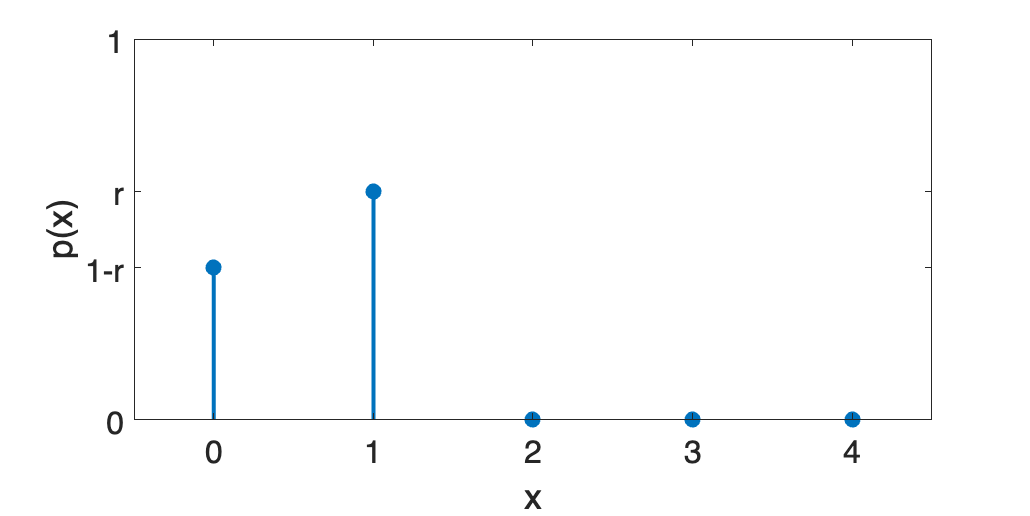
\includegraphics[width=.9\linewidth]{figures/bern.pmf.png}
  \caption{PMF.}
  \label{fig:bern:pmf}
\end{subfigure}\hfill
\begin{subfigure}{.5\textwidth}
  \centering
  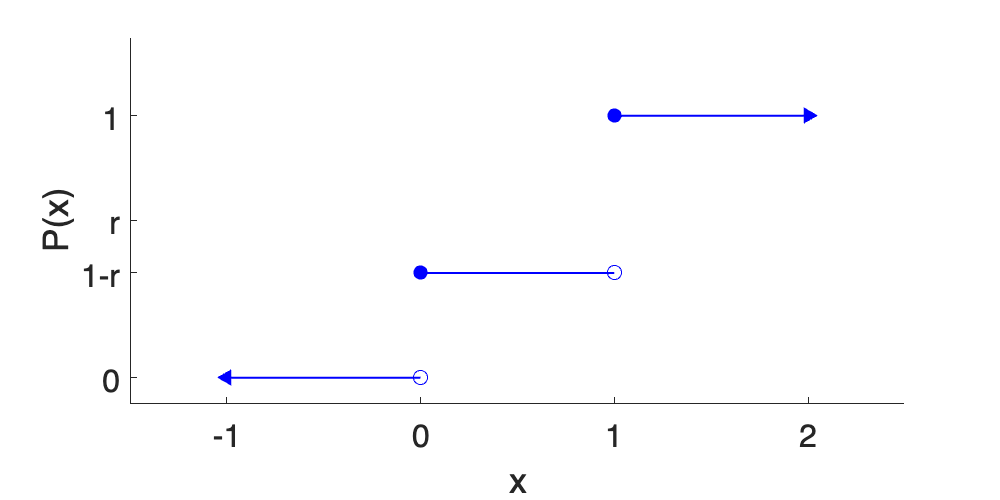
\includegraphics[width=.9\linewidth]{figures/bern.cdf.png}
  \caption{CDF.}
  \label{fig:bern:cdf}
\end{subfigure}
\caption[An example of the Bernoulli distribution.]{Bernoulli distribution.}
\label{fig:bern}
\end{figure}

The pmf and the cdf of the Bernoulli distribution can be seen on Figure \ref{fig:bern}.
We denote this distribution as $p(x) = \operatorname{Bernoulli}(x;r)$.
The expected value and the covariance of a Bernoulli random variable $X$ are

$$
E[X] = r, \qquad \operatorname{Var}[X] = r(1-r).
$$

In object tracking, we use Bernoulli random variables to model the existence of
an object at some time step $k$, which we will discuss in detail in the following
sections.

            \subsubsection{Binomial distribution}\label{sec:binomial-distribution}
                Binomial random variables are the generalization of Bernoulli random variables,
representing the probability of $x$ positive outcomes after $n$ consecutive and
independent trials. This distribution is parameterized by the probability of the
positive outcome in one trial $r$ and the number of trials $n$. Its pmf, as well 
as the expected value and the variance, are given by

\begin{equation}
\begin{aligned}
    p(x) &= \binom{n}{x} r^x (1-r)^{(n-x)}, \\
    E[X] &= nr, \\
    \operatorname{Var}[X] &= nr(1-r).
\end{aligned}
\end{equation}

            \subsubsection{Poisson distribution}\label{sec:poisson-distribution}
                The Poisson distribution is a discrete random distribution that can 
be used as an approximation of the Binomial distribution in cases where 
$n$ tends towards infinity and $r$ tends towards $0$ such that their 
product stays about equal to a parameter $\lambda$, which is the 
parameter of the Poisson distribution and also its expected value and 
variance. The outcome space of a Poisson random variable is 
$\mathbb{N}_0$, that is natural numbers including $0$, and its pmf,
expected value and variance are given by

\begin{align}
    p(x) = \operatorname{Poisson}(x; \lambda) &= \frac{\lambda^x e^{-\lambda}}{x !}, \\
    E[X] = \operatorname{Var}[X] &= \lambda.
\end{align}

The probability mass function and the corresponding cumulative density functions
of the Poisson distribution can be seen in Figure \ref{fig:poisson}.
The Poisson distribution is a critical component of modern multi-object
tracking systems, as it is used to model noise measurements, and some 
systems even use it to model objects that exist but are not visible in
the field of view of a sensor \cite{garcia-fernandezPoissonMultiBernoulliMixture2018}.
The Poisson distribution is the foundation of the so-called Poisson Point
Processes (PPP), which will be discussed later.

\begin{figure}
\centering
\begin{subfigure}{.5\textwidth}
  \centering
  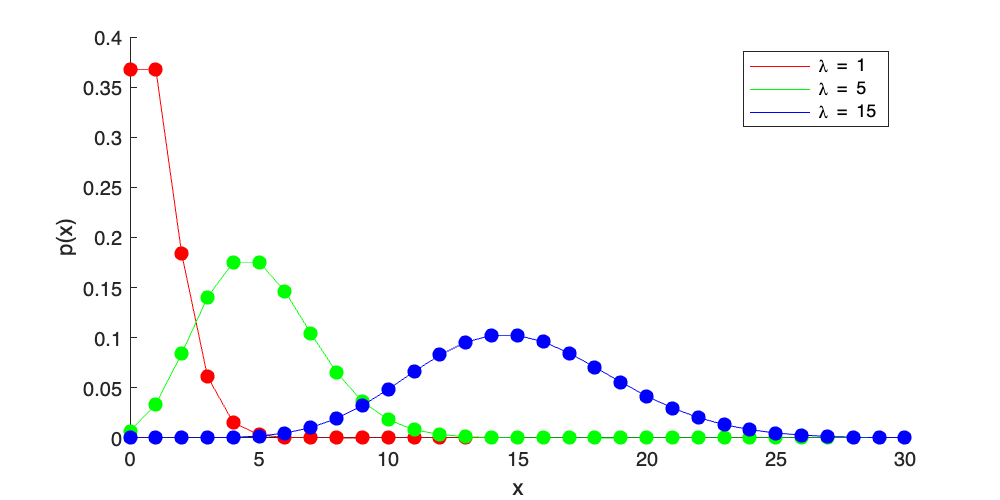
\includegraphics[width=.9\linewidth]{figures/poisson.pmf.png}
  \caption{PMF.}
  \label{fig:poisson:pmf}
\end{subfigure}\hfill
\begin{subfigure}{.5\textwidth}
  \centering
  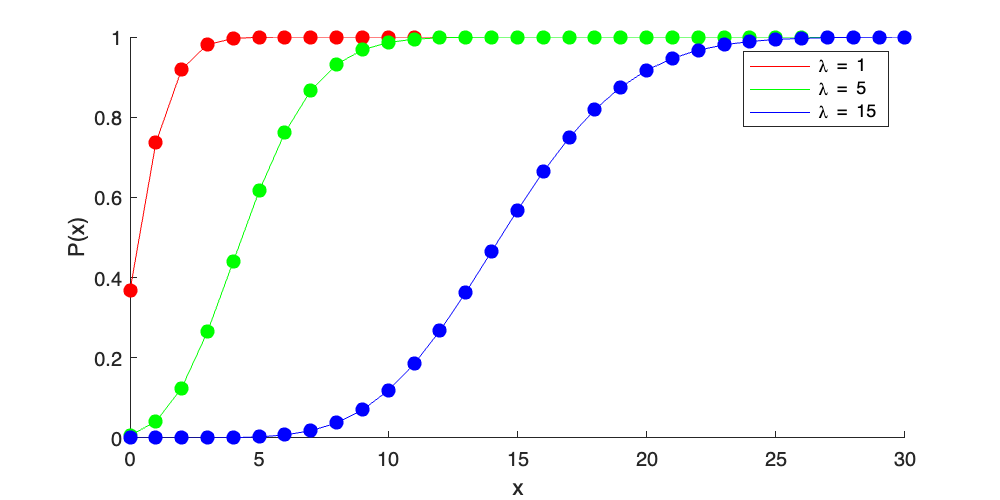
\includegraphics[width=.9\linewidth]{figures/poisson.cdf.png}
  \caption{CDF.}
  \label{fig:poisson:cdf}
\end{subfigure}
\caption[An example of the Bernoulli distribution.]{Poisson distribution.}
\label{fig:poisson}
\end{figure}

            \subsubsection{Uniform distribution}\label{sec:uniform-distribution}
                The uniform distribution is a continuous probability distribution and it
describes such random variables which outcomes on some interval $[a, b]$
are possible with equal probability. This distribution is parameterized by
$a$ and $b$ and its pdf, $E[X]$ and $\operatorname{Var}[X]$ are:

\begin{align}
    p(x)
        =\operatorname{Uniform}(x; [a, b])
        &= \begin{cases}
            \frac{1}{b-a} & \text { if } a \leq x \leq b, \\
            0 & \text { otherwise, }
        \end{cases} \\
    E[X] &= \frac{a + b}{2}, \\
    \operatorname{Var}[X] &= \frac{(b - a)^2}{12}.
\end{align}

The uniform distribution is generally used to represent the uncertainty when
all outcomes are equally possible. In this work, we use the uniform distribution
to model positions of clutter measurements at some time step $k$.

            \subsubsection{Gaussian distribution}\label{sec:gaussian-distribution}
                The Gaussian distribution, also known as the normal distribution, is a 
continuous probability distribution that is widely used in many branches
of statistics, including Bayesian filtering. It is typically used to model
a large number of independent and identically distributed (i.i.d.) random variables.

The Gaussian distribution is characterized by two parameters: the mean 
$\mu$ and the variance $\sigma^2$. Its probability density function (pdf), 
expected value, and variance are given by:

\begin{align}
    p(x)
        =\mathscr{N}\left(x ; \mu, \sigma^2\right)
        &=\frac{1}{\sqrt{2 \pi} \sigma} \exp \left(\frac{(x-\mu)^2}{2 \sigma^2}\right), \\
    E[X] &= \mu, \\
    \operatorname{Var}[X] &= \sigma^2.
\end{align}

In the notation $\mathscr{N}\left(x ; \mu, \sigma^2\right)$, the first 
parameter $x$ means ``evaluated at.''
Despite the cdf of the Gaussian distribution not having a closed-form 
representation, the distribution possesses several desirable properties that 
allow for closed-form solutions in many applications, including object 
tracking. Although it may be too simple to model certain scenarios, it 
represents the approximate average position of objects and their uncertainty 
quite well. This work utilizes mixtures of Gaussians, which will be discussed 
in more detail later.

    \section{Bayesian inference}\label{sec:bayesian-inference}
        % Bayesian inference
    % - [x] Overview of Bayesian inference and its advantages over frequentist methods
    % - [x] Sequential application
% Estimators
    % - [x] MLE and MAP
    % - [x] What is better and why

In statistics, there are two ways to understand the uncertainty. The first one,
called \textit{frequentist}, assumes that the source of uncertainty lays in the
nature of events. If we modeled a random process following this approach, we 
would calculate parameters of the model using their maximum likelihood 
estimation, which in fact is the probability density function if the parameter 
evaluated at the observed data (we will talk more about estimators in Section 
\ref{sec:estimators}). In addition to the estimated parameter 
value, we could also calculate confidence intervals, which would give us a 
range where a possible true value of the parameter can lay considering some 
probability of possible error.

The \textit{Bayesian} approach has a different philosophy. It main
assumption is that the uncertainty origin is in the modeling itself and that
this are we who have limited knowledge about the ground true model. This
difference leads to a completely distinct path of estimating values of a model.
At the beginning, we give parameters a \textit{prior distribution}, our
initial belief where true values of parameters may lay. Next, after every new
data piece we update the distribution using the Bayes' rule. Using the
\textit{likelihood function}, which represents our updated beliefs about the
parameter after observing the data, and the prior, we compute the
\textit{posterior distribution}, the updated belief about the value of the
parameter. And, in an every subsequent step, the posterior becomes a new prior.

One of the main differences, however, in these two approaches is the output of 
such estimation. While in the frequentist statistics we get values of 
parameters, the Bayesian approach will give us a full posterior distribution of 
parameter values. From such a distribution, we can extract information for our 
needs, such as an estimation of a value or some uncertainty measure.

In object tracking, the Bayesian approach to estimation has several advantages. 
Firstly, we can estimate the posterior as time passes, one measurement at a 
time. This is good because rarely do we have all measurements in advance, and 
often we want our systems to work in an online manner. Secondly, full 
posteriors allow us to work with the uncertainty of estimation and implement 
techniques to reduce the number of new hypotheses using merging 
techniques.\footnote{
    As we will see later, the GM-PHD filter uses the Mahalanobis distance 
    between Gaussians to decide what hypotheses should be merged into one. The 
    computation of Mahalanobis distance includes the covariance matrix.
}

Last but not least, the Bayesian approach allows us to incorporate prior 
knowledge about the motion models of objects and their birth positions. All of 
the above helps to improve tracking performance and reduce the impact of noisy 
measurements.

        \subsection{Bayes' rule in terms of pdfs}\label{sec:bayes-rule-pdf}
            In Bayesian object tracking, probability distributions are used instead of pure 
probabilities. Therefore, Bayes' rule must be defined using distributions. 
Fortunately, this is straightforward after we define the conditional probability in terms of pdfs.

\begin{definition}[Conditional probability for pdfs]\label{def:cond-prob-pdf}
    Let $x$ and $y$ be random variables with pdfs $p(x)$ and $p(y)$, respectively, and the joint distribution $p(x,y)$. Then the conditional probability of $x$ given $y$ is defined as:
    \begin{equation*}
        p(x|y) = \frac{p(x,y)}{p(y)}.
    \end{equation*}
\end{definition}

\begin{definition}[Bayes' rule for pdfs]
    Let $z$ and $x$ be random variables with densities $p(z | x)$ and $p(x)$, 
    respectively, and let $p(z, x)$ be their joint distribution. The Bayes' rule
    for 
    $p(x | z)$ is defined as follows:

    $$
    p(x | z)
        = \frac{p(z | x) p(x)}{p(z)}
        = \frac{p(z | x) p(x)}{\int p(z | x) p(x) dx}.
    $$
\end{definition}

The distribution $p(x | z)$ is the posterior distribution, $p(z | x)$ is the 
likelihood, $p(x)$ is the prior, and $p(z)$ is called \textit{evidence}.

Evidence here is only the normalization constant for the distribution so
that the integral of the posterior equals to one. It is therefore convenient
to omit this denominator in the text and write the posterior only in terms of
prior and likelihood. Since it is not already the equality, we use the
proportionality symbol:

$$
p(x | z) \propto p(z | x) p(x).
$$

We can use the rule defined above to compute the posterior of some parameter
based on all the data. However, in many real-world applications, measurements
do not arrive all at once, but rather sequentially over time. In the context of 
object tracking, sensors generate measurements in a discrete manner, once per
some predefined time interval, and the goal of the tracking algorithm to 
estimate targets' state at each time step. Fortunately, the construction of the
Bayes' rule allows us to define the sequential data update in a very 
straightforward manner.

\begin{theorem}[Sequential Bayes' rule]
    Let $z_k$ be an observed random variable at discrete time steps
    $k = 1, 2, \ldots$ and let $z_{1:k-1}$ represent the realizations of $z_k$ 
    obtained from the time step $k = 1$ up to $(k-1)$, that is $z_{1:k-1} = 
    \{z_1, z_2,\ldots, z_{k-1}\}$. Let $p(x_k | z_{1:k-1})$ denote the posterior 
    distribution obtained at time $k-1$ using all the measurements up to $k-1$ 
    and $p(z_k | x_k)$ be the likelihood of the new measurement $z_k$. The 
    posterior distribution $p(x_k | z_{1:k})$ at time step $k$ is:
    \todo{The alignment of the formula is awful. Check later}
    $$
    p(x_k | z_{1:k}) 
        = \frac
            { p(z_k | x_k) p(x_k | z_{1:k-1}) }
            { p(z_k | x_k) p(x_k | z_{1:k-1}) dx_k }
        \propto p(z_k | x_k) p(x_k | z_{1:k-1}).
    $$
\end{theorem}

It should be mentioned that $x_k$ and $z_k$ must not always be scalars. As we
will later see, they can be vectors, denoted as $\mathbf{x}_k$ and 
$\mathbf{z}_k$, or even sets, denoted $X_k$ and $Z_k$. The Bayes' rule will
have the same form in any case.

The application of the Bayes' rule has one big disadvantage. In practice, 
calculating the posterior can be challenging or even intractable. The evidence 
term in the denominator contains the integral of the product of the likelihood 
and the prior over the whole measurement space. This product may (and often 
will) produce functions whose integration cannot be expressed in a closed-form 
solution.

However, we can obtain a tractable solution by choosing a prior distribution 
from a set of \textit{conjugate distributions} with respect to the likelihood. 
In this case, the posterior will be in the same form as the prior and we obtain 
an explicit closed-form solution. A conjugate prior for a given likelihood 
function is a prior distribution that, when used in combination with the 
likelihood, leads to a posterior distribution that is in the same family as the 
prior.

For example, if the likelihood is expressed using the Bernoulli distribution 
and the prior is the Beta distribution, the posterior will also be a Beta 
distribution. The same applies for the Gaussian distribution, where if both the 
prior and the likelihood are Gaussian, the posterior is also Gaussian. This is 
particularly useful in practice, as many distributions have well-known 
conjugate priors. The latter case is used, for instance, in the GM-PHD filter.

        \subsection{Estimators}\label{sec:estimators}
            As mentioned before, the output of the Bayesian inference is always a
distribution. However, we are often interested in obtaining an estimated value
of the parameter we are estimating. \textit{Estimators} do exactly that.
Strictly speaking, estimators take a set of observations and produce an 
estimate of the value of an unknown parameter of a distribution. We denote an
estimate of an unknown parameter $x$ as $\hat{x}$. There are several known 
estimators but we are interested in two of them: ML and MAP.

The \textit{Maximum Likelihood (ML)} estimator finds the value of the parameter 
such that it maximizes the likelihood function. Formally:

$$
\hat{x}_{\mathrm{ML}} = \arg \max_x p(z|x).
$$

The ML estimator is a point estimator that finds the parameter value that 
makes the observed data most probable. For instance, the frequentist approach
uses this estimator to find the parameter value. The MLE does not take the 
prior distribution into account and is more sensitive to outliers. 
\todo{Citation needed}

The \textit{Maximum A Posteriori (MAP)} estimator, on the other hand, finds the 
value of the parameter that maximizes the posterior distribution. In formal 
notation:

$$
\hat{x}_{\mathrm{MAP}} = \arg \max_x p(x|z) = \arg \max_x p(z|x)p(x).
$$

The MAP estimator finds the most probable value of the parameter given the 
observed data. Comparing to the MLE, MAP uses prior information and more robust
when the data is noisy or incomplete. That is the reason why MAP is often used
in Bayesian inference.\footnote{
    In this work, we use Gaussian posterior distributions and MAP estimates are 
    equal to posterior mean estimates, or MMSE-estimates. However, for general 
    distributions, it will rarely be the case.
}

    \section{Gaussian-linear Bayesian filtering}\label{sec:gauss-linear-filtering}
        We have now introduced the main principles of Bayesian inference. Now, we can
turn to the Kalman filter, a popular and widely used algorithm for state 
estimation. The Kalman filter (KF, for short) is a recursive algorithm that uses
Bayesian inference to estimate the state of a dynamic system based on a sequence
of noisy measurements.

The key feature of the KF is the ability to predict future states of the system.
This is essential for applications that require to foresee the behavior of
tracked objects before the state of these objects is measured. Examples of such
systems may include autonomous driving or air defence systems. The prediction 
ability helps also to overcome situations when a sensor fails to measure the
position of an object (a so-called misdetection).

In the following subsections, we will introduce the state-space models, give
a formal definition of a general Bayes filter, infer the Kalman filter formulas
and discuss the Constant Velocity (CV) model, a common motion model used in the
Kalman filter.

        \subsection{Multivariate Gaussian Distribution}\label{sec:multivariate-gaussian}
            Before we start learning the basics of Bayesian filtration, we should extend our knowledge of the Gaussian distribution to the multidimensional case. As mentioned in Section \ref{sec:gaussian-distribution}, it plays a very important role in object tracking and, in particular, in this work. Formulas and theorems defined in this section are essential for defining and proving the Kalman filter formulas. We will define several properties of multivariate Gaussians required later.

First, we define the multivariate Gaussian distribution with mean vector $\boldsymbol\mu$, covariance matrix $\Sigma$, and evaluated at $\mathbf{x}$ as:

\begin{equation}\label{eq:vec-gauss-def}
    \mathscr{N}\left(\mathbf{x} ; \mathbf\mu, \mathbf\Sigma\right)
    = \frac{1}{\sqrt{(2\pi)^n|\mathbf{\Sigma}|}}\exp\left(-\frac{1}{2}(\mathbf{x}-\boldsymbol{\mu})^\top \mathbf{\Sigma}^{-1} (\mathbf{x}-\boldsymbol{\mu})\right),
\end{equation}

\noindent where $n$ is the length of the vector $\mathbf{x}$, and $|\cdot|$ denotes the determinant of a matrix. 

The multivariate Gaussian distribution is a generalization of the univariate Gaussian distribution, where instead of a single mean and variance, we have a mean vector and a covariance matrix that characterizes the correlation between the variables. Note that the exponent contains the expression known as the Mahalanobis distance, which we will encounter throughout this work. It is given by:

\begin{definition}[Mahalanobis distance]\label{def:mahalanobis}
    For vectors $\mathbf x$ and $\mathbf y$ and the symmetrical positive-definite matrix $\mathbf S$, the Mahalanobis distance is defined as:

    \begin{equation}
        d(\mathbf x, \mathbf y) 
        = \sqrt{
            (\mathbf x - \mathbf y)^\intercal
            \mathbf{S}^{-1}
            (\mathbf x - \mathbf y)
        }.
    \end{equation}
\end{definition}

As we will later see, in object tracking, we heavily use conditional probabilities, and in particular, conditioning and marginalization of joint distributions of Gaussian random variables. Thus, we define the following two theorems.

\begin{theorem}[Conditioning on a Gaussian joint distribution]\label{theorem:gauss-cond}
    Let $\mathbf{x}$ and $\mathbf{y}$ be Gaussian random variables with distributions $\mathscr{N}\left(\mathbf{x} ; \mathbf\mu_x, \mathbf\Sigma_{xx}\right)$ and $\mathscr{N}\left(\mathbf{y} ; \mathbf\mu_y, \mathbf\Sigma_{yy}\right)$, respectively. Let their joint probability be given by:

    \begin{equation}
        p(\mathbf{x}, \mathbf{y}) = \mathscr{N}\left(
            \begin{bmatrix}
                \mathbf{x} \\
                \mathbf{y}
            \end{bmatrix};
            \begin{bmatrix}
                \boldsymbol\mu_x \\
                \boldsymbol\mu_y
            \end{bmatrix},
            \begin{bmatrix}
                \mathbf{\Sigma}_{xx} & \mathbf{\Sigma}_{xy} \\
                \mathbf{\Sigma}_{xy}^\intercal & \mathbf{\Sigma}_{yy}
            \end{bmatrix}
        \right).
    \end{equation}
    \noindent Then the conditional distribution of $\mathbf{x}$ given $\mathbf{y}$ is defined as:
    \begin{equation}\label{eq:gauss-cond}
        p(\mathbf{x}|\mathbf{y}) =
        \mathscr{N}\left(\mathbf{x}; \boldsymbol\mu_{x|y}, \mathbf\Sigma_{x|y}\right),
    \end{equation}
    \noindent where
    \begin{align}
        \boldsymbol\mu_{x|y}
        &= \boldsymbol\mu_x + \mathbf{\Sigma}_{xy} \mathbf{\Sigma}_{yy}^{-1}(\mathbf{y} - \boldsymbol\mu_y), \\
        \mathbf\Sigma_{x|y} 
        &= \mathbf\Sigma_{xx} - \mathbf\Sigma_{xy}\mathbf\Sigma_{yy}^{-1}\mathbf\Sigma_{xy}^\intercal.\label{eq:gauss-cond-params}
    \end{align}
\end{theorem}

\begin{theorem}[Marginalization of a Gaussian joint distribution]\label{theorem:gauss-marg}
    Consider the same $\mathbf{x}$, $\mathbf{y}$, $\mathscr{N}\left(\mathbf{x} ; \mathbf\mu_x, \mathbf\Sigma_{xx}\right)$, $\mathscr{N}\left(\mathbf{y} ; \mathbf\mu_y, \mathbf\Sigma_{xx}\right)$ and $p(\mathbf{x}, \mathbf{y})$ given in Theorem \ref{theorem:gauss-cond}. The marginal distribution of $x$ is defined as:

    \begin{equation}
        p(\mathbf{x}) = \mathscr{N}\left(\mathbf{x} ; \mathbf\mu_x, \mathbf\Sigma_{xx}\right).
    \end{equation}
\end{theorem}

The proofs for Theorem \ref{theorem:gauss-cond} and Theorem \ref{theorem:gauss-marg} can be found in classical statistical textbooks such as \cite[161--163]{johnsonAppliedMultivariateStatistical2007}.

            \subsubsection{Gaussian mixtures}\label{sec:gaussian-mixtures}
                In multi-target tracking, the posterior density cannot be described in a simple Gaussian distribution. Generally, the posterior distribution can have any form with only assumption that the integral of it sums to one. However, when we are dealing with Gaussian-linear cases, the posterior density is often represented as a mixture of many Gaussian components. A Gaussian mixture is a linear combination of multiple Gaussian distributions and its pdf is expressed in the following way:

\begin{equation}\label{eq:gaussian-mixture}
    p(\mathbf{x}) = \sum_{i=1}^N w_i \mathscr{N}\left(\mathbf{x}; \boldsymbol{\mu}_i, \Sigma_i\right),
\end{equation}

\noindent where $N$ is the number of Gaussian components in the mixture, $w_i$ is the weight of the $i$th component, the weights $w_i \geq 0$ sum to one, i.e. $\sum_{i=1}^N w_i = 1$, and each component $\mathscr{N}\left(\mathbf{x}; \boldsymbol{\mu}_i, \Sigma_i\right)$ is a Gaussian distribution with the mean in $\boldsymbol{\mu}_i$ and the covariance matrix $\Sigma_i$. An example of a Gaussian mixture pdf is illustrated in Figure \ref{fig:gaussian-mixture}.

\begin{figure}
\centering
  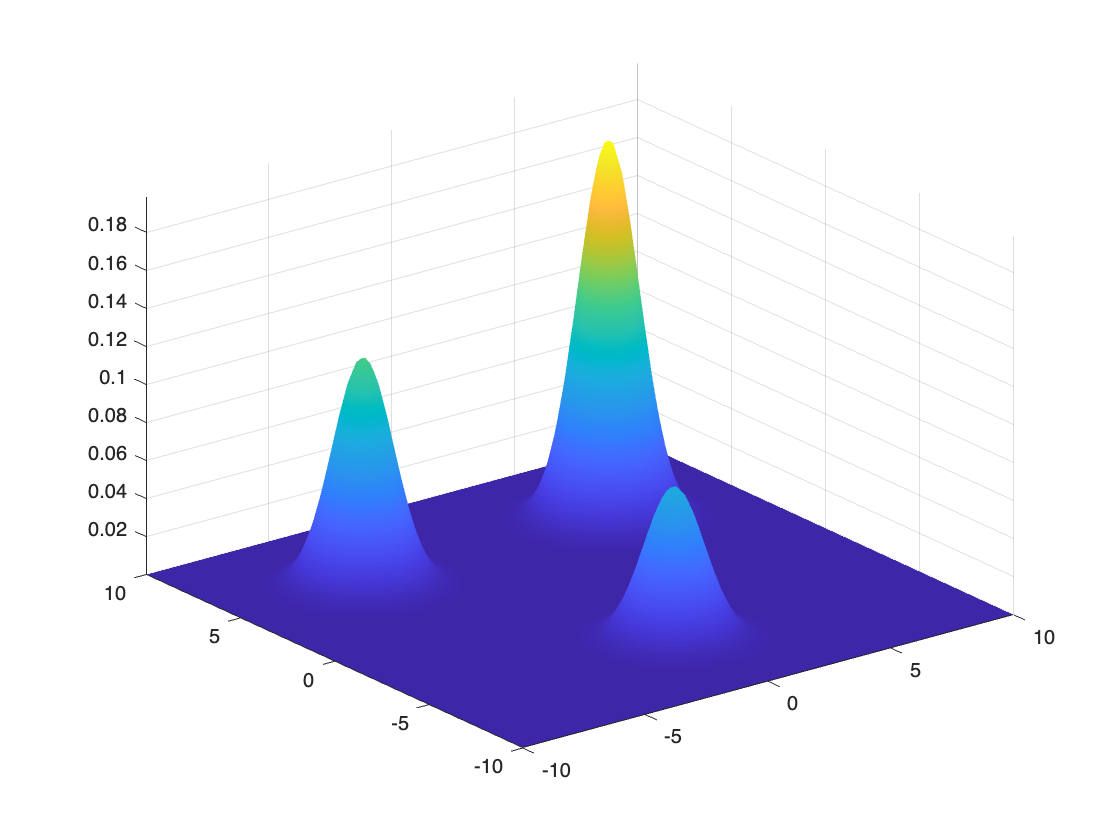
\includegraphics[width=.6\linewidth]{figures/gaussian-mixture.png}
  \caption{An example of a Gaussian mixture with three components. The first component is centered at $[0, -5]^\intercal$ with weight $0.2$, the second component has mean in $[-5, 5]^\intercal$ with weight $0.3$ and the last has mean $[5, 5]^\intercal$ and the weight $0.5$.}
  \label{fig:gaussian-mixture}
\end{figure}

Since the weights sum to one, the Gaussian mixture satisfies the normalization requirement of pdfs and is thus a valid probability density function itself. The weights in the mixture represent the relative importance of the corresponding component. Gaussian mixtures are used to model complex distributions and have several nice mathematical properties as the Gaussian distribution, as we will later see. That is why Gaussian mixtures are widely used to represent posterior distributions in many MTT filters. Moreover, one can easily approximate any distribution with a Gaussian mixture using algorithms such as the Expectation-Maximization algorithm.

A mixture $f(\mathbf{X})$ with $N$ components will have the expected value $\boldsymbol{\hat{\mu}}$ and the covariance $\hat{\Sigma}$ according to the following equations:

\begin{align}
    \boldsymbol{\hat{\mu}} &= \sum_{i=1}^N w_i \boldsymbol{\mu}_i, \\
    \hat{\Sigma} &= \sum_{i=1}^N w_i \Sigma_i + \Tilde{\Sigma},
\end{align}

\noindent where the term $\Tilde{\Sigma}$ is called the spread-of-the-innovations and is defined as:

\begin{equation}
    \Tilde{\Sigma}= \sum_{i=1}^N
        w_i (\boldsymbol{\mu}_i - \hat{\boldsymbol{\mu}})
        (\boldsymbol{\mu}_i - \hat{\boldsymbol{\mu}})^\intercal.
\end{equation}

The spread-of-the-innovations quantifies the magnitude of the difference between expectations of individual components.

        \subsection{State-space model}\label{sec:state-space}
            In the previous section, we established the relationships between prior and 
posterior distributions and learned about recursive Bayesian estimation of the 
posterior. Now, we will explore these concepts in the context of object 
tracking.

Object tracking involves estimating the internal states of objects that move in 
some space, which are often unknown to us. These states may include physical 
properties of objects such as position, velocity, acceleration, and 
orientation, depending on the application. Sensors such as cameras, infrared 
scanners, lidars or radars constantly generate measurements of the object 
states, which may be the distance of an object to the sensor, or its 
temperature. However, these measurements are often noisy due to environmental 
conditions or imperfections of the sensor. We use Bayesian filtering to 
estimate the real state of the objects and filter out the noise.

To handle the complexity and diversity of possible situations and properties, 
we need a systematic framework for modeling object motion that captures all 
sources of uncertainty and the nature of physical behavior of objects. This 
framework is called state-space modeling. In state-space models, the internal 
state we want to estimate is represented as a vector of variables that evolve 
over time according to a set of rules specified by the \textit{motion model}, 
which is a known function. The measurements obtained at each time step are 
modeled as a different function of the state variables, known as the 
\textit{measurement model}\footnote{
    It should be mentioned that the names `motion' and `measurement' models are 
    not the only terms used to describe them. The reader may also encounter 
    terms such as kinematic, state-transition, dynamic, or system models for the 
    motion model, and terms like observation, sensor, or likelihood models for 
    the measurement model. All of these names are correct, and their use depends 
    on the context in which they are applied. However, in this work, the author 
    strives for consistency and will use the terms `motion' and `measurement' 
    models throughout the entire text.
}.

For example, consider a moving bicycle and a surveillance camera with a 
rectangular field of view (FoV). The bicycle enters the FoV and crosses it at a 
constant speed. The camera has an algorithm that estimates the position of 
objects in the space from the image. With each frame $f$, it returns a new 
position, say $(\hat x_f, \hat y_f)$. We can represent the state of the bicycle 
as a vector of the position and velocity, which are unknown variables. Based on 
the measurements, we estimate their values using the known physical relation 
between distance, velocity, and time: $d = v \Delta t$, where $d$ is the 
distance that the object with velocity $v$ traveled in time $\Delta t$.

Both the motion and measurement models should include some noise. In the 
example above, the movement of the bicycle cannot perfectly follow the formula, 
and there will always be some minor changes in speed. Moreover, the measurement 
model, which translates an estimated state into a measurement, will also 
contain some uncertainty since the camera does not have a perfect 
representation of the space.

We can now describe these models formally. Note that since the state is a 
vector, we will use $\mathbf{x}$ for vectors. The motion and measurement models 
can be generally expressed as:

\begin{align}
    p(\vecat{x}{k} | \vecat{x}{k-1}) 
        &= f_t(\vecat{x}{k-1}, \vecat{u}{k}, \vecat{w}{k}), \\
    p(\vecat{z}{k} | \vecat{x}{k}) 
        &= h_t(\vecat{x}{k}, \vecat{v}{k}),
\end{align}

\noindent where $f_t$ and $h_t$ are functions, $\vecat{x}{k-1}$ is the estimated state 
from time step $k-1$, $\vecat{u}{k}$ is called the input (or control) vector, 
and $\vecat{w}{k}$ and $\vecat{v}{k}$ are zero-mean noise random variables.

However, this definition is too general since the functions $f_t$ and $h_t$ can 
be anything. As mentioned earlier, to get a closed-form solution in the 
Bayesian inference framework, we need to choose conjugate distributions for the 
likelihood and the prior. The Kalman filter, which we will describe soon, works 
for the Gaussian-linear case, where the functions $f_t$ and $h_t$ are linear 
and noise variables are distributed as Gaussian, i.e., 
$\vecat{w}{k}, \vecat{v}{k} \sim \mathscr{N}(\mathbf{0}, \Sigma)$. The Gaussian-
linear state-space model has the following representation:

\begin{align}
    p(\vecat{x}{k} | \vecat{x}{k-1}) 
        &= \mathbf{F} \vecat{x}{k-1}
            + \mathbf{B} \vecat{u}{k}
            + \vecat{w}{k},
        & \vecat{v}{k} \sim \mathscr{N}(\mathbf{0}, \mathbf{Q}), \\
    p(\vecat{z}{k} | \vecat{x}{k})
        &= \mathbf{H} \vecat{x}{k} + \vecat{v}{k},
        & \vecat{w}{k} \sim \mathscr{N}(\mathbf{0}, \mathbf{R}), \\
    p(\vecat{x}{0}) &\sim \mathscr{N}(\vecat{\hat{x}}{0}), \vecat{P}{0}),&
\end{align}

\noindent where:

\begin{itemize}
    \item $\mathbf{F}$ is the \textit{transition matrix},
    \item $\mathbf{B}$ is the \textit{input matrix},
    \item $\mathbf{H}$ is the \textit{measurement matrix},
    \item $\mathbf{Q}$ and $\mathbf{R}$ are symmetric positive definite matrices
        that describe the statistical properties of the motion noise
        \vecat{v}{k} and the measurement noise \vecat{w}{k}, respectively,
    \item $\vecat{\hat x}{0}$ and $\vecat{P}{0}$ are mean and variance of the 
    prior state.
\end{itemize}

The control variable $\vecat{u}{k}$, in general, represents some input signal from the environment, and $\mathbf{B}$ specifies how the input signal affects the dynamic system. This may include the effect of gravity on the vertical traveled distance or the voltage applied to some circuit. However, in object tracking, we rely on measurements obtained from sensors to update our estimate of the object's state. We do not have control over the object's motion. Thus, the input matrix is often redundant, and we omit it (or set it to a zero matrix) along with the input variable $\vecat{u}{k}$.

The notation above may be inconvenient in some cases. In this work, we will often use a shorter version that has the same meaning:

\begin{align}
    p(\vecat{x}{k} | \vecat{x}{k-1})
        &= \mathscr{N}(\vecat{x}{k}; \mathbf{F}\vecat{x}{k-1}, \mathbf{Q}), 
        \label{eq:motion-model} \\
    p(\vecat{z}{k} | \vecat{x}{k})
        &= \mathscr{N}(\vecat{z}{k}; \mathbf{H}\vecat{x}{k}, \mathbf{R}), 
        \label{eq:measurement-model} \\
    \vecat{x}{0}
        &\sim \mathscr{N}(\vecat{x}{0}; \vecat{\hat{x}}{0}, \vecat{P}{0}).
        \label{eq:prior-x0}
\end{align}

            \subsubsection{Constant Velocity Model}\label{sec:cv-model}
                The Constant Velocity (CV) model is one of the most commonly used motion and measurement models in the context of object tracking. It describes the kinematics of objects in a 2D space that move with a constant velocity. The state vector comprises a position vector and a velocity vector, and while the position vector contains the coordinates of the object in the space, the velocity vector contains the object speed in the direction of each axis.

The CV model is linear and one of the simplest models. It assumes that the speed of objects remains unchanged during tracking, with only small deviations from the constant. This model can be reasonably utilized in scenarios where objects do not change their speed or direction, such as vehicles on highways or planes in the sky. Since the state vector contains only four variables, the use of this model does not increase the computational burden on tracking algorithms.

The motion equation for the CV model is given by \ref{eq:motion-model}, and the state vector $\vecat{x}{k}$, the state transition matrix $\mathbf{F}$, and the process noise matrix $\mathbf{Q}$ can be defined as:

\begin{equation}
    \vecat{x}{k} =
    \begin{bmatrix}
        x_{1,k} \\ 
        x_{2,k} \\ 
        v_{x_1,k} \\ 
        v_{x_2,k}
    \end{bmatrix};
    \quad
    \mathbf{F} =
    \begin{bmatrix}
       1 & 0 & dt & 0 \\
       0 & 1 & 0 & dt \\
       0 & 0 & 1 &  0 \\
       0 & 0 & 0 &  1 
    \end{bmatrix};
    \quad
    \mathbf{Q} = q^2 \cdot
    \begin{bmatrix}
        \frac{dt^3}{3}    & 0                 & \frac{dt^{2}}{2}  & 0  \\
        0                 & \frac{dt^3}{3}    & 0                 & \frac{dt^{2}}{2} \\
        \frac{dt^{2}}{2}  & 0                 & dt                & 0 \\
        0                 & \frac{dt^{2}}{2}  & 0                 & dt
    \end{bmatrix},
\end{equation}

\noindent where $dt$ is the change in time between the last estimation and the newly computed one, and $q$ is the motion noise parameter, which represents the uncertainty in the state transition.

The measurement model transforms a state vector from the state space into the measurement space. Since the vanilla Kalman filter, which we will derive soon, works only with linear models, the measurement model for the CV model assumes sensors measurements in the same 2D space as in the state vectors. The measurement equation is given by \ref{eq:measurement-model}, and the measurement matrix $\mathbf{H}$ and the measurement noise matrix $\mathbf{R}$ can be defined as:

\begin{equation}
    H =
    \begin{bmatrix}
        1 & 0 &0 & 0 \\
        0 & 1 &0 & 0
    \end{bmatrix};
    \quad
    R =
    r^{2}\cdot
    \begin{bmatrix}
        1 & 0 \\
        0 & 1
    \end{bmatrix},
\end{equation}

\noindent where $r$ is the measurement noise parameter, which determines the variance of the measurement noise.

We need to describe the choice of parameters $q$ and $r$ in more detail. These parameters are crucial in obtaining good estimates from a filter. These parameters are not known a priori and their values should be chosen carefully by the means of trial and error, or using automated methods like, for instance, in \cite{bulutProcessMeasurementNoise2011}. However, selecting appropriate values often involves a trade-off between tracking accuracy and computational complexity, and the use of exact methods depends on the application and one's requirements.

The CV model can be extended with additional information, such as change of speed. In this way we will come to the constant acceleration model. However, it will not be used in this work and, therefore, we will not leave formal definition of this model here.

        \subsection{The Bayes filter}\label{sec:bayes-filter}
            We have learned how the internal state of a system can be represented in terms
of a state vector and motion and measurement models. Now, we are ready to 
present the formal definition of the Bayes filter, the general abstraction of
any Bayesian filter, including the Kalman filter and the PHD filter.

First, we need to make a very important assumption on states. This assumption
is called the \textit{Markov model property}. This property states that, for 
the motion model, the present state of a system $x_k$ is dependent only on 
the state on the previous time step $x_{k-1}$ given all past states $x_{1:k-1}$ 
and measurements $z_{1:k-1}$. More formally:

\begin{equation}
p(x_k | x_1, \ldots, x_{k-2}, x_{k-1},
        z_1, \ldots, z_{k-2}, z_{k-1}) 
    = p(x_k | x_{k-1}).
\end{equation}

A similar requirement must hold for measurement model, that is:

\begin{equation}
    p(z_k | x_1, \ldots, x_{k-2}, x_{k-1}, x_{k}
        z_1, \ldots, z_{k-2}, z_{k-1}) 
    = p(z_k | x_k).
\end{equation}

The Markov property may seem restrictive but in reality it is not because state-
space models allows us to capture dependencies in the system dynamics by simply 
introducing more variables into the state vector. For instance, if we have a 
system where the current state has a dependence on the previous two states, we 
can augment the state vector to include the last two states as variables, and 
the Markov property will still hold.

The Bayes filter uses the motion and measurement models and assumes that this
property holds. The Bayes filter is a recursive framework that estimates an
internal state of the system over time using measurements. Every iteration of
the filter consists of two steps: prediction and update. On the prediction step,
the filter estimates a internal state $x_k$ based on the previous state
$x_{k-1}$ and the motion model $p(x_k | x_{k-1})$. The prediction step
is also known as the Chapman-Kolmogorov equation.

\begin{theorem}[The prediction step. The Chapman-Kolmogorov equation]\label{theorem:bayes-filter-predict}\label{theorem:chapman-kolmogorov}
    Given the set of measurements $z_{1:k-1} = \{z_1, z_2, \ldots, z_{k-1}\}$ 
    and the current state $x_{k-1}$ and the motion model $p(x_k | x_{k-1})$, 
    the prediction step of the Bayes filter is computed as follows:

    \begin{equation}
        p\left({x}_k | {z}_{1: k-1}\right)
        = \int 
            p\left(
                {x}_k, {x}_{k-1} | {z}_{1: k-1}
            \right)
            \mathrm{d} {x}_{k-1}
        = \int
            p\left(
                {x}_k | {x}_{k-1}\right
            ) p\left(
                {x}_{k-1} | {z}_{1: k-1}
            \right)
            \mathrm{d} {x}_{k-1}.
    \end{equation}
\end{theorem}

Next, on the update step, the filter corrects the predicted state with the 
measurement $z_k$ using the measurement model $p(z_k | x_k)$. This step is
computed using the standard Bayes' rule.

\begin{theorem}[The update step]\label{theorem:bayes-filter-update}
    Given the output of the prediction step of the Bayes filter 
    $p\left({x}_k | {z}_{1: k-1}\right)$, the observed measurement $z_k$
    and the measurement model $p(z_k | x_k)$, the update step of the Bayes
    filter is computed as follows:
    
    \begin{equation}
        p\left({x}_k | {z}_{1: k}\right)=\frac{p\left({z}_k | {x}_k\right) p\left({x}_k | {z}_{1: k-1}\right)}{p\left({z}_k | {z}_{1: k-1}\right)} \propto p\left({z}_k | {x}_k\right) p\left({x}_k | {z}_{1: k-1}\right).
    \end{equation}
\end{theorem}

These two steps create a loop, and to use the filter, we first predict the next state using the Chapman-Kolmogorov equation, and then we update our guess with a measurement. Note, that we will often use the simplified notation to explicitly state the time step of the value. The notation $\vecat{\bullet}{k|k-1}$ represents the predicted value at time step $k$, and the notation $\vecat{\bullet}{k|k}$ represents the updated value at time step $k$ after incorporating a measurement.

Now, having introduced the general Bayes filter, we will continue with 
exploring the Kalman filter in detail, the popular and widely used tool for 
state estimation.

        \subsection{The Kalman filter}\label{sec:kf-index}
            The Kalman filter is one of the most well-known and widely used algorithms in 
signal processing and control theory. It is a recursive algorithm that allows 
the estimation of internal states of entities in dynamic systems from a set of 
measurements that may be noisy or missing at some time steps. The filter was 
proposed by Rudolf Kalman in 1960 \cite{kalmanNewApproachLinear1960} and has 
since been pervasively used to control a vast array of consumer, health, 
commercial, and defense products \cite{grewalApplicationsKalmanFiltering2010}.

The development of the filter was motivated by the need to improve aerospace 
technology in the United States during the Cold War between the Soviet Block 
and the North American Treaty Organization. Because the Soviet Union managed to 
launch its artificial satellites and successfully send a human to space, the 
federal government of the United States supported research into new 
technologies in the aerospace area.

The Kalman filter is an example of a general Bayes filter that was introduced 
earlier. This means that the filter estimates the posterior distribution of the 
internal state at discrete time steps using prior information about the 
observed object's state and a set of noisy measurements. As briefly mentioned 
in Section \ref{sec:state-space}, the Kalman filter works on state-space linear 
models with Gaussian noise and a Gaussian prior of the state. The predict-
update loop in the Kalman filter is the same as in the Bayes filter, and the 
same Chapman-Kolmogorov equation defined in \ref{theorem:chapman-kolmogorov} 
and the update equation defined in \ref{theorem:bayes-filter-update} are 
incorporated.

The main advantage of the Kalman filter is that it allows for the estimation of 
the state of a system in real-time. It handles noisy measurements well and is 
fast; however, it is sensitive to initial parameter settings, such as the noise 
covariance matrices \cite{gePerformanceAnalysisKalman2016}. Nonetheless, there 
are new methods being developed that propose mechanisms to overcome this 
drawback, as in \cite{matiskoNoiseCovariancesEstimation2010} and 
\cite{yuenOnlineEstimationNoise2013}.

One of the main drawbacks of the Kalman filter is its Gaussian-linear 
assumption. In real-world applications, many systems exhibit non-linearity, and 
the Kalman filter may be ineffective. Nonetheless, several extensions of the 
filter have been proposed that address this. Two well-known algorithms are the 
Unscented Kalman Filter (UKF) and the Extended Kalman filter (EKF). The UKF is 
an algorithm that uses a set of carefully chosen sigma points to capture the 
true mean and covariance of the predicted and updated distributions without 
the need for linearization \cite{wanUnscentedKalmanFilter2000}. The EKF, on 
the other hand, linearizes the nonlinear motion and measurement models using a 
first-order Taylor expansion \cite{smithApplicationStatisticalFilter1962}. 
These methods have been proven to be effective in many applications, including 
the PHD filter. However, they are beyond the scope of this thesis and will not 
be covered in detail.

            \subsubsection{The Gaussian identity}\label{sec:gaussian-identity}
                Before we introduce the actual formulas of the Kalman filter, we should introduce a new fundamental theorem in object tracking and then deduce a corollary from it. These will also be used later when we infer formulas for the the GM-PHD filter. We define this theorem using a general notation without any meaning for Bayesian filters to avoid the confusion of variables when we use this theorem in different parts of different filters.

\begin{theorem}[The Gaussian product identity]\label{theorem:gaussian-identity}
    Given matrices and vectors $A, U, m, d$, and $V$ of appropriate dimensions, and that $U$ and $V$ are positive definite, the following identity applies:

    \begin{equation}\label{eq:gid}
        \mathscr{N}(x ; A y + d, U) \mathscr{N}(y ; m, V)=\mathscr{N}(x ; A m + d, U + A V A^\intercal) \mathscr{N}(y ; \hat{m}, \hat{V}),
    \end{equation}

    \noindent where
    \begin{align}
        \hat{m} & = m + K (y - Am - d), \\ 
        \hat{V} & = (I - K A) V, \\
        K &= V A^\intercal (U + A V A^\intercal)^{-1}.
    \end{align}
\end{theorem}

\begin{proof}\label{proof:gaussian-identity}
    The proof of Theorem \ref{theorem:gaussian-identity} presented here follows similar proofs in \cite{mahlerStatisticalMultisourcemultitargetInformation2007} (Appendix D) and \cite{risticKalmanFilterParticle2004} (Section 3.8). However, the main idea of using algebraic manipulation of matrices was taken from \cite{tokleMultiTargetTracking2018}.
    
    The proof is based on the idea that both sides of \ref{eq:gid} represent the joint Gaussian distribution of two random variables, $p(x,y)$. From \ref{def:cond-prob-pdf}, we know that we can express this distribution as:
    
    \begin{equation}
        p(x, y) = p(x|y)p(y) = p(y|x)p(x).
    \end{equation}
    
    We claim that the left-hand side (LHS) of \ref{eq:gid} represents this equality, i.e.,
    
    \begin{equation}
        p(x, y) = p(x|y)p(y) = \mathscr{N}(x ; A y + d, U) \mathscr{N}(y ; m, V).
    \end{equation}

    Next, we can express the product of two Gaussians in their quadratic forms, the same form as defined in \ref{eq:vec-gauss-def}, i.e.

    \begin{align}
        \mathscr{N}(x ; A y + d, U) \mathscr{N}(y ; m, V)
        &= \frac{1}{(2\pi)^{n} \sqrt{|U| |V|}}
        \exp \left(
        -\frac{1}{2}
        \bigg[(x - Ay - d)^\intercal U^{-1} (x - Ay - d) \right. \nonumber \\
        &\left.\qquad\qquad\qquad\qquad\qquad+ (y - m)^\intercal V^{-1} (y - m) \bigg] \right).
        \label{eq:gid-proof:lhs-expanded}
    \end{align}

    If we introduce a small algebraic trick for matrices:

    \begin{equation}
        \begin{bmatrix}
            I & -A \\
            0 & I
        \end{bmatrix}
        \begin{bmatrix}
            x - Am - d \\
            y - m
        \end{bmatrix}
        =
        \begin{bmatrix}
            x - Am - d - Ay + Am \\
            y - m \\
        \end{bmatrix}
        =
        \begin{bmatrix}
            x - Ay - d \\
            y - m
        \end{bmatrix},
    \end{equation}
    
    we can manipulate the exponent to obtain another quadratic form:

    \begin{align}
        &\phantom{=}
        (x - Ay - d)^\intercal U^{-1} (x - Ay - d) + (y - m)^\intercal V^{-1} (y - m) 
        \nonumber \\
        &=
        \begin{bmatrix}
            x - Ay - d \\
            y - m
        \end{bmatrix}^\intercal
        \begin{bmatrix}
            U^{-1} & 0 \\
            0 & V^{-1}
        \end{bmatrix}
        \begin{bmatrix}
            x - Ay - d \\
            y - m
        \end{bmatrix}
        \nonumber \\
        &=
        \begin{bmatrix}
            x - Am - d \\
            y - m
        \end{bmatrix}^\intercal
        \begin{bmatrix}
            I & 0 \\
            -A^\intercal & I
        \end{bmatrix}
        \begin{bmatrix}
            U^{-1} & 0 \\
            0 & V^{-1}
        \end{bmatrix}
        \begin{bmatrix}
            I & -A \\
            0 & I
        \end{bmatrix}
        \begin{bmatrix}
            x - Am - d \\
            y - m
        \end{bmatrix}
        \nonumber \\
        &=
        \begin{bmatrix}
            x - Am - d \\
            y - m
        \end{bmatrix}^\intercal
        \left(
        \begin{bmatrix}
            I & A \\
            0 & I
        \end{bmatrix}
        \begin{bmatrix}
            U & 0 \\
            0 & V
        \end{bmatrix}
        \begin{bmatrix}
            I & 0 \\
            A^\intercal & I
        \end{bmatrix}
        \right)^{-1}
        \begin{bmatrix}
            x - Am - d \\
            y - m
        \end{bmatrix}
        \nonumber \\
        &=
        \begin{bmatrix}
            x - Am - d \\
            y - m
        \end{bmatrix}^\intercal
        \begin{bmatrix}
            U + A V A^\intercal & A V \\
            V A^\intercal & V
        \end{bmatrix}^{-1}
        \begin{bmatrix}
            x - Am - d \\
            y - m
        \end{bmatrix}. \label{eq:gid-proof-quadratic-form}
    \end{align}

    This expression is also a joint Gaussian distribution $p(x,y)$, but it cannot be split into two independent Gaussians due to the fact that the matrix is not block-diagonal. Therefore, to conclude the proof, we need to infer two other distributions, $p(y|x)$ and $p(x)$, from the derived distribution $p(x, y)$.
    
    Notice that this is also a quadratic form, and it expresses a dependency on both $x$ and $y$. Therefore, his expression is also a joint Gaussian distribution $p(x,y)$, but it cannot be split into two independent Gaussians due to the fact that the covariance matrix in \ref{eq:gid-proof-quadratic-form} is not block-diagonal. Therefore, to conclude the proof, we need to infer two other distributions, $p(y|x)$ and $p(x)$, from the derived distribution $p(x, y)$.
    
    We are going to obtain the $p(y|x)$ distribution by conditioning on the joint distribution, i.e. using the formula that was presented in Theorem \ref{theorem:gauss-marg}. For completeness and simplicity, we will write the joint distribution the same way that it is presented in the theorem:

    \begin{equation}
        p(x,y) = 
        \mathscr{N}\left(
            \begin{bmatrix}
                x \\
                y
            \end{bmatrix}
            ;
            \begin{bmatrix}
                Am + d \\
                m
            \end{bmatrix}
            ,
            \begin{bmatrix}
                U + A V A^\intercal & A V \\
                V A^\intercal & V
            \end{bmatrix}
        \right).
    \end{equation}

    Now, using equations \ref{eq:gauss-cond} and \ref{eq:gauss-cond-params}, we will infer:

    \begin{align}
        \mu_{y|x}
        &= \mu_y + \Sigma_{yx} \Sigma_{xx}^{-1}(x - \mu_x) \nonumber \\
        &= m + V A^\intercal (U + A V A^\intercal)^{-1}(x - Am - d), \\
        \Sigma_{y|x}
        &= \Sigma_{yy} - \Sigma{yx}\Sigma_{xx}^{-1}\Sigma_{yx} \nonumber \\
        &= V - V A^\intercal (U + A V A^\intercal)^{-1} A V \nonumber \\
        &= (I - V A^\intercal (U + A V A^\intercal)^{-1} A) V, \\
        p(y|x)
        &= \mathscr{N}\left(y; \mu_{y|x}, \Sigma_{y|x}\right).
    \end{align}

    Using Theorem \ref{theorem:gauss-marg}, we obtain the expression for $p(x)$:

    \begin{equation}
        p(x) = \mathscr{N}(x; Am + d, U + A V A^\intercal).
    \end{equation}

    If we introduce a new notation, $K = V A^\intercal (U + A V A^\intercal)^{-1}$, we obtain the exact same expressions for the Gaussians on the right-hand side (RHS) of the initial theorem. That confirms that both LHS and RHS are equal due to the equivalence of their quadratic forms. And that concludes the proof.
\end{proof}

From Theorem \ref{theorem:gaussian-identity} we can also derive a corollary, that we will also need.

\begin{corollary}\label{theorem:gid-integral}
    Given matrices and vectors $A, U, m, d$, and $V$ of appropriate dimensions, and that $U$ and $V$ are positive definite, the following identity applies:

    \begin{equation}\label{eq:gid-integral}
        \int \mathscr{N}(x ; A y + d, U) \mathscr{N}(y ; m, V) \mathrm{d}y=\mathscr{N}(x ; A m + d, U + A V A^\intercal).
    \end{equation}
\end{corollary}

\begin{proof}
    The proof of Corollary \ref{theorem:gid-integral} is straightforward:

    \begin{align}
        \int \mathscr{N}(x ; A y + d, U) \mathscr{N}(y ; m, V) \mathrm{d}y 
        &= \int \mathscr{N}(x ; A m + d, U + A V A^\intercal) \mathscr{N}(y ; \hat{m}, \hat{V}) \mathrm{d}y \label{eq:git-int-proof-step1} \\
        &= \mathscr{N}(x ; A m + d, U + A V A^\intercal) \underbrace{\int \mathscr{N}(y ; \hat{m}, \hat{V}) \mathrm{d}y}_{\text{=1}} \label{eq:git-int-proof-step2}\\
        &= \mathscr{N}(x ; A m + d, U + A V A^\intercal). \label{eq:git-int-proof-step3}
    \end{align}

    In \ref{eq:git-int-proof-step1}, we applied Equation \ref{eq:gid} from Theorem \ref{theorem:gaussian-identity}, then, in \ref{eq:git-int-proof-step2} we notice that one of the integrands does not depend on the integration variable $y$ and we take it out from the integral. The integrand that is left under the integral is a Gaussian distribution probability density function, and it integrates to $1$. Equation \ref{eq:git-int-proof-step3} is the right-hand side of Equation \ref{eq:gid-integral}. It concludes the proof of Corollary \ref{theorem:gid-integral}.
\end{proof}

            \subsubsection{The Kalman filter algorithm}\label{sec:kf-algorithm}
                We have derived several important formulas and relations, which are essential to infer the formulas and algorithm of the Kalman filter. We should recall that the filter has Gaussian-linear motion and measurement models and is essentially a Bayesian filter. The formal description of the linear models was given in \ref{eq:motion-model} and \ref{eq:measurement-model}, the prediction step of the Bayesian filter in Theorem \ref{theorem:bayes-filter-predict}, and the update step in Theorem \ref{theorem:bayes-filter-update}. With all the necessary pieces in place, we can now derive the prediction and update formulas for the Kalman filter.

\begin{theorem}[The Kalman filter prediction]\label{theorem:kalman-predict}
    Assume that the motion and measurement models are given by \ref{eq:motion-model} and \ref{eq:measurement-model}, respectively, and that the Markov assumption of the Bayes filter holds, so that the Chapman-Kolmogorov equation is applicable. Let the posterior density at time step $k-1$ be denoted as $\mathscr{N}(\vecat{x}{k-1}; \vecat{\hat{x}}{k-1|k-1}, \vecat{P}{k-1|k-1})$. Then, the predicted density is given by:

    \begin{equation}
        p\left(\vecat{x}{k} | \vecat{z}{1:k-1}\right)
        = \mathscr{N}\left(
                \vecat{x}{k};
                \mathbf{F} \vecat{\hat{x}}{k-1|k-1},
                \mathbf{F} \vecat{P}{k-1|k-1} \mathbf{F}^\intercal + \mathbf{Q}
            \right).
    \end{equation}
\end{theorem}

\begin{proof}
    \begin{align}
        p\left(\vecat{x}{k} | \vecat{z}{1:k-1}\right)
        &= \int
            p\left(
                \vecat{x}{k} | \vecat{x}{k-1}\right)
            p\left(
                \vecat{x}{k-1} | \vecat{z}{1:k-1}
            \right)
            \mathrm{d} \vecat{x}{k-1} \label{eq:kf-pred-s1} \\
        &= \int
            \mathscr{N}\left(
                \vecat{x}{k}; \mathbf{F}\vecat{x}{k-1}, \mathbf{Q}
            \right)
            \mathscr{N}\left(
                \vecat{x}{k-1}; \vecat{\hat{x}}{k-1|k-1}, \vecat{P}{k-1|k-1}
            \right)
            \mathrm{d} \vecat{x}{k-1} \label{eq:kf-pred-s2} \\
        &= \int
            \mathscr{N}\left(
                \vecat{x}{k};
                \mathbf{F} \vecat{\hat{x}}{k-1|k-1},
                \mathbf{Q} + \mathbf{F} \vecat{P}{k-1|k-1} \mathbf{F}^\intercal
            \right)
            \mathscr{N}\left(
                \vecat{x}{k-1}; \bullet, \bullet
            \right)
            \mathrm{d} \vecat{x}{k-1} \label{eq:kf-predict-gauss-id}\\
        &= \mathscr{N}\left(
                \vecat{x}{k};
                \mathbf{F} \vecat{\hat{x}}{k-1},
                \mathbf{F} \vecat{P}{k-1} \mathbf{F}^\intercal + \mathbf{Q}
            \right). \label{eq:kf-predict-result}
    \end{align}

    We started with the application of the Chapman-Kolmogorov equation from \ref{theorem:chapman-kolmogorov} and the substitution of its terms with the suitable distributions. Next, in the equation \ref{eq:kf-predict-result}, we used the result of Theorem \ref{theorem:gaussian-identity}, and finally we applied Corollary \ref{theorem:gid-integral} to get \ref{eq:kf-predict-result}.
\end{proof}

\begin{theorem}[The Kalman filter update]\label{theorem:kalman-update}
    Assume that the predicted density from \ref{theorem:kalman-predict} is $p\left(\vecat{x}{k} | \vecat{z}{1:k-1}\right)=\allowbreak \mathscr{N}\left(\vecat{x}{k}; \mathbf{F} \vecat{\hat{x}}{k|k-1}, \mathbf{F} \vecat{P}{k|k-1} \mathbf{F}^\intercal + \mathbf{Q}\right)$, $p(\vecat{z}{k} | \vecat{x}{k})$ is the measurement model given in \ref{eq:measurement-model},
    and $\vecat{z}{k}$ is the measurement at time $k$. Then the posterior density after the update step is given by the following relation:

    \begin{equation}
        p(\vecat{x}{k} | \vecat{z}{k}) = 
        \mathscr{N}\left(
            \vecat{x}{k}; \vecat{\hat{x}}{k|k}, \vecat{P}{k|k}
        \right),
    \end{equation}

    where the mean and covariance are given by:

    \begin{align}
        \vecat{\hat{x}}{k|k}
        &= \vecat{\hat{x}}{k|k-1} + \vecat{K}{k}(\vecat{z}{k} - \mathbf{H}\vecat{\hat{x}}{k|k-1}), \\
        \vecat{P}{k|k}
        &= (\mathbf{I} - \vecat{K}{k}\mathbf{H})\vecat{P}{k|k-1}, \\
        \vecat{K}{k} 
        &= \vecat{P}{k|k-1}\mathbf{H}^\intercal(\mathbf{H}\vecat{P}{k|k-1}\mathbf{H}^\intercal + \mathbf{R})^{-1}.
    \end{align}
\end{theorem}

\begin{proof}
    \begin{align}
        p(\vecat{x}{k} | \vecat{z}{k})
        &= p(\vecat{z}{k} | \vecat{x}{k}) p(\vecat{x}{k}) \\
        &= p(\vecat{z}{k} | \vecat{x}{k}) p(\vecat{x}{k} | \vecat{z}{1:k-1}) \\
        &= \frac{
            \mathscr{N}\left(\vecat{z}{k}; \mathbf{H} \vecat{x}{k}, R\right)
            \mathscr{N}\left(\vecat{x}{k}; \vecat{\hat{x}}{k|k-1}, \vecat{P}{k|k-1} \right)
        }{
            \int
            \mathscr{N}\left(\vecat{z}{k}; \mathbf{H} \vecat{x}{k}, R\right)
            \mathscr{N}\left(\vecat{x}{k}; \vecat{\hat{x}}{k|k-1}, \vecat{P}{k|k-1} \right)
            \mathrm{d} \vecat{x}{k}
        } \\
        &= \frac{
            \mathscr{N}\left(\vecat{z}{k}; \mathbf{H} \vecat{\hat{x}}{k|k-1}, \mathbf{H} \vecat{P}{k|k-1} \mathbf{H}^\intercal + \mathbf{R}\right)
            \mathscr{N}\left(\vecat{x}{k}; \vecat{\hat{x}}{k|k}, \vecat{P}{k|k} \right)
        }{
            \mathscr{N}\left(\vecat{z}{k}; \mathbf{H} \vecat{\hat{x}}{k|k-1}, \mathbf{H} \vecat{P}{k|k-1} \mathbf{H}^\intercal + \mathbf{R}\right)
        } \\
        &= \mathscr{N}\left(\vecat{x}{k}; \vecat{\hat{x}}{k|k}, \vecat{P}{k|k} \right),
    \end{align}

    where, according to Theorem \ref{theorem:gaussian-identity}, the values of $\vecat{\hat{x}}{k|k}$ and $\vecat{P}{k|k}$ are:

    \begin{align}
        \vecat{\hat{x}}{k|k}
        &= \vecat{\hat{x}}{k|k-1} + \vecat{K}{k}(\vecat{z}{k} - \mathbf{H}\vecat{\hat{x}}{k|k-1}), \\
        \vecat{P}{k|k}
        &= (\mathbf{I} - \vecat{K}{k}\mathbf{H})\vecat{P}{k|k-1}, \\
        \vecat{K}{k} 
        &= \vecat{P}{k|k-1}\mathbf{H}^\intercal(\mathbf{H}\vecat{P}{k|k-1}\mathbf{H}^\intercal + \mathbf{R})^{-1}.
    \end{align}

    This proof utilizes the same Gaussian product identity theorem with its corollary utilizing in addition the application of the Bayes' rule.
\end{proof}

Before we conclude this section with the full algorithm of the Kalman filter, it should be noted that straightforward computation of the covariance matrix after the update step is sensitive to round-off numerical errors, and this can be avoided using a different form of the same expression for $\vecat{P}{k|k}$ \cite{bar-shalomEstimationApplicationsTracking2001}:

\begin{equation}\label{eq:kf-joseph-form}
    \vecat{P}{k|k} =
    (\mathbf{I} - \vecat{K}{k}\mathbf{H})\vecat{P}{k|k-1}
    (\mathbf{I} - \vecat{K}{k}\mathbf{H})^\intercal
    + \vecat{K}{k} \mathbf{R} \vecat{K}{k}^\intercal.
\end{equation}

This form is called the \textit{Joseph form} and is less sensitive to numerical errors. In the algorithm, we will use this form to compute the covariance matrix after the update step. The whole algorithm of the Kalman filter is defined as follows:

\begin{algorithm}
\caption{Kalman filter algorithm}\label{alg:kf}
\begin{algorithmic}[1]
    \Procedure{KF}{$\vecat{\hat{x}}{k-1|k-1}$, $\vecat{P}{k-1|k-1}$, $\vecat{z}{k}$}
        \State $\vecat{\hat{x}}{k|k-1}, \vecat{P}{k|k-1} 
            \gets \Call{KFPredict}{\vecat{\hat{x}}{k-1|k-1}, \vecat{P}{k-1|k-1}}$
        \State $\vecat{\hat{x}}{k|k}, \vecat{P}{k|k} 
            \gets \Call{KFUpdate}{\vecat{\hat{x}}{k|k-1}, \vecat{P}{k|k-1}}$
        \State \Return $\vecat{\hat{x}}{k|k-1}, \vecat{P}{k|k-1}, \vecat{\hat{x}}{k|k}, \vecat{P}{k|k}$
    \EndProcedure
    
    \item[]
    \Procedure{KFPredict}{$\vecat{\hat{x}}{k-1|k-1}$, $\vecat{P}{k-1|k-1}$}
        \State 
            $\vecat{\hat{x}}{k|k-1} \gets \mathbf{F} \vecat{\hat{x}}{k-1|k-1}$
            \Comment{Predicted state estimate}
        \State
            $\vecat{P}{k|k-1} \gets \mathbf{F} \vecat{P}{k-1|k-1} \mathbf{F}^\intercal + \mathbf{Q}$
            \Comment{Predicted covariance}
        \State \Return $\vecat{\hat{x}}{k|k-1}, \vecat{P}{k|k-1}$
    \EndProcedure

    \item[]
    \Procedure{KFUpdate}{$\vecat{\hat{x}}{k|k-1}$, $\vecat{P}{k|k-1}$}
        \State
            $\vecat{K}{k} \gets \vecat{P}{k|k-1}\mathbf{H}^\intercal(\mathbf{H}\vecat{P}{k|k-1}\mathbf{H}^\intercal + \mathbf{R})^{-1}$
            \Comment{The Kalman gain}
        \State
            $\vecat{\hat{x}}{k|k} \gets \vecat{\hat{x}}{k|k-1} + \vecat{K}{k}(\vecat{z}{k} - \mathbf{H}\vecat{\hat{x}}{k|k-1})$
            \Comment{Posterior state estimate}
        \State
            $\vecat{P}{k|k} \gets (\mathbf{I} - \vecat{K}{k}\mathbf{H})\vecat{P}{k|k-1} (\mathbf{I} - \vecat{K}{k}\mathbf{H})^\intercal + \vecat{K}{k} \mathbf{R} \vecat{K}{k}^\intercal$
            \Comment{Posterior covariance in Joseph form}
        \State \Return $\vecat{\hat{x}}{k|k}, \vecat{P}{k|k}$
    \EndProcedure
\end{algorithmic}
\end{algorithm}

The Kalman filter is the best possible linear estimator in the MMSE (minimum mean square error) sense \cite{humpherysFreshLookKalman2012}. That means that the Kalman filter achieves the minimum expected squared error between the true and estimated values, among all possible linear estimation methods. In other words, assuming the motion model and the measurement model are linear, and the noise is Gaussian and uncorrelated, the filter provides the optimal estimate. However, as it was mentioned before, there are plenty of modifications that allow to use non-linear models or non-Gaussian correlated noise. In this work, we will use the vanilla Kalman filter.


%%%%%%%%%%%%%%%%%%%%%%%%%%%%%%%%%%%%%%%%%%
% MTT
%%%%%%%%%%%%%%%%%%%%%%%%%%%%%%%%%%%%%%%%%%

\chapter{Multi-target tracking}\label{ch:mtt}
    % - Multi-object tracking problem, assumptions
%     - Recall some part from Intro, gradually from JPDA to PHD
% - Object birth/survival

In this section, we provide the theoretical background of the multi-target tracking problem. We have already established the foundations of Bayesian filtering and explained in detail how the Kalman filter works. Now, we will discuss how it differs from other filters that are used for tracking objects. Before we start building the theoretical foundations for object tracking filters, we need to clarify the difference between Bayesian filtering and Bayesian object tracking.

When we track objects, we rely on measurements from sensors, such as cameras, lidars, or radars. These sensors have specific technical specifications and limitations, and there is no sensor that can be 100\% reliable. The reliability of a sensor may be affected by noise, which occurs when a sensor detects an object that is not present. This behavior may be caused by weather conditions in the sensor's operating area, the sensor's limited resolution, or dirt or dust covering the sensor's surface. We do not address the exact reasons why this happens; we only need to find ways to eliminate noisy measurements and separate them from measurements generated by existing objects.

The second problem is closely related to the first. It occurs when a sensor fails to generate measurements for objects that are present in its field of view. The reasons for this may be the same as for noisy measurements, and we do not address these reasons directly. However, we must be able to mathematically model these situations to ensure that they can be properly handled by the filter we want to use to track objects.

These two problems have their names that we will use in this work. Noisy measurements are called \textit{clutter}, and missing measurements are called \textit{misdetections}. We have already seen that the latter problem can be handled by the Kalman filter by skipping the update step. Clutter, on the other hand, creates a much more challenging problem. Figure \ref{fig:clutter-intro} shows what clutter looks like to the filter. In the left image, we see a track of an object and measurements generated by the sensor, shown in red. Clutter measurements are shown as blue asterisks. We can distinguish between measurements and clutter. However, in the right image, we see how the filter sees the same data points, with all points in the same color. To the filter, all these points look the same, and there is no easy way to distinguish between clutter and real measurements.

\begin{figure}
\centering
\begin{subfigure}[t]{.45\textwidth}
  \centering
  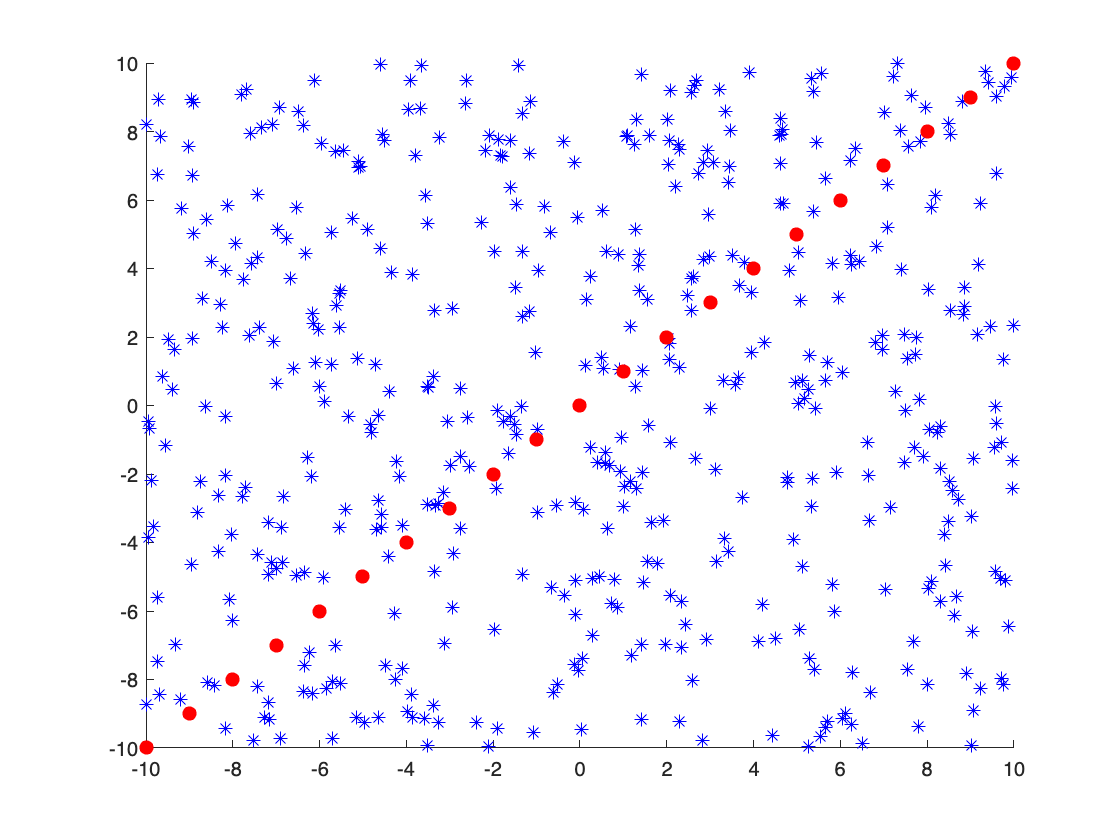
\includegraphics[width=.9\linewidth]{figures/clutter.intro.1.png}
   \caption{Real measurements from some object are shown as red dots. Clutter measurements are displayed as blue asterisks.}
  \label{fig:clutter-intro:1}
\end{subfigure}\hfill
\begin{subfigure}[t]{.45\textwidth}
  \centering
  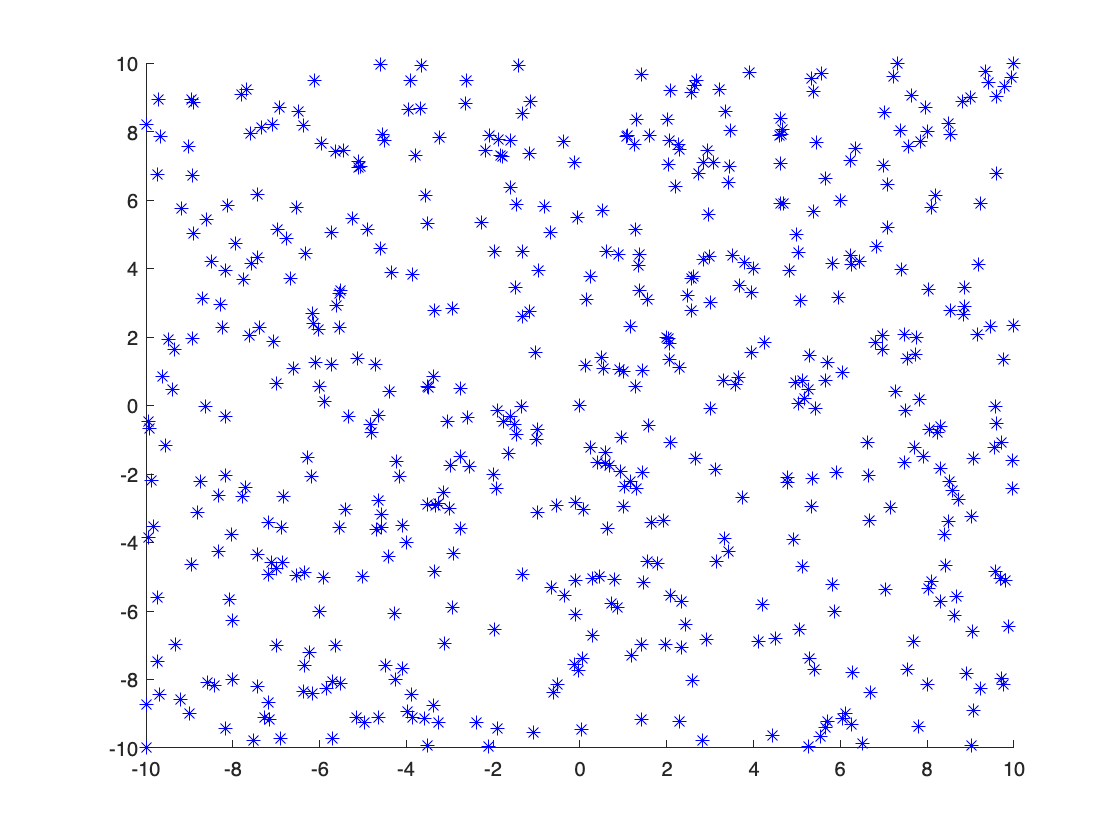
\includegraphics[width=.9\linewidth]{figures/clutter.intro.2.png}
  \caption{Both real measurements and clutter measurements are shown as blue asterisks.}
  \label{fig:clutter-intro:2}
\end{subfigure}
\caption[Measurements in clutter.]{Measurements in clutter. In this Figure, we indicate the clutter problem. When a sensor generates measurements, some of them may be clutter measurements, and there is no easy way to distinguish which data points come from a real object and which are noise.}
\label{fig:clutter-intro}
\end{figure}

The uncertainty in distinguishing between real measurements and clutter has led to the development of many methods for addressing this problem. The main idea behind these methods is that, since we have no information about which measurements come from targets and which are clutter, we should consider all measurements at each time step as coming from a target. This involves creating all possible assignments between measurements and targets and then evaluating the probability of each such assignment. In other words, we evaluate the possibility that a given measurement comes from a specific target according to its motion model. If the measurement is too far from the target, the probability of such an assignment will be lower than that of an assignment with a measurement that is close to the predicted state. These assignments are referred to as \textit{association hypotheses}. In the following subsection, we will provide a brief overview of various target tracking methods and approaches. But before doing so, we will outline the main assumptions of multi-target tracking (MTT).

    \section{Overview of target tracking methods}\label{sec:tt-overview}
        There are multiple filters that use association hypotheses. For single-target tracking, when the maximum number of targets is fixed to one, in Gaussian-linear scenarios the Probabilistic Data Association (PDA) filter can be utilized \cite{bar-shalomProbabilisticDataAssociation2009}. At each time step, this filter creates new hypotheses for all possible data associations and creates a joint posterior distribution after at the update step. Each hypothesis is assigned with a weight that reflects the likelihood that it actually originates from the target. Next, the resulting Gaussian mixture is reduced to only one Gaussian that represents the posterior state of the target. Both Gaussian mixtures and the reduction techniques will will be discussed later in this work.

This PDA filter is conceptually very simple and straightforward, but it may be too simple for many real-world scenarios, particularly when there are multiple targets present that are too close to each other to be tracked by multiple instance of the PDA filter. This is addressed in the extension and the resulting filter is named the Joint Probabilistic Data Association (JPDA) filter \cite{bar-shalomMultitargetmultisensorTrackingPrinciples1995}. It can handle multiple targets all at once but only when the number of targets is known in advance. The main idea behind this filter is that at each time step it creates all possible measurement-to-target association hypotheses, and, for each target, it creates a joint probability from all partial probabilities computed for each measurement. The series of such probabilities create tracks, and the track with the highest probability is considered the real track of the object. Because of the way how hypotheses are calculated, the JPDA filter is computationally much more expensive than the PDA filter. Moreover, if tracks get too close to each other, this filter shows the problem called the track coalescence—when tracks of two targets merge into one track.

Both PDA and JPDA filters are single-scan methods, which means they process only one set of measurements at a time. Compared to single-scan methods, there exist multi-scan methods that compute probabilities of tracks based on the history of all measurements, in a hierarchical manner. This way of calculating posterior probabilities leads to significant improvements in tracking accuracy, since the filter takes into consideration the whole history of the object movement. The classical example of a multi-scan filter is Reid's Multiple Hypothesis Tracker (MHT), also known as the hypothesis-oriented MHT (HO-MHT) \cite{reidAlgorithmTrackingMultiple1979}. This filter is similar to the way it computes probabilities; however, the calculation of the probability of each association hypothesis incorporates the probability of the parent hypothesis from the previous time step, thus creating a hypothesis tree at each filter cycle. The number of hypotheses is therefore multiplied by the number of new measurements at each step, and the total number of association hypotheses grows exponentially. Efficient implementations of the recursive HO-MHT include advanced techniques on how to prune the number of less probable hypotheses at each time step \cite{coxEfficientImplementationReid1996}.

The computational complexity of Reid's MHT has led to modifications in the way hypotheses are created. Instead of generating new hypotheses for all parent hypotheses at each time step, we can create several sequences of the best associations for several time steps in the past and compute new hypothesis probabilities for those hypotheses only. This reduction in the computational complexity avoids the need to compute all possible branches in the hypothesis tree. Moreover, it allows for efficient implementation techniques like look-up tables, and there is no recursion in the computation of new hypotheses. This algorithm is known as the track-oriented MHT (TO-MHT) \cite{werthmannStepbystepDescriptionComputationally1992}. As a modification of Reid's MHT, TO-MHT is also a multi-scan method, but instead of recursively evaluating all possible hypotheses, it processes all hypotheses at once.

The way both variants of MHT handle track hypothesis initialization and the propagation of association hypotheses over time allows ``the MHT approach inherently handle initiation and termination of tracks, and hence accommodate an unknown and time-varying number of targets'' \cite{voMultitargetTracking2015}. However, because the number of hypotheses grows exponentially, hypothesis reduction techniques should be used, and the pruning of hypotheses with low probabilities should be relatively aggressive. This makes MHT a strong algorithm but with higher computational requirements.

The JPDA filter and the MHT are two approaches for handling multiple targets in a scene. However, there is one alternative approach that is conceptually very different from both methods, which utilizes an abstract mathematical concept called Finite-Set Statistics (FISST) \cite{mahlerStatisticalMultisourcemultitargetInformation2007}. We will dedicate several next sections to explaining what FISST is, introducing the main theoretical assumptions of the multiple target tracking problem, and then discussing the main building blocks of the PHD filter.

    \section{Random Finite Sets}\label{sec:fisst}
        We have discussed one possible approach for evaluating the uncertainty between targets and measurements in multi-target tracking. Filters such as JPDA or MHT, in both variants, use a hypothesis-based approach where at each time step, a set of hypotheses is created to map all possible associations between new measurements and existing targets. However, these approaches do not model the uncertainty of the number of targets themselves. At any given moment, new targets may appear or disappear from the field of view, and the filters should be able to estimate tracks for every target.

To illustrate this point, let us consider the scenario of a common surveillance camera tracking people in a large mall. At every moment, people enter the area covered by the camera, cross it, and then leave the area. The number of people can vary greatly at different times of the day or on different days of the week, and there is no simple solution for estimating the number of mall visitors at every moment.

In the JPDA filter, the number of hypotheses is assumed to be known in advance, which is a rare case in real-world applications. In the MHT approach, object appearance events can be modeled by assuming that if two or more measurements have a high probability of being assigned to one target, this is probably because the number of objects in the vicinity of the target is greater than one. However, these approaches are not systematic nor optimal, and the exact estimation of the number of targets is rather a side effect \cite{challaFundamentalsObjectTracking2011}.

This problem led to the development of the Random Finite Sets (RFSs) theory, a completely new approach to multi-target tracking. At each time step, a collection of objects that are present in the field of view of a sensor is modeled as a random finite set. Generally, a set is a collection of distinct objects without a specific order of the elements. In an RFS, the number of objects is only known to be finite, but the exact cardinality, or the number of elements in the set, is modeled using some probability distribution. Moreover, all elements in the set are probability distributions. Therefore, RFSs are random variables that model the uncertainty of every state and the number of states as a single entity. An outcome, or a realization, of such a random variable is a fixed set with an exact state, and measurements are considered to be outcomes of the unknown internal state.

The RFS concept led to the development of a new branch in statistics called Finite Sets Statistics (FISST). In FISST, sets are random variables that have their probability distributions and probability density functions. Furthermore, FISST allows the use of RFSs for Bayesian inference, which leads to the need for defining basic algebraic operations on sets, such as integrals and derivatives. As we will soon see, the mathematics behind it becomes complex, and one way to simplify the notation is the introduction of a new way of expressing relations. This concept, called probability generating functionals (p.g.fls), significantly simplifies the notation in FISST. Unfortunately, the underlying level of mathematical abstraction becomes much more difficult to understand.

In this section, we will give a formal definition for a random finite set and also define the main formulas that are needed to understand the logic behind FISST and use it to infer the PHD filter. In this work, we will use standard notation that does not use p.g.fls. However, the reader may refer to the original work in \cite{mahlerMultitargetBayesFiltering2003} to learn about these concepts.

        \subsection{RFS formal definition}\label{sec:rfs-definition}
            As we mentioned earlier, random finite sets allow us to model object states and the cardinality of the set as a single random variable. At each time step $k$, we have a set of object states with cardinality $n_k$. We also assume that states are vectors from some space, and without loss of generality, we assume that this space is $\mathbb{R}^n$. Formally, for every time step $k$, we have vectors ${\vecat{x}{k}^{1}, \ldots, \vecat{x}{k}^{n_k}}$, where $\vecat{x}{k}^{i} \in \mathbb{R}^d$ for $\forall i$ and $\forall k$. We define the random finite set as follows:

\begin{definition}[Random finite set]
    Let $k$ be a time step and ${\vecat{x}{k}^{1}, \ldots, \vecat{x}{k}^{n_k}}$ be vectors from $\mathbb{R}^d$, where $n_k$ is a random number with a known distribution. Then, $\Xi_k \subseteq \mathbb{R}^d$ is a random finite set with cardinality $|\Xi_k| = n_k$, and $X_k = \{\vecat{x}{k}^{1}, \ldots, \vecat{x}{k}^{n_k}\}$ is called a realization of the RFS.
\end{definition}


It should be noted that the cardinality equal to zero is also valid, and in that case, the realization of an RFS is an empty set, i.e., $X_k = \emptyset$.

As we already know, RFSs are random variables, and we need an analogous mechanism as for classical random variables defined on vectors that allows us to describe the behavior of the RFS. For vector-based random variables, we have cumulative distribution functions and their first-order derivatives probability density function. The analogy to a cdf for a random finite set is called the \textit{belief mass measure} and is defined as follows:

\begin{definition}[Belief mass measure]
    Let $\Xi \subseteq \mathbb{R}^d$ be a random finite set, and $\mathcal{S} \subseteq \mathbb{R}^d$ be some region of the set space. The belief mass measure $\beta_\Xi$ of $\Xi$ is defined as:

    \begin{equation}
        \beta_\Xi(\mathcal{S})
        = \Pr{\Xi \subseteq \mathcal{S}}
        = \int_\mathcal{S} p_\Xi(X)\delta X,
    \end{equation}

    where $p_\Xi$ is a FISST density function, also called the multi-target pdf, and $\int_\mathcal{S} p_\Xi(X)\delta X$ is a set integral over all sets $X \subseteq \mathcal{S}$.
\end{definition}

In this work, we do not include the formal proof that $p_\Xi$ is indeed a pdf, i.e., $p_\Xi(X)$ for all $X$ and $\int_{\mathbb{R}^d} p_\Xi(X)\delta X = 1$. However, the reader may refer to the standard reference on FISST \cite{mahlerStatisticalMultisourcemultitargetInformation2007} to see the proofs. Here, we only emphasize that this function is a pdf for RFSs and it captures both the cardinality of a set and the distribution over elements in the set.

        \subsection{Set integral and the convolution formula}\label{sec:rfs-integral-convolution}
            In the definition above, we have used an integral on sets. For a set-valued function $f$, it is defined as:

\begin{equation}\label{eq:set-integral}
    \int_\mathcal{S} f(X) \delta X =
        \sum_{n=0}^{\infty} \frac{1}{n !}
        \int_{\mathcal{S} \times \ldots \times \mathcal{S}}
            f\left(\left\{\mathbf{x}^1, \ldots, \mathbf{x}^n\right\}\right) \mathrm{d} \mathbf{x}^1 \ldots \mathrm{d} \mathbf{x}^n.
\end{equation}

We can build the intuition for the set integral by understanding what integrated values really are. When we compute an integral over real values, we, in simple words, compute the value of the integrand for all possible values. The set integral is conceptually the same, however, the integrated value is a random set and there are two variables incorporated--the cardinality of the set, and the values. That means, that we sum up the function values for all possible cardinalities, from the empty set until infinity, and all possible elements in the set. The term $\frac{1}{n !}$ refers to the fact that for any two values $a, b$, sets $\{a, b\}$ and $\{b, a\}$ are equal, because sets are invariant to order. That means that any permutation of elements in the set leads to the same set, and the number of possible permutations is equal to $n!$.

The set integral is important for computing the posterior distribution in Bayesian inference. The Chapman-Kolmogorov equation is defined the same way for RFSs, as we will see later in this section, and it uses the total probability theorem where we compute the integral over all states from the previous time step. In case when the state is represented by a random set, the set integral is used.

In addition to the set integral, we are often interested in basic operations on sets, like union or intersection. For instance, if we have two random finite sets with two different distributions, what is the distribution of their union? To answer this question and to build the intuition, we shall return to a simpler case, discrete-valued random variables.

If we have two integer-valued random variables $X, Y$ with pmfs $p_X(x)$ and $p_Y(y)$, respectively, and their sum $Z = X + Y$, the probability that a realization of $Z$ is equal to the exact value $z$ is described using the so-called convolution formula:

\begin{equation}
    \Pr{Z = z} = \sum_{v = -\infty}^{+\infty} p_X(v) p_Y(z - v).
\end{equation}

The main idea behind the convolution is simple: we have an infinite number of possibilities how we can sum up two values and get the result equal to $z$. If we take a value $v$, then the second value is $z-v$, for all $v$. And the result is obtained by summing the probabilities of this pair of numbers.

The convolution over sets has the same idea, where we sum over all possible pairs of values that add up to a particular value. If $\Xi$ and $\Gamma$ are two random finite sets with multi-object probability density functions $p_\Xi(X)$ and $p_\Xi(Y)$, and $\Sigma = \Xi \cup \Gamma$, the probability that a realization of $\Sigma$ equals to the exact set $X$ is:

\begin{equation}
    p_\Sigma(Y) = \sum_{X \subseteq Y} p_\Xi(X) p_\Gamma(Y \setminus X),
\end{equation}

Simply speaking, we take some values (or none at all) from $X$ and create a set $Y$ containing these values, and the rest are assigned to the other set, $Y \setminus X$. Then, the probability of this assignment is evaluated and we take the sum of probabilities of all such assignments. Having understood the main concept, we are ready to define the set convolution for general cases.

\begin{definition}[Set convolution]\label{def:rfs-convolution}
    Let $\Xi$ be a random finite set and $\Xi_1 \cup \ldots \cup \Xi_n = \Xi$ be statistically independent subsets with multi-target probability density functions $p_{\Xi_1}(X), \ldots, p_{\Xi_n}(X)$, respectively. The multi-target pdf for $\Xi$ is then defined as:

    \begin{equation}
        p_\Xi(Y) = \sum_{X_1 \uplus \ldots \uplus X_n = Y} \prod_{i=1}^{n} p_{\Xi_i}(X_i),
    \end{equation}
    
    where the expression $X_1 \uplus \ldots \uplus X_n = Y$ represents the union of mutually disjoint (and possibly empty) subsets of $Y$ such that $X_1 \cup \ldots \cup X_n = Y$ \cite[385--386]{mahlerStatisticalMultisourcemultitargetInformation2007}.
\end{definition}

The convolution formula is a fundamental concept in FISST and multi-target tracking. In many filters, like, for instance, the Poisson Multi-Bernoulli Mixture filter \cite{garcia-fernandezPoissonMultiBernoulliMixture2018}, we model existing targets as a Bernoulli RFS, and the clutter as the Poisson RFS. Measurements at every time step contain a random permutation of true measurements and clutter, and in order to calculate the posterior density we model them as a union of two RFSs. The PHD filter, the filter covered in detail later in this work, also uses unions of several RFSs.

Last but not least, we should define the expected value of a RFS pdf and the cardinality distribution. The expected value is defined in almost the same way like for vector- or scalar-valued pdfs, however, there is one important difference, as the sum of RFSs is not defined, the average is not defined too, and we cannot calculate the expected value directly. However, if we define a function that maps a RFS into a space where the addition is defined, we can compute the expected value using this formula:

\begin{definition}[Expected value of a multi-target pdf]
    Let $\Xi$ be a RFS and $p_\Xi(X)$ be its multi-target pdf. Let $f: \mathcal{F}(D) \rightarrow \mathbb{R}$ be some function that maps a RFS into a real number\footnote{$\mathcal{F}(D)$ is a special function that creates a so-called power set, or all possible subsets of the set $D$.}. Then, the expected value is defined as follows:

    \begin{equation}
        E[f(\Xi)] = \int f(X)p_\Xi(X) \delta X
        = \sum_{n=0}^\infty \frac{1}{n !}
        \int f(\{\mathbf{x}^1, \ldots, \mathbf{x}^n\}
        p_\Xi(\{\mathbf{x}^1, \ldots, \mathbf{x}^n\}
        \mathrm{d}\mathbf{x}^1 \ldots \mathrm{d}\mathbf{x}^n.
    \end{equation}
\end{definition}

The expected value of a multi-target pdf is used when calculating the Chapman-Kolmogorov equation for RFSs describe in Section \ref{sec:bayes-filter-rfs}.

The cardinality distribution of a random finite set is a discrete distribution that has the probability mass function describing the probability of the set having the exact number of elements. 

\begin{definition}[Cardinality distribution of a RFS]
    Let $\Xi$ be a RFS and $p_\Xi(X)$ be its multi-target pdf and let the Kronecker delta function be denoted $\delta_y$ defined by:

    \begin{equation}
        \delta_y = \begin{cases}
            1, & \textup{if } y = 0, \\
            0, & \textup{otherwise}.
        \end{cases}
    \end{equation}
    
    Then, the cardinality pmf is defined as:

    \begin{align}
        \Pr{|\Xi| = k}
        &= E[\delta_{k - |\Xi|}] \\
        &= \sum_{n=0}^\infty \frac{1}{n !}
        \int \delta_{k - n}
        p_\Xi(\{\mathbf{x}^1, \ldots, \mathbf{x}^n\}
        \mathrm{d}\mathbf{x}^1 \ldots \mathrm{d}\mathbf{x}^n \\
        &= \frac{1}{k !}
        \int p_\Xi(\{\mathbf{x}^1, \ldots, \mathbf{x}^k\}
        \mathrm{d}\mathbf{x}^1 \ldots \mathrm{d}\mathbf{x}^k.
    \end{align}
\end{definition}

Before we proceed to the use of random finite sets in Bayesian inference and multi-target tracking, we should describe several known RFSs and their pdfs. In the next sections, we will describe set distributions that are already known to us: the Bernoulli RFS and the Poisson RFS. The latter has a direct relation to the important mathematical concept used in target-tracking, the point processes.

        \subsection{Bernoulli and Poisson RFS}\label{sec:bernoulli-poisson-rfs}
            The Bernoulli random finite sets is one of the simplest and straightforward RFS pdfs. Recall that the Bernoulli distribution is a discrete distribution that models the probability of the positive outcome. In multi-target tracking, Bernoulli RFSs are used to model the existence of one object. That is, the cardinality distribution takes values either one or zero (either an object exists or not) with some probability $r$. The state distribution of the object can be arbitrary. Formally, the Bernoulli RFS is defined as follows:

\begin{definition}[Bernoulli RFS]
    Let $\mathbf{x}$ be a random variable with the pdf $p(\mathbf{x})$, and let $0 \leq r \leq 1$ be some number. Then, the Bernoulli RFS $\Xi$ has the following pdf:

    \begin{equation}
        p_\Xi(X) =
        \begin{cases}
            1 - r & \textup{if } X = \emptyset, \\
            r p(\mathbf{x}) & \textup{if } X = \{\mathbf{x}\}, \\
            0 & \textup{otherwise}.
        \end{cases}
    \end{equation}

    \noindent The cardinality of the Bernoulli RFS has the Bernoulli distribution, that is:

    \begin{equation}
        \Pr{|\Xi| = k} = \begin{cases}
            1 - r & \textup{if } k = 0, \\
            r & \textup{if } k = 1, \\
            0 & \textup{otherwise}.
        \end{cases}
    \end{equation}
\end{definition}

The Poisson RFS is also a widely used multi-target pdf. It is commonly used to model clutter, since it has a parameter $\lambda$ that represents the intensity, or the expected number of noise measurements.

\begin{definition}[Poisson RFS]
    Let $\mathbf{x}$ be a random variable with the pdf $p(\mathbf{x})$, and let $\lambda(x)$ be the intensity function\footnote{Note that the intensity function can be an arbitrary function depending on the domain of the Poisson RFS.}. Then, the multi-target pdf of the Poisson RFS $\Xi$ is:

    \begin{equation}\label{eq:poisson-rfs-pdf}
        p_\Xi(X) = \exp\left(-\int \lambda(\mathbf{x}) \mathrm{d}\mathbf{x}\right)
        \prod_{\mathbf{x} \in \Xi} \lambda(\mathbf{x}).
    \end{equation}

    \noindent The cardinality pmf of the Poisson RFS is Poisson-distributed with the rate parameter $\hat{\lambda} = \int \lambda(\mathbf{x}) \mathrm{d}\mathbf{x}$ is the following:

    \begin{equation}
        \Pr{|\Xi| = k} = \operatorname{Poisson}(k; \hat{\lambda}).
    \end{equation}
\end{definition}

Intuitively, the Poisson RFS pdf represents the probability of observing any finite set of objects anywhere in the area, given that objects appear over it independently. In contrast to the Bernoulli distribution, the Poisson RFS cannot be used to model the target existence, since there is no way to limit the cardinality. However, when the location of the points is random through the whole surveillance area, and the number of these points is Poisson-distributed, the Poisson RFS is a good choice.

Both the Bernoulli RFS and the Poisson RFS are examples of so-called point processes, also called the Bernoulli process and the Poisson Point Process (PPP), respectively. Generally, a point process is a mathematical model that describes the random spatial distribution of points. In target tracking, point processes model various events, such as object appearance, disappearance, or movement. In particular, the PDF filter uses the PPP to model clutter, where clutter measurements are independent and appear uniformly over the whole surveillance area. For more information about point processes, the reader is referred to the classical textbook on the topic \cite{streitPoissonPointProcesses2010}.

        \subsection{Bayes filter in terms of RFSs}\label{sec:bayes-filter-rfs}
            In Section \ref{sec:bayes-filter}, we have discussed the prediction step, also known as the Chapman-Kolmogorov equation, and the update step in term of state vectors and motion and measurement models. In this section, we will derive similar formulas for Bayesian inference in the context of random finite sets.

Since RFS pdfs are indeed densities, as we discussed in Section \ref{sec:rfs-definition}, the recursive relations for RFS have the same form, however, densities are multi-target densities that catch the motion of all objects at once, and arguments are sets.

\begin{theorem}[The prediction step for RFS]{theorem:bayes-filter-predict-rfs}
    Given sets of measurements $Z_{1:k-1} = \{Z_1,\allowbreak Z_2, \ldots, Z_{k-1}\}$, the current state RFS $X_{k-1}$, the multi-target transition density $f_{k|k-1}(X_k | X_{k-1})$, and the multi-target posterior density from the previous time step $p_{k-1}\left({X}_{k-1} | {Z}_{1:k-1}\right)$, the prediction step of the Bayes filter for RFSs is computed as follows:

    \begin{equation}
        p_{k|k-1}\left({X}_k | {Z}_{1:k-1}\right)
        = \int
            f_{k|k-1}\left( {X}_k | {X}_{k-1} \right)
            p_{k-1}\left( {X}_{k-1} | {Z}_{1: k-1} \right)
            \delta {X}_{k-1}.
    \end{equation}
\end{theorem}

\begin{theorem}[The update step for RFS]\label{theorem:bayes-filter-update-rfs}
    Given the predicted density $p_{k|k-1}\left({X}_k | {Z}_{1:k-1}\right)$, the observed set of measurements $Z_k$ and the multi-target likelihood $g_k(Z_k | X_k)$, the update step of the Bayes filter for RFS is computed as follows:
    
    \begin{align}
        p_{k}\left({X}_k | {Z}_{1: k}\right)
        &= \frac{
            g_k\left({Z}_k | {X}_k\right) p_{k|k-1}\left({X}_k | {Z}_{1: k-1}\right)
        }{
            \int g_k\left({Z}_k | X\right) p_{k|k-1}\left(X | {Z}_{1: k-1}\right) \delta X
        } \\
        &\propto g_k\left({Z}_k | {X}_k\right) p_{k|k-1}\left({X}_k | {Z}_{1: k-1}\right).
    \end{align}
\end{theorem}

Note that the multi-target transition density is not the same motion model that we used before. The same applies for the multi-target likelihood that plays the role of the measurement model but is a completely different relation. The transition density captures the motion of all objects in a set all at once, including the birth (appearance) of new objects, and the death (disappearance). The likelihood, on the other hand, models the transition from a set of object states to probable measurements. Arguments of both are now sets, and explicit forms can be derived from motion and measurement models using FISST. These derivations along with formal proofs of the Bayesian recursion defined above can be found in \cite{mahlerMultitargetBayesFiltering2003}.

Even though the relations look similarly on the first glance, the underlying mathematics differs drastically. In comparison to the single-object tracking, states now represent the distribution of all objects simultaneously. Moreover, the multi-target transition density now captures much more information: not only it describes the transition of objects that are already in the current state set, but also the behavior of the change of the cardinality of the set. In the next section, we will explore how these relations can be applied to address the multi-target tracking problem. We will also examine the assumptions that must be made in order to develop Bayes filters based on FISST.

        \subsection{Multi-target tracking standard model}\label{sec:mtt-standard-model}
            We have now reached the final fundamental theoretical section where we will give a formal definition to the multi-target tracking problem. We have already mentioned that the multi-target transition density includes more than a standard motion model; more specifically, it describes not only the dynamics of all underlying objects in the current state set but also the birth and death of objects. In this section, we will cover in detail how new objects are born, the survival probability, and how we can model clutter. These concepts are fundamental for building the PHD filter.

Let $\mathcal{X}$ be the state space and $\mathcal{Z}$ be the measurement space. Elements of $\mathcal{X}$ are state vectors of one object, and $\mathcal{Z}$ contains elements that are measurement vectors. For instance, for the CV model covered in Section \ref{sec:cv-model}, the state space is $\mathbb{R}^4$, and the measurement space is $\mathbb{R}^2$. Assume that at time $k$, the number of targets is $M(k)$. This number varies at every time step since new targets may appear or disappear. The \textit{multi-target state set} at time $k$ is therefore $X_k = \{\svecat{x}{k}{1}, \ldots, \svecat{x}{k}{M(k)}\} \in \mathcal{F}(\mathcal{X})$. Also, at every time step, we get a measurement set. Let us denote the number of measurements at time $k$ as $N(k)$. Thus, the \textit{multi-target observation set} at time $k$ is $Z_k = \{\svecat{z}{k}{1}, \ldots, \svecat{z}{k}{M(k)}\} \in \mathcal{F}(\mathcal{Z})$. The order of elements in both sets is not significant. The measurement set contains not only those measurements that come from real objects but also clutter, and those noise vectors are indistinguishable from those coming from targets. The goal of the multi-target tracker is to filter out the clutter and to find the best mapping between the objects and measurements.

Existing targets either move according to their underlying dynamics model to the next state or die (disappear). The transition from the state $\vecat{x}{k-1} \in X_{k-1}$ to $\vecat{x}{k} \in X_{k}$ happens according to the specified motion model of the target, $f_{k|k-1}(\vecat{x}{k} | \vecat{x}{k-1})$. The death of one target happens with the probability $1 - P_{S,k}(\vecat{x}{k-1})$, and the target survives with the probability $P_{S,k}(\vecat{x}{k-1})$. This probability is referred to as the \textit{survival probability}. In terms of RFSs, the survival of a target with the state $\vecat{x}{k-1}$ is modeled using the survival function on an RFS $S_{k|k-1}$:

\begin{equation}
    S_{k|k-1}(\vecat{x}{k-1}) = \begin{cases}
        \{\vecat{x}{k}\}, & \text{if the target survives}, \\
        \emptyset, & \text{otherwise}.
    \end{cases}
\end{equation}

At every time step, new targets may appear (be born). The birth process is considered spontaneous, and the exact distribution of newborn targets is domain-dependent. In general, the target birth distribution includes the location where new targets appear and their intensity. For instance, the birth process may be modeled by the Poisson Point Process, as in \cite{garcia-fernandezPoissonMultiBernoulliMixture2018}, or the Gaussian mixture for Gaussian-linear cases, as we will later see. In terms of FISST, the birth of new targets is a random set $B_{k|k-1}(\cdot)$ that contains newly born targets when the transition from the multi-target state $X_{k-1}$ to the state $X_{k}$ occurs.

Given that we have the relations for both the transition from the current multi-target state and the birth set, and assuming that the multi-target state at the previous time step $k-1$ is $X_{k-1}$, we can derive the following expression for the multi-target state $X_k$, assuming that the survival and birth processes are independent of each other\footnote{
Note that, in addition to the survival set and the birth process, \cite{voGaussianMixtureProbability2006} assumes the existence of the spawning process $\bigcup_{\zeta \in X_{k-1}} B_{k|k-1}(\zeta)$, i.e., that the existing targets may randomly spawn new targets in the same location. While this is important in the defense area, such as when a fighter takes off from an aircraft carrier, we do not include this process in this work. Fundamentally, the underlying mathematics does not change.}:

If we apply the convolution formula from Definition \ref{def:rfs-convolution}, and introduce the simplified notation $S_{k|k-1}^i = S_{k|k-1}(\svecat{x}{k-1}{i})$, the complete multi-target motion model $f_{k|k-1}(X_k | X_{k-1})$ has the following form:

\begin{equation}
    f_{k|k-1}(X_k | X_{k-1}) = 
    \sum_{
        \Gamma_k \uplus S_{k|k-1}^1 \ldots \uplus S_{k|k-1}^{M(k-1)} = X_{k-1}
    }
    \gamma_k(\Gamma_k)
    \prod_{i=1}^{M(k-1)}
    s_{k|k-1}(S_{k|k-1}^i | \svecat{x}{k-1}{i}),
\end{equation}

\noindent where $\gamma_k(\cdot)$ is the intensity function of the birth process, which can be a Poisson RFS pdf defined in Equation \ref{eq:poisson-rfs-pdf}, and $s_{k|k-1}(S_{k|k-1}^i | \svecat{x}{k-1}{i})$ is the multi-target transition density defined as:

\begin{equation}
    s_{k|k-1}(S_{k|k-1}^i | \svecat{x}{k-1}{i}) = \begin{cases}
        P_{S,k}(\svecat{x}{k-1}{i})
            f_{k|k-1}(\vecat{x}{k} | \svecat{x}{k-1}{i}) & \text{if } S_{k|k-1}^i = \{\vecat{x}{k}\}, \\
            1 - P_{S,k}(\svecat{x}{k-1}{i}), & \text{if } S_{k|k-1}^i = \emptyset.
    \end{cases}
\end{equation}

The multi-target measurement model, or the multi-target likelihood, also consists of several parts. At time $k$, a target may generate a new measurement with probability $P_{D,k}(\vecat{x}{k})$, and there will be a misdetection with probability $1 - P_{D,k}(\vecat{x}{k})$. A measurement is generated according to the measurement model, $g_{k}(\vecat{z}{k} | x_{k})$. Thus, the measurement RFS at time $k$ is:

\begin{equation}
    \Theta_k(\vecat{x}{k}) = \begin{cases}
        \{\vecat{z}{k}\}, & \text{if target is detected}, \\
        \emptyset, & \text{otherwise}.
    \end{cases}
\end{equation}

Additionally, at every time step, false measurements are generated by a sensor. The RFS with clutter is denoted as $K_k$. Both $\Theta_k(\vecat{x}{k})$ and $K_k$ create the multi-target measurement set $Z_k$:

\begin{equation}
    Z_k = K_k \cup \left[ \bigcup_{\vecat{x}{k} \in X_k} \Theta_k(\vecat{x}{k}) \right].
\end{equation}

As we did for the multi-target transition density, we denote $\Theta_k^i = \Theta_k(\svecat{x}{k}{i})$ and apply the set convolution formula to get the multi-target measurement likelihood:

\begin{equation}
    p_k(Z_k | X_k) = \sum_{
        K_k \uplus \Theta_{k}^1 \ldots \uplus \Theta_{k}^{M(k)} = X_{k}
    }
    \kappa_k(K_k)
    \prod_{i=1}^{M(k)}
    \theta_{k}(\Theta_{k}^i | \svecat{x}{k}{i}),
\end{equation}

\noindent where $\kappa_k(K_k)$ is the clutter intensity function, which is often modeled as a Poisson RFS, and $\theta_{k}(\Theta_{k}^i | \svecat{x}{k}{i})$ is the multi-target measurement density defined as:

\begin{equation}
    \theta_k(\Theta_{k}^i | \svecat{x}{k}{i}) = \begin{cases}
        P_{D,k}(\svecat{x}{k}{i})
            g_k(\vecat{z}{k} | \svecat{x}{k}{i}), & \text{if } \Theta_{k}^i = \{\vecat{z}{k}\}, \\
            1 - P_{D,k}(\svecat{x}{k}{i}), & \text{if } \Theta_{k}^i = \emptyset.
    \end{cases}
\end{equation}

In general, multi-target trackers are built on top of several general assumptions about the problem. These assumptions form the Standard Model of Multi-target tracking \cite[311--313]{mahlerStatisticalMultisourcemultitargetInformation2007}. We will enumerate these assumptions, which summarize this section, in the following list:

\begin{enumerate}
    \item The clutter process is Poisson-distributed in time and uniformly distributed in space.
    \item The clutter process, target motions, and observations are statistically independent.
    \item The transition density and the measurement likelihood are Markovian, that is once $\vecat{x}{k-1}$ is known, then $\vecat{x}{k}$ is independent of $\vecat{x}{k-2}$, $\vecat{x}{k-3}$, etc.
    \item Existing targets survive from time $k-1$ to $k$ with the probability $P_{S,k}(\cdot)$ and move to the next state with the motion model $f_k(\vecat{x}{k} | \vecat{x}{k-1})$.
    \item A target generates a measurement with probability $P_{D,k}(\cdot)$ with the measurement model $g(\vecat{z}{k} | \vecat{x}{k})$.
    \item A target generates no more than one measurement at a time.
    \item The birth process is Poisson-distributed in time.
\end{enumerate}

The PHD filter also relies on these main assumptions. In the following sections, we present the PHD filter, which is based on the propagation of the first-order multi-target moment, or the PHD function, in time instead of the full posterior distribution. Next, we will derive relations for the Gaussian-linear case to get equations of the GM-PHD filter. Finally, we present the way how we can input additional information into the filter to get better tracking results.

    \section{The PHD filter}\label{sec:phd-filter}
        The Probability Hypothesis Density (PHD) filter is a popular approach to multi-target tracking, especially when the number of targets is unknown and varies over time. The general formulation of the filter was first introduced by Mahler \cite{mahlerMultitargetBayesFiltering2003} as a direct application of the probability hypothesis density function. The filter is based on finite set statistics (FISST), covered briefly in Section \ref{sec:fisst}, and works by propagating the first-order multi-target moment, or the PHD function, in time instead of the full posterior distribution. This greatly reduces the computational burden of the filter compared to traditional hypotheses-based methods such as the MHT filter.

In 2003, Vo proposed the sequential Monte Carlo implementation of the PHD filter \cite{voSequentialMonteCarlo2003}, known as the SMC-PHD filter. However, this implementation had several drawbacks, such as a high computational cost due to the large number of particles required for distribution approximation and the reliance on clustering techniques for state estimation. Later, in 2006, Vo and Ma introduced a closed-form solution for the Gaussian-linear case \cite{voGaussianMixtureProbability2006}, called the GM-PHD filter. For non-linear models, the authors suggested implementations that utilize non-linear Kalman filters, such as the Unscented Kalman Filter and the Extended Kalman Filter. The versions of the PHD filter with these linearization techniques were called UK-PHD and EK-PHD, respectively. The GM-PHD filter was a significant improvement over the SMC-PHD filter in terms of computational efficiency while still providing accurate estimates of the number of targets and their states. The GM-PHD filter is the main topic of this work.

% PHD assumptions: \cite[588--590]{mahlerStatisticalMultisourcemultitargetInformation2007}
        \subsection{The PHD function}\label{sec:phd-function}
            The probability hypothesis density (PHD) function is the first-order moment of a random finite set, also known as the \textit{intensity function}. Its value is the expected number of targets in a certain area of the target space. From Section \ref{sec:prob-distributions}, we know that the first-order moment is the expectation value, but what is the expectation value of a set? To answer this question, let us define the problem formally. The computations that follow are based on the original book by Mahler \cite[576--578]{mahlerStatisticalMultisourcemultitargetInformation2007}.

Let a random finite set be denoted by $\Xi$ with the multi-target probability distribution $p_\Xi(X)$, and the target space $\mathcal{X}$. The expected number of targets is, conceptually, the integral over all targets multiplied by the value of the probability density function for each state value. However, since summing over targets will not have any meaning in terms of the expected value, we introduce the delta function of a set:

\begin{equation}
    \delta_\Xi(\mathbf{x}) = \begin{cases}
        0, & \text{if } X = \emptyset, \\
        \sum_{\mathbf{w} \in X} \delta_\mathbf{w}(\mathbf{x}), & \text{otherwise},
    \end{cases}
\end{equation}

\noindent where $\delta_\mathbf{w}$ is the Dirac delta density centered at $\mathbf{w}$, the continuous-space analog of the Kronecker delta function mentioned in Definition \ref{def:cardinality-rfs}.

\begin{definition}[PHD function]\label{def:phd-function}
    Given a random finite set $\Xi$, where elements of $\Xi$ are from $\mathcal{X}$, with the multi-target density $p_\Xi(X)$, the expected value of the set $\Xi$ is defined as:

    \begin{equation}
        v_\Xi(\mathbf{x}) = E[\delta_\Xi(\mathbf{x})] = \int \delta_\Xi(\mathbf{x}) \cdot p_\Xi(X) \delta X.
    \end{equation}

    The function $v_\Xi(\mathbf{x})$ is also called the Probability hypothesis density (PHD) function.
\end{definition}

The PHD function is not a probability density function, that is, it is not normalized to integrate to one. The integral of the PHD function over some subspace $S$ yields the expected number of targets in this subspace:

\begin{equation}\label{eq:phd-func-integral}
    E[| \Xi \cap S |] = \int_S v_\Xi(\mathbf{x}) \mathrm{d} \mathbf{x}.
\end{equation}

This formulation prompts that the PDF function is an unnormalized multi-target probability density function with the normalization constant equal to the expected number of existing targets $\hat{N}$ over the whole space $\mathcal{X}$, i.e., $\hat{N} = \int_\mathcal{X} v_\Xi(\mathbf{x}) \mathrm{d} \mathbf{x}$. Therefore, the peaks of this distribution are the most probable locations of the tracked targets. The density evolves over time as targets move in space. An example of the PHD function is illustrated in Figure \ref{fig:phd-function}.

\begin{figure}
    \centering
    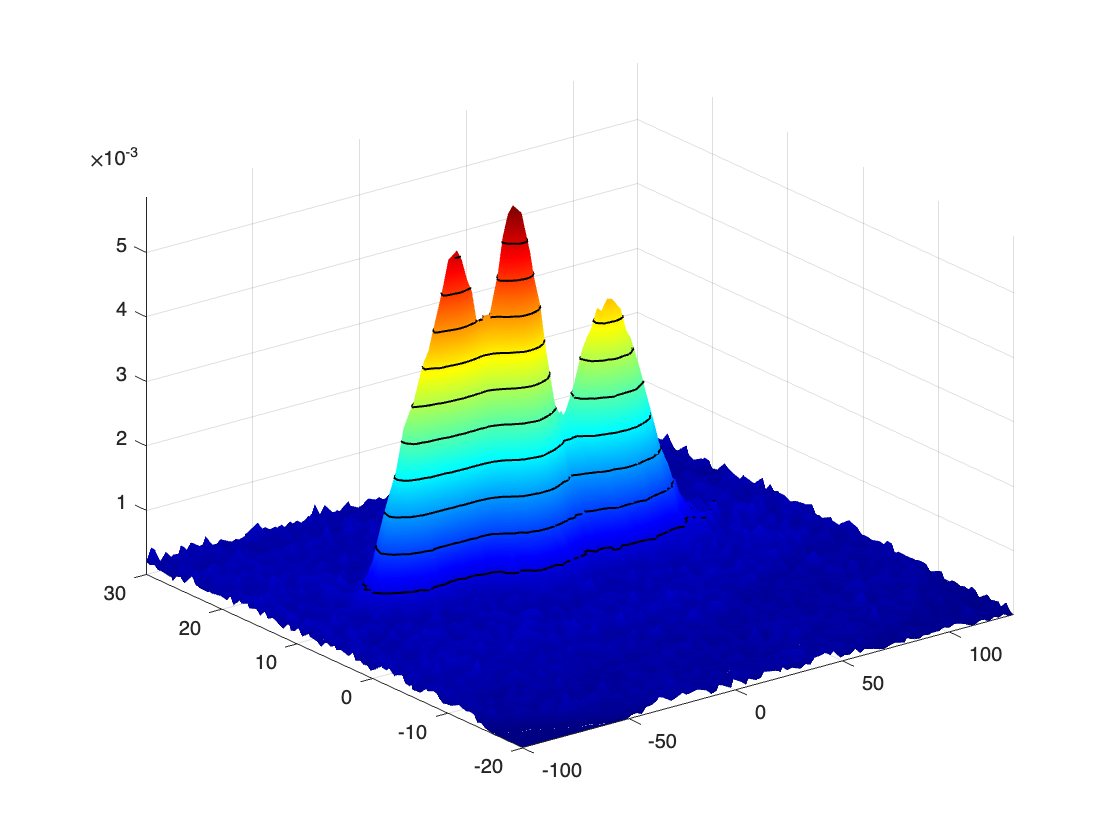
\includegraphics[width=.6\linewidth]{figures/phd-function.png}
    \caption[PHD function example]{An example of the PHD function. Three targets move in the 2D Euclidean space according to a CV model. Note that this function is not normalized, which means that the integral over the entire space is not equal to one. In this example, the expected number of targets in the space is approximately 3.2245, which can be inferred from the location of the corresponding peaks.}
    \label{fig:phd-function}
\end{figure}

The fact that the PHD function does not include normalization allows an efficient computation of this function in terms of the computational complexity. This fundamental property of the PHD function led to the development of the PHD filter. In the next section, we will define several assumptions of the PHD filter and define the predict-update cycle.

        \subsection{PHD filter formal definition}\label{sec:phd-filter-formal}
            We have defined the PHD function and mentioned that instead of propagating the full posterior density, the PHD filter propagates the first-order moment of the multi-target posterior state. In this section, we will describe the main assumptions of the PHD filter and derive the predict and update step equations in terms of the PHD function. It should be noted that while the PHD filter is a general concept, its implementation is specific to the problem domain. Later sections will provide the exact closed-form solution for Gaussian-linear problems.

The PHD filter relies on several general assumptions about the modeled problem. In addition to the standard assumptions, the PHD filter assumes:

\begin{enumerate}
\item Each target has a single-target motion model $f_k(\vecat{x}{k} | \vecat{x}{k-1})$.
\item Existing targets move to the next state with probability $P_{S,k}(\vecat{x}{k-1})$.
\item New targets are born with states from $X$ according to the multi-target birth likelihood $\gamma_k(X)$. The corresponding PHD of this likelihood is:
\begin{equation}
\gamma_k(\mathbf{x}) = \int \gamma_k({\mathbf{x}} \cup X) \delta X.
\end{equation}
\item Existing targets generate measurements according to the single-target Markovian measurement model $g(\vecat{z}{k} | \vecat{x}{k})$ with probability $P_{D,k}(\vecat{x}{k})$.
\item Clutter measurements are Poisson-distributed in time with the spatial distribution $\kappa_k(\vecat{z}{k})$.
\item The predicted multi-target distribution $p_{k|k-1}(\vecat{x}{k} | \vecat{z}{1:k-1})$ is a Poisson RFS.
\end{enumerate}

The last assumption is a simplification that allows to derive a closed form solution. A Poisson process assume that all targets are statistically independent, and such approximation is not that restrictive is the interactions between moving targets in negligible. In this work we do not include the spawning process, therefore, it can be shown that this requirement is satisfied \cite{voGaussianMixtureProbability2006}.

Both the prediction and the update follow the same rules we have derived in Section \ref{sec:bayes-filter-rfs}. It can be shown that the Chapman-Kolmogorov equation and the measurement correction step for the PHD filter, excluding target spawning, has the following form:

\begin{theorem}[The PHD recursion]
    Assuming that all requirements defined above hold, the PHD recursion has the following form:

    \begin{align}
        v_{k|k-1}(\vecat{x}{k} | Z_{1:k-1})
        &= \gamma_k(\vecat{x}{k-1}) + \int P_{S,k}(\vecat{x}{k-1}) f_{k|k-1}(\vecat{x}{k} | \vecat{x}{k-1}) v_{k-1}(\vecat{x}{k-1} | Z_{1:k-1}) \mathrm{d} \vecat{x}{k-1}, \\
        v_k(\vecat{x}{k} | Z_{1:k})
        &= \left[1-P_{D,k}(\vecat{x}{k})\right] v_{k|k-1}(\vecat{x}{k} | Z_{1:k-1}) \\
        &+ \sum_{\vecat{z}{k} \in Z_k} \frac{
            P_{D,k}(\vecat{x}{k}) g_k(\vecat{z}{k} | \vecat{x}{k}) v_{k|k-1}(\vecat{x}{k} | Z_{1:k-1})
        }{
            \kappa_k(\vecat{z}{k}) + \int P_{D,k}(\boldsymbol{\xi}) g_k(\vecat{z}{k} | \boldsymbol{\xi}) v_{k|k-1}(\boldsymbol{\xi} | Z_{1:k-1}) \mathrm{d} \boldsymbol{\xi}
        },
    \end{align}

    \noindent where $v_{k-1}(\vecat{x}{k-1} | Z_{1:k-1})$ is the posterior PHD function from the previous time step \cite{voGaussianMixtureProbability2006} \cite[588--591]{mahlerStatisticalMultisourcemultitargetInformation2007}.
\end{theorem}

Note that the computation of the posterior probability hypothesis density after the update does not include the set integral, which means that we do not need to compute all association hypotheses between measurements and states, decreasing the computational burden. It can be shown that the computational complexity of the PHD filter at every time step is $\mathcal{O}(mn)$, where $m$ is the number of measurements and $n$ is the number of current targets \cite[592]{mahlerStatisticalMultisourcemultitargetInformation2007}.

In the next section, we will provide the formulation of the PHD filter in terms of Gaussian-linear filtering and Gaussian mixtures. We will see that for such cases a closed-form solution exists, and there are no approximations required to compute the posterior PHD density.

        \subsection{The Gaussian Mixture PHD filter}\label{sec:gm-phd}
            The Gaussian Mixture Probability Hypothesis Density (GM-PHD) filter was proposed in 2006 by Vo and Ma in \cite{voGaussianMixtureProbability2006} as a closed-form solution for the Gaussian-linear case of the general PHD filter and quickly became popular. As mentioned in the previous section, the PHD filter does not propagate the full posterior distribution, which eliminates the need to compute hypothesis likelihoods between measurements and existing targets. Therefore, the resulting filter is not computationally expensive as hypotheses-oriented filters like the MHT filter or filters that are built on top of the FISST theory and utilize random finite sets and the convolution formula to compute the full posterior distribution at each time step.

In the GM-PHD filter, the posterior intensity function is described by a Gaussian mixture. The same applies to the initial prior distribution and birth components. The clutter is modeled using a Poisson Point Process. Both the prediction and update steps utilize the equations that were inferred in the previous section, and the target dynamics and the single-target measurement likelihood are modeled using the standard Kalman filter equations. In this section, we will give a formal definition of the GM-PHD filter along with the exact algorithm. All relations described in this section follow those provided in \cite{voGaussianMixtureProbability2006} with the addition of labels (or tags) for Gaussian components from \cite{clarkGMPHDFilterMultiple2006} to enable basic track management. It should be noted that the notation in this work is slightly modified to stay consistent with the notation given in previous sections. Moreover, as noted before, we assume that existing targets cannot spawn additional targets, so the independence of targets' dynamics is preserved.

            \subsubsection{Track maintenance}\label{sec:track-maintenance}
                In this section, we will briefly cover one of challenges in multi-target tracking, which is track maintenance and then we introduce the way how this challenge may be addressed in the GM-PHD filter. When an algorithm creates estimates of targets at each time step, these estimates cannot always be implicitly connected to those from previous time steps. If we require not only point estimates but also the trajectories of targets, we should use techniques to maintain identities of targets and to create associations between new measurements and these identities. Thus, the trajectory here refers to the collection of state estimates of a target in time. Generally, the track maintenance problem includes three disjoint sub-problems: track initialization, track confirmation and track deletion \cite{blackmanDesignAnalysisModern1999}. Track initialization refers to the creation of new tracks. A new track is initialized when a new measurement is received that cannot be assigned to any existing track. Since the measurement is not always the true measurement, the tentative track should be confirmed by receiving subsequent measurements that meet certain criteria. Different algorithm specify various different criteria depending on their internal logic. For instance, one way to confirm tracks is called the $M/N$ rule, which states that the track becomes confirmed if at least $M$ measurements out of $N$ subsequent updates should be assigned to the tentative track \cite[871]{blackmanDesignAnalysisModern1999}. Confirmed tracks create trajectories of objects and we need a way to terminate tracks that do not receive measurements anymore, for example, when a target leaves the field of view. Yet again, there are multiple different ways how to approach this problem, including restricting the maximum age of a track, or when the likelihood of target existence falls under some threshold \cite[243]{challaFundamentalsObjectTracking2011}.

Estimating tracks has several challenges that need to be addressed to implement an effective tracking algorithm. For example, the track loss occurs when a track is temporarily or permanently lost due to a missed detection or incorrect association between a measurement and some existing track. Wrong associations may also cause track swaps, when an algorithm swaps measurements from two or more targets moving closely to each other, and measurements generated by one target are assigned to a track of another, and vice versa. Closely moving targets may also create a so-called track coalescence, the situation when two tracks of different targets are merged into one track in the middle of trajectories of these two targets. For instance, the JPDA filter is known to suffer from track coalescence \cite{kropfreiterTrackCoalescenceRepulsion2021}.

Despite there are many advanced techniques how to maintain track, we choose a straightforward approach in this work for the implementation of the GM-PHD filter. Every Gaussian component receives a unique tag, or label, that identifies this component. When the algorithm generates state estimates, these tags are used to connect single-target estimates from different time steps and having the same label into one trajectory. The track is terminated when the Gaussian component with the tag assigned to this track is removed from the mixture. While this approach is intuitive and simple, in Chapter \ref{ch:results} we show that is shows good performance results.

            \subsubsection{GM-PHD recursion}\label{sec:gm-phd-recursion}
                Before we start to deduce all formulas of the GM-PHD filter, we should make several additional assumptions for the Gaussian-linear case in addition to the general ones given in Section \ref{sec:phd-filter-formal}:

\begin{enumerate}
    \item All targets have a Gaussian-linear single-target motion and measurement models, that is:

    \begin{align}
        f_{k|k-1}(\vecat{x}{k} | \vecat{x}{k-1}) &= \mathscr{N}\left(\vecat{x}{k}; \vecat{F}{k-1} \vecat{x}{k-1}, \vecat{Q}{k-1}\right), \\
        g_{k}(\vecat{z}{k} | \vecat{x}{k}) &= \mathscr{N}\left(\vecat{z}{k}; \vecat{H}{k}\vecat{x}{k}, \vecat{R}{k}\right),
    \end{align}

    \noindent where the detailed explanation of the meaning of $\vecat{F}{k-1}, \vecat{Q}{k-1}, \vecat{H}{k}, \vecat{R}{k}$ are given in Section \ref{sec:state-space}.
    
    \item Both the survival and detection probabilities are constant in time\footnote{A closed-form solution can be derived without this assumption, see Section III-E in \cite{voGaussianMixtureProbability2006}.}, that is, they do not depend on states:

    \begin{align}
        P_{S, k}(\vecat{x}{k-1}) &= P_{S, k},\\
        P_{D, k}(\vecat{x}{k}) &= P_{D, k}.
    \end{align}

    \item The birth intensity is modeled using a Gaussian mixture of the form:

    \begin{equation}\label{eq:gm-phd-birth-gm}
        \gamma_k(\vecat{x}{k-1}) = \sum_{i=1}^{J_{\gamma, k}} w_{\gamma, k}^{(i)}
        \mathscr{N}\left(\vecat{x}{k-1}; \vecat{m}{\gamma, k}^{(i)}, \vecat{P}{\gamma, k}^{(i)}\right),
    \end{equation}

    \noindent where $J_{\gamma, k}$ denotes the number of birth components, and $\vecat{m}{\gamma, k}^{(i)}$ and $\vecat{P}{\gamma, k}^{(i)}$ are the mean vector and the covariance matrix of each component. These are given as parameters and specified in advance according to the problem domain. Since this mixture is not a probability density by an intensity function, weights do not need to sum to one, and the weights $w_{\gamma, k}^{(i)}$ here represent the expected number of new targets that are expected to appear in a location centered at $\vecat{m}{\gamma, k}^{(i)}$.
\end{enumerate}

These assumptions form the basis for the Gaussian-linear PHD filter recursion formulas. Assuming these assumptions hold for a given problem, and by following the PHD filter recursion equations from Theorem \ref{theorem:phd-recursion}, we propose the following theorem:

\begin{theorem}[The GM-PHD filter prediction]\label{theorem:gm-phd-prediction}
    Given that the posterior intensity of the previous time step $v_{k-1}(\vecat{x}{k-1} | Z_{1:k-1})$ is a Gaussian mixture of the form:

    \begin{equation}
        v_{k-1}(\vecat{x}{k-1} | Z_{1:k-1}) = \sum_{i=1}^{J_{k-1}}
        \mathscr{N}\left(\vecat{x}{k-1}; \vecat{m}{k-1}^{(i)}, \vecat{P}{k-1}^{(i)}\right),
    \end{equation}

    \noindent where every Gaussian component has a unique tag or label assigned to it, which forms the set of tags:

    \begin{equation}
        T_{k-1} = \{ T_{k-1}^{(1)}, \ldots, T_{k-1}^{(J_{k-1})} \}.
    \end{equation}

    \noindent Then the predicted intensity at time $k$ is also a Gaussian mixture, defined as:

    \begin{equation}
        v_{k|k-1}(\vecat{x}{k} | Z_{1:k-1}) = \gamma_k(\vecat{x}{k}) + v_{S, k|k-1}(\vecat{x}{k}),
    \end{equation}

    \noindent where $\gamma_k(\vecat{x}{k})$ is given in Equation \ref{eq:gm-phd-birth-gm} and $v_{S, k|k-1}(\vecat{x}{k})$ is the PHD function of survived targets given by:

    \begin{align}
        v_{S, k|k-1}(\vecat{x}{k})
        &= P_{S,k} \sum_{i=1}^{J_{k-1}} w_{k-1}^{(i)}
            \mathscr{N}\left(\vecat{x}{k}; \vecat{m}{S,k|k-1}^{(i)}, \vecat{P}{S,k|k-1}^{(i)}\right), \\
        \vecat{m}{S,k|k-1}^{(i)}
        &= \vecat{F}{k-1}\vecat{m}{k-1}^{(i)}, \\
        \vecat{P}{S,k|k-1}^{(i)}
        &= \vecat{F}{k-1} \vecat{P}{k-1}^{(i)} \vecat{F}{k-1}^\intercal + \vecat{Q}{k-1}.
    \end{align}

    The set of tags after the prediction step forms the union of the set of tags from the previous time step with the set of unique tags of components spontaneously born at time $k$:

    \begin{equation}
        T_{k|k-1} = T_{k-1} \cup \{ T_{\gamma_k}^{(1)}, \ldots, T_{\gamma_k}^{(J_{\gamma_k})} \}.
    \end{equation}
\end{theorem}

Let us look at these equations closer. The dynamics of every component (or a possible target) follows the standard Gaussian-linear dynamics and their mean vectors and covariance matrices are calculated as a standard Kalman predict. Weights represent the expected number of targets in the area centered at mean vectors, or the uncertainty of target existence. We then apply Theorem \ref{theorem:gid-integral} and get rid of the integral in the prediction step from Theorem \ref{theorem:phd-recursion}. Finally, the Gaussian mixture is then multiplied by the survival probability.

The initial prior intensity $v_{0}(\mathbf{x})$ with the corresponding set of unique tags $T_0$ is also a Gaussian mixture and those are set in advance. If the initial state is not known or empty, this mixture may have no components, i.e. $J_0 = 0$. Formally, the initial prior is defined by:

\begin{align}
    v_0(\mathbf{x}) &= \sum_{i=1}^{J_0} w_{0}^{(i)} \mathscr{N}\left(\mathbf{x}; \vecat{m}{0}^{(i)}, \vecat{P}{0}^{(i)}\right), \\
    T_0 &= \{ T_0^{(1)}, \ldots, T_0^{(J_0)} \}.
\end{align}

At time step $k$, we receive a measurement set $Z_k$ with true and noise measurements (clutter). The update step of the GM-PHD filter is described in the following theorem:

\begin{theorem}[The GM-PHD filter update]\label{theorem:gm-phd-update}
    Given that the GM-PHD assumptions hold and the predicted intensity $v_{k|k-1}(\vecat{x}{k} | Z_{1:k-1})$ and the corresponding set of tags $T_{k|k-1}$ have the form:

    \begin{align}
        v_{k|k-1}(\vecat{x}{k} | Z_{1:k-1})
        &= \sum_{i=1}^{J_{k|k-1}} w_{k|k-1}^{(i)} \mathscr{N}\left(\vecat{x}{k}; \vecat{m}{k|k-1}^{(i)}, \vecat{P}{k|k-1}^{(i)}\right), \\
        T_{k|k-1}
        &= \{ T_{k|k-1}^{(1)}, \ldots, T_{k|k-1}^{(J_{k|k-1})} \}.
    \end{align}

    \noindent Then, the posterior intensity function $v_{k}(\vecat{x}{k} | Z_{1:k})$ is a Gaussian mixture of the form:

    \begin{equation}\label{eq:gmphd-update:posterior}
        v_{k}(\vecat{x}{k} | Z_{1:k-1})
        = (1 - P_{D,k}) v_{k|k-1}(\vecat{x}{k} | Z_{1:k-1})
        + \sum_{\vecat{z}{k} \in Z_k} v_{D,k}(\vecat{x}{k}, \vecat{z}{k}),
    \end{equation}

    \noindent where

    \begin{align}
    v_{D,k}(\mathbf{x}, \mathbf{z}) 
        &= \sum_{i=1}^{J_{k|k-1}} w_{k}^{(i)}(\mathbf{z}) \mathscr{N}\left(\vecat{x}{k}; \vecat{m}{k|k}^{(i)}, \vecat{P}{k|k}^{(i)}\right), \label{eq:gmphd-update:posterior:hyp-intensity} \\
    w_{k}^{(i)}(\mathbf{z})
        &= \frac{
            P_{D,k} w_{k|k-1}^{(i)} q_{k}^{(i)}(\mathbf{z})
        }{
            \kappa_k(\mathbf{z}) + P_{D,k} \sum_{j=1}^{J_{k|k-1}} w_{k|k-1}^{(j)} q_{k}^{(j)}(\mathbf{z})
        }, \label{eq:gmphd-update:posterior:hyp-weight} \\
    q_{k}^{(i)}(\mathbf{z})
        &= \mathscr{N}\left(\mathbf{z}; \vecat{H}{k} \vecat{m}{k|k-1}^{(i)}, \vecat{H}{k}\vecat{P}{k|k-1}^{(i)} \vecat{H}{k}^\intercal + \vecat{R}{k}\right), \label{eq:gmphd-update:posterior:hyp-pred-meas} \\
    \vecat{m}{k|k}^{(i)}(\mathbf{z})
        &= \vecat{m}{k|k-1}^{(i)} + \vecat{K}{k}^{(i)}(\mathbf{z} - \vecat{H}{k} \vecat{m}{k|k-1}^{(i)}), \label{eq:gmphd-update:posterior:hyp-mean} \\
    \vecat{P}{k|k}^{(i)}
        &= \left[ \mathbf{I} - \vecat{K}{k}^{(i)} \vecat{H}{k} \right] \vecat{P}{k|k-1}^{(i)}, \label{eq:gmphd-update:posterior:hyp-cov} \\
    \vecat{K}{k}^{(i)}
        &= \vecat{P}{k|k-1}^{(i)} \vecat{H}{k}^\intercal (\vecat{H}{k} \vecat{P}{k|k-1}^{(i)} \vecat{H}{k}^\intercal + \vecat{R}{k})^{-1}. \label{eq:gmphd-update:posterior:hyp-gain}
    \end{align}

    \noindent For each existing component, there are $(1 + |Z_k|)$ new components. Assign each this component the same tag as for the parent component to form a new set for each measurement $T_{k-1}^{(\svecat{z}{k}{i})}$ for $i = 1, \ldots, |Z_k|$. The final set of non-unique tags after the update step is thus:

    \begin{equation}
        T_k = T_{k|k-1} \cup T_{k|k-1}^{(\svecat{z}{k}{1})} \cup \ldots \cup T_{k|k-1}^{(\svecat{z}{k}{|Z_k|})}.
    \end{equation}
\end{theorem}

It can be proven that the equations above are the result of the direct application of the general PHD update formulas defined in Theorem \ref{theorem:phd-recursion} with the Gaussian-linear measurement model from Equation \ref{eq:measurement-model} and the Kalman update from Theorem \ref{theorem:kalman-update}. Again, the closed-form solution is obtained by utilizing the result from the fundamental Gaussian identity defined in Theorem \ref{theorem:gaussian-identity}. The tag set $T_k$ after the update step contains $(1 + |Z_k|)$ copies of the set $T_{k|k-1}$. The uniqueness of these tags is ensured in the next stages.

Let us examine what happens during the update step. The first part of Equation \ref{eq:gmphd-update:posterior} computes for all existing targets the hypothesis of misdetection. Recall that the predicted intensity is a Gaussian mixture with $J_{k|k-1}$ components. That is, the number of misdetection hypotheses is also $J_{k|k-1}$. The second term creates $J_{k|k-1}$ new components for each measurement. These components represent the likelihood that this exact measurement comes from one of the existing targets represented by one of the predicted intensity components, and the weight of this exact assignment is computed in Equation \ref{eq:gmphd-update:posterior:hyp-weight}. Equation \ref{eq:gmphd-update:posterior:hyp-pred-meas} represents a Gaussian distribution centered at the location where we expect to see a new measurement from a target according to the measurement model. This Gaussian is evaluated at vector $\mathbf{z}$; $q(\mathbf{z})$ is a scalar value representing the likelihood that the measurement comes from this exact target. Equations \ref{eq:gmphd-update:posterior:hyp-mean} and \ref{eq:gmphd-update:posterior:hyp-cov} are the standard Kalman update equations, analogous to those defined in Theorem \ref{theorem:kalman-update}. The last equation, \ref{eq:gmphd-update:posterior:hyp-gain}, represents the Kalman gain in its standard form. For better computational stability, this form can be reformulated as the Joseph form, defined in Equation \ref{eq:kf-joseph-form}. The summarized version of the measurement update algorithm of the GM-PHD filter is described in Algorithm \ref{alg:gm-phd:update}.

\begin{algorithm}
\caption{GM-PHD filter update step}\label{alg:gm-phd:update}
\begin{algorithmic}[1]
    \Require Measurements set $Z_k$
    \Require The predicted Gaussian components $v_{k|k-1}$
    \item[]
    \Procedure{Update}{$Z_k, \{ w_{k|k-1}^{(i)}, \vecat{m}{k|k-1}^{(i)}, \vecat{P}{k|k-1}^{(i)}, T_{k|k-1}^{(i)}\}_{i=1}^{J_{k|k-1}}$}

        \For{$i \gets 1, \ldots, J_{k|k-1}$} \Comment{Precompute common PHD update components}
            \State $\boldsymbol{\eta}_{k|k-1}^{(i)} \gets \vecat{H}{k} \vecat{m}{k|k-1}^{(i)}$
            \State $\svecat{S}{k}{(i)} \gets \vecat{H}{k}\vecat{P}{k|k-1}^{(i)} \vecat{H}{k}^\intercal + \vecat{R}{k}$
            \State $\vecat{K}{k}^{(i)} \gets \vecat{P}{k|k-1}^{(i)} \vecat{H}{k}^\intercal \left[\svecat{S}{k}{(i)}\right]^{-1}$
            \State $\svecat{P}{k|k}{(i)} \gets \left[ \mathbf{I} - \vecat{K}{k}^{(i)}\vecat{H}{k} \right] \vecat{P}{k|k-1}^{(i)}$
        \EndFor

        \For{$i \gets 1, \ldots, J_{k|k-1}$} \Comment{Create misdetection hypothesis components}
            \State $w_{k}^{(i)} \gets (1 - P_{D,k})w_{k|k-1}^{(i)}$
            \State $\vecat{m}{k}^{(i)} \gets \vecat{m}{k|k-1}^{(i)}$
            \State $\vecat{P}{k}^{(i)} \gets \vecat{P}{k|k}^{(i)}$
            \State $T_{k}^{(i)} \gets T_{k|k-1}^{(i)}$
        \EndFor

        \For{$j \gets 1, \ldots, |Z_k|$} \Comment{Measurements update}
            \For{$i \gets 1, \ldots, J_{k|k-1}$}
                \State $w_{k}^{(J_{k|k-1}\cdot j + i)} \gets P_{D,k} w_{k|k-1}^{(i)} \mathscr{N}\left(\svecat{z}{k}{(j)}; \boldsymbol{\eta}_{k|k-1}^{(i)}, \svecat{S}{k}{(i)} \right)$
                \State $\svecat{m}{k}{(J_{k|k-1}\cdot j + i)} \gets \svecat{m}{k|k-1}{(i)} + \vecat{K}{k}^{(i)} (\svecat{z}{k}{(j)} - \boldsymbol{\eta}_{k|k-1}^{(i)})$
                \State $\svecat{P}{k}{(J_{k|k-1}\cdot j + i)} \gets \svecat{P}{k|k}{(i)}$
                \State $T_{k}^{(J_{k|k-1}\cdot j + i)} \gets T_{k|k-1}^{(i)}$
            \EndFor

            \For{$i \gets 1, \ldots, J_{k|k-1}$} \Comment{Update weights}
                \State $w_{k}^{(J_{k|k-1}\cdot j + i)} \gets \frac{w_{k}^{(J_{k|k-1}\cdot j + i)}}{
                    \kappa_{k}(\svecat{z}{k}{(j)}) + \sum_{l=1}^{J_{k|k-1}} w_{k}^{(J_{k|k-1}\cdot j + i)}
                }$
            \EndFor
        \EndFor

        \State $J_k = (|Z_k| + 1) \cdot J_{k|k-1}$
        \State \Return $\{ w_{k}^{(i)}, \vecat{m}{k}^{(i)}, \vecat{P}{k}^{(i)}, T_{k}^{(i)}\}_{i=1}^{J_{k}}$
    \EndProcedure
\end{algorithmic}
\end{algorithm}

It should be noted that new components generated in the update step are stored in three arrays with $|Z_k| \times (1 + J_{k|k-1})$ elements for all new hypotheses. One of these arrays contains the weights, the other has mean vectors as elements, and the third is for covariance matrices. We place the corresponding element of one association between a predicted state and a measurement into the corresponding position, calculated as $J_{k|k-1} \cdot j + i$, where $j$ is the index of a measurement in $Z_k$ and $i$ is the index of a predicted component. The first $J_{k|k-1}$ elements are for misdetection hypotheses.

As we now see, at every time moment, the update step creates a new set of components, and their number is equal to $J_k = J_{k|k-1}(1 + |Z_k|)$. That means that the number of components will grow exponentially if we do not incorporate pruning techniques. The GM-PHD filter, therefore, defines two additional steps of the algorithm: pruning and merging.

Pruning here refers to the technique of reducing the number of overall components by removing those Gaussians whose weight is less than a specified threshold. In other words, we get rid of those components that represent an assignment hypothesis with a low likelihood. The truncation threshold $\tau$ is a parameter of the filter and is set in advance. It can be set to any small number, such as $10^{-5}$. Formally, the pruning algorithm is summarized in Algorithm \ref{alg:gm-phd:prune}.

\begin{algorithm}
\caption{GM-PHD filter pruning}\label{alg:gm-phd:prune}
\begin{algorithmic}[1]
    \Require Pruning threshold $\tau$
    \Require Gaussian components from the update step $v_k$
    \item[]
    \Procedure{Prune}{truncation threshold $\tau$, $\{ w_{k}^{(i)}, \vecat{m}{k}^{(i)}, \vecat{P}{k}^{(i)}, T_{k}^{(i)}\}_{i=1}^{J_{k}}$}
        \State $I \gets \{ i = 1, \ldots, J_k \mid w_k^{(i)} > \tau \}$
        \State $l \gets 0$
        \For{$i \in I$}
            \State $l \gets l + 1$
            \State $\bar{w}_{k}^{(l)} \gets \frac{w_{k}^{(i)}}{\sum_{j \in I} w_{k}^{(j)}}$
            \State $\vecat{\bar{m}}{k}^{(l)} \gets \vecat{m}{k}^{(i)}$
            \State $\vecat{\bar{P}}{k}^{(l)} \gets \vecat{P}{k}^{(i)}$
            \State $\bar{T}_{k}^{(l)} \gets T_{k}^{(i)}$
        \EndFor
        \State $\bar{J}_{k} \gets l$
        \State \Return $\{ \bar{w}_{k}^{(i)}, \vecat{\bar{m}}{k}^{(i)}, \vecat{\bar{P}}{k}^{(i)}, \bar{T}_{k}^{(i)}\}_{i=1}^{\bar{J}_{k}}$
    \EndProcedure
\end{algorithmic}
\end{algorithm}

Merging in the context of the GM-PHD filter reduces the number of number of Gaussian components by combining hypotheses that are close to each other. The ``closeness'' of components is calculated using the Mahalanobis distance given in Definition \ref{def:mahalanobis} and the threshold $U$ is given in advance. In this step, we also ensure that every component in the resulting mixture contains a unique label.

Moreover, to limit the number of components to a reasonable level, the GM-PHD filter incorporates the maximum number of allowed components $J_{\mathrm{max}}$ as another parameter. If the number of remaining components exceeds this threshold after the merging step, we select $J_{\mathrm{max}}$ components with the largest weights and eliminate the rest. In formal language, merging is summarized in Algorithm \ref{alg:gm-phd:merge}.

\begin{algorithm}
\caption{GM-PHD filter merge}\label{alg:gm-phd:merge}
\begin{algorithmic}[1]
    \Require Merge threshold $U$
    \Require Maximum number of components $J_\mathrm{max}$
    \Require Gaussian components after pruning $\bar{v}_k$
    \item[]
    \Procedure{Merge}{$U$, $J_{\mathrm{max}}$, $\{ \bar{w}_{k}^{(i)}, \vecat{\bar{m}}{k}^{(i)}, \vecat{\bar{P}}{k}^{(i)}, \bar{T}_{k}^{(i)}\}_{i=1}^{\bar{J}_{k}}$}
        \State $I \gets \{ i = 1, \ldots, \bar{J}_{k}\}$
        \State $l \gets 0$
        \While{$I \neq \emptyset$}
            \State $l \gets l + 1$
            \State $j \gets \arg \max_{i \in I} \bar{w}_{k}^{(i)}$
            \State $L \gets \left\{ i \in I \mid (\svecat{\bar{m}}{k}{(i)} - \svecat{\bar{m}}{k}{(j)})^\intercal [\svecat{\bar{P}}{k}{(i)}]^{-1} (\svecat{\bar{m}}{k}{(i)} - \svecat{\bar{m}}{k}{(j)}) \leq U \right\}$
            \State $\tilde{w}_k^{(l)} \gets \sum_{i \in L} \bar{w}_k^{(i)}$
            \State $\svecat{\tilde{m}}{k}{(l)} \gets \frac{1}{\tilde{w}_k^{(l)}} \sum_{i \in L} \bar{w}_k^{(i)} \svecat{\bar{m}}{k}{(i)}$
            \State $\svecat{\tilde{P}}{k}{(l)} \gets \frac{1}{\tilde{w}_k^{(l)}} \sum_{i \in L} \bar{w}_k^{(i)} \left( \svecat{\bar{P}}{k}{(i)} + (\svecat{\tilde{m}}{k}{(l)} - \svecat{\bar{m}}{k}{(i)})(\svecat{\tilde{m}}{k}{(l)} - \svecat{\bar{m}}{k}{(i)})^\intercal \right)$
            \State $\tilde{T}_k^{(l)} \gets \bar{T}_k^{(j)}$
            \State $I \gets I \setminus L$
        \EndWhile

        \If{$l > J_{\mathrm{max}}$}
            \State Take $J_{\mathrm{max}}$ components from $\{ \tilde{w}_{k}^{(i)}, \vecat{\tilde{m}}{k}^{(i)}, \vecat{\tilde{P}}{k}^{(i)}, \tilde{T}_{k}^{(i)}\}_{i=1}^{l}$ with largest weights
            \State $l \gets J_{\mathrm{max}}$
        \EndIf

        \State $\tilde{J}_k \gets l$

        \State $I \gets \{ 1, \ldots, \tilde{J}_{k} \}$
        \While{$I \neq \emptyset$} \Comment{Uniquify labels}
            \State $j \gets \arg \max_{i \in I} \tilde{w}_{k}^{(i)}$
            \State $L \gets \left\{ i \in I \setminus \{j\} \mid \tilde{T}_k^{(i)} = \tilde{T}_k^{(j)} \right\}$
            \For{$i \in L$}
                \State $\tilde{T}_k^{(i)} \gets$ A new unique unused tag
            \EndFor
            \State $I \gets I \setminus L$
        \EndWhile
        
        \State \Return $\{ \tilde{w}_{k}^{(i)}, \vecat{\tilde{m}}{k}^{(i)}, \vecat{\tilde{P}}{k}^{(i)}, \tilde{T}_{k}^{(i)}\}_{i=1}^{\tilde{J}_{k}}$
    \EndProcedure
\end{algorithmic}
\end{algorithm}

The final step of the GM-PHD filter is state extraction. At every time step, we want to extract the locations of existing targets so that we can visualize the filter results or compute performance metrics. The multi-target state estimate will then contain information from components with weights larger than a certain threshold. \cite{voGaussianMixtureProbability2006} suggests a threshold equal to $0.5$. Single-target state estimates are obtained by taking the mean vectors of the Gaussian components with weights larger than the $\tau$, and those components that have a smaller weight but whose weight was larger than $\tau$ at any previous time step. The reason for the second condition is that it enables track continuity for those targets that did not receive measurements at the current time step but still exist. If the target generates a new measurement later and its state estimate appears again in the multi-target state estimate, this target will have a continuous track without interruptions. The state extraction process is summarized in formal language in Algorithm \ref{alg:gm-phd:extract-states}.

\begin{algorithm}
\caption{GM-PHD filter state extraction}\label{alg:gm-phd:extract-states}
\begin{algorithmic}[1]
    \Require Gaussian components after merge $\tilde{v}_k$
    \item[]
    \Procedure{ExtractStates}{$\{ \tilde{w}_{k}^{(i)}, \vecat{\tilde{m}}{k}^{(i)}, \vecat{\tilde{P}}{k}^{(i)}, \tilde{T}_{k}^{(i)}\}_{i=1}^{\tilde{J}_{k}}$}
        \State $\hat{T}_k \gets \{ \tilde{T}_k^{(i)} \mid \tilde{w}_{k}^{(i)} > 0.5 , i = 1, \ldots, \tilde{J}_{k}\}$
        \State $\hat{X}_k \gets \{ \vecat{\tilde{m}}{k}^{(i)} \mid \tilde{T}_{k}^{(i)} \in \hat{T}_j, j = 1, \ldots, k \}$
        \State \Return $\hat{X}_k$
    \EndProcedure
\end{algorithmic}
\end{algorithm}

We provide the final algorithm for the GM-PHD filter in Algorithm \ref{alg:gm-phd}, including the modified prediction step with fusion of external information covered in the next subsection. For a better overview, we summarize the entire GM-PHD cycle in Figure \ref{fig:gm-phd-cycle}.

\begin{figure}
    \centering
    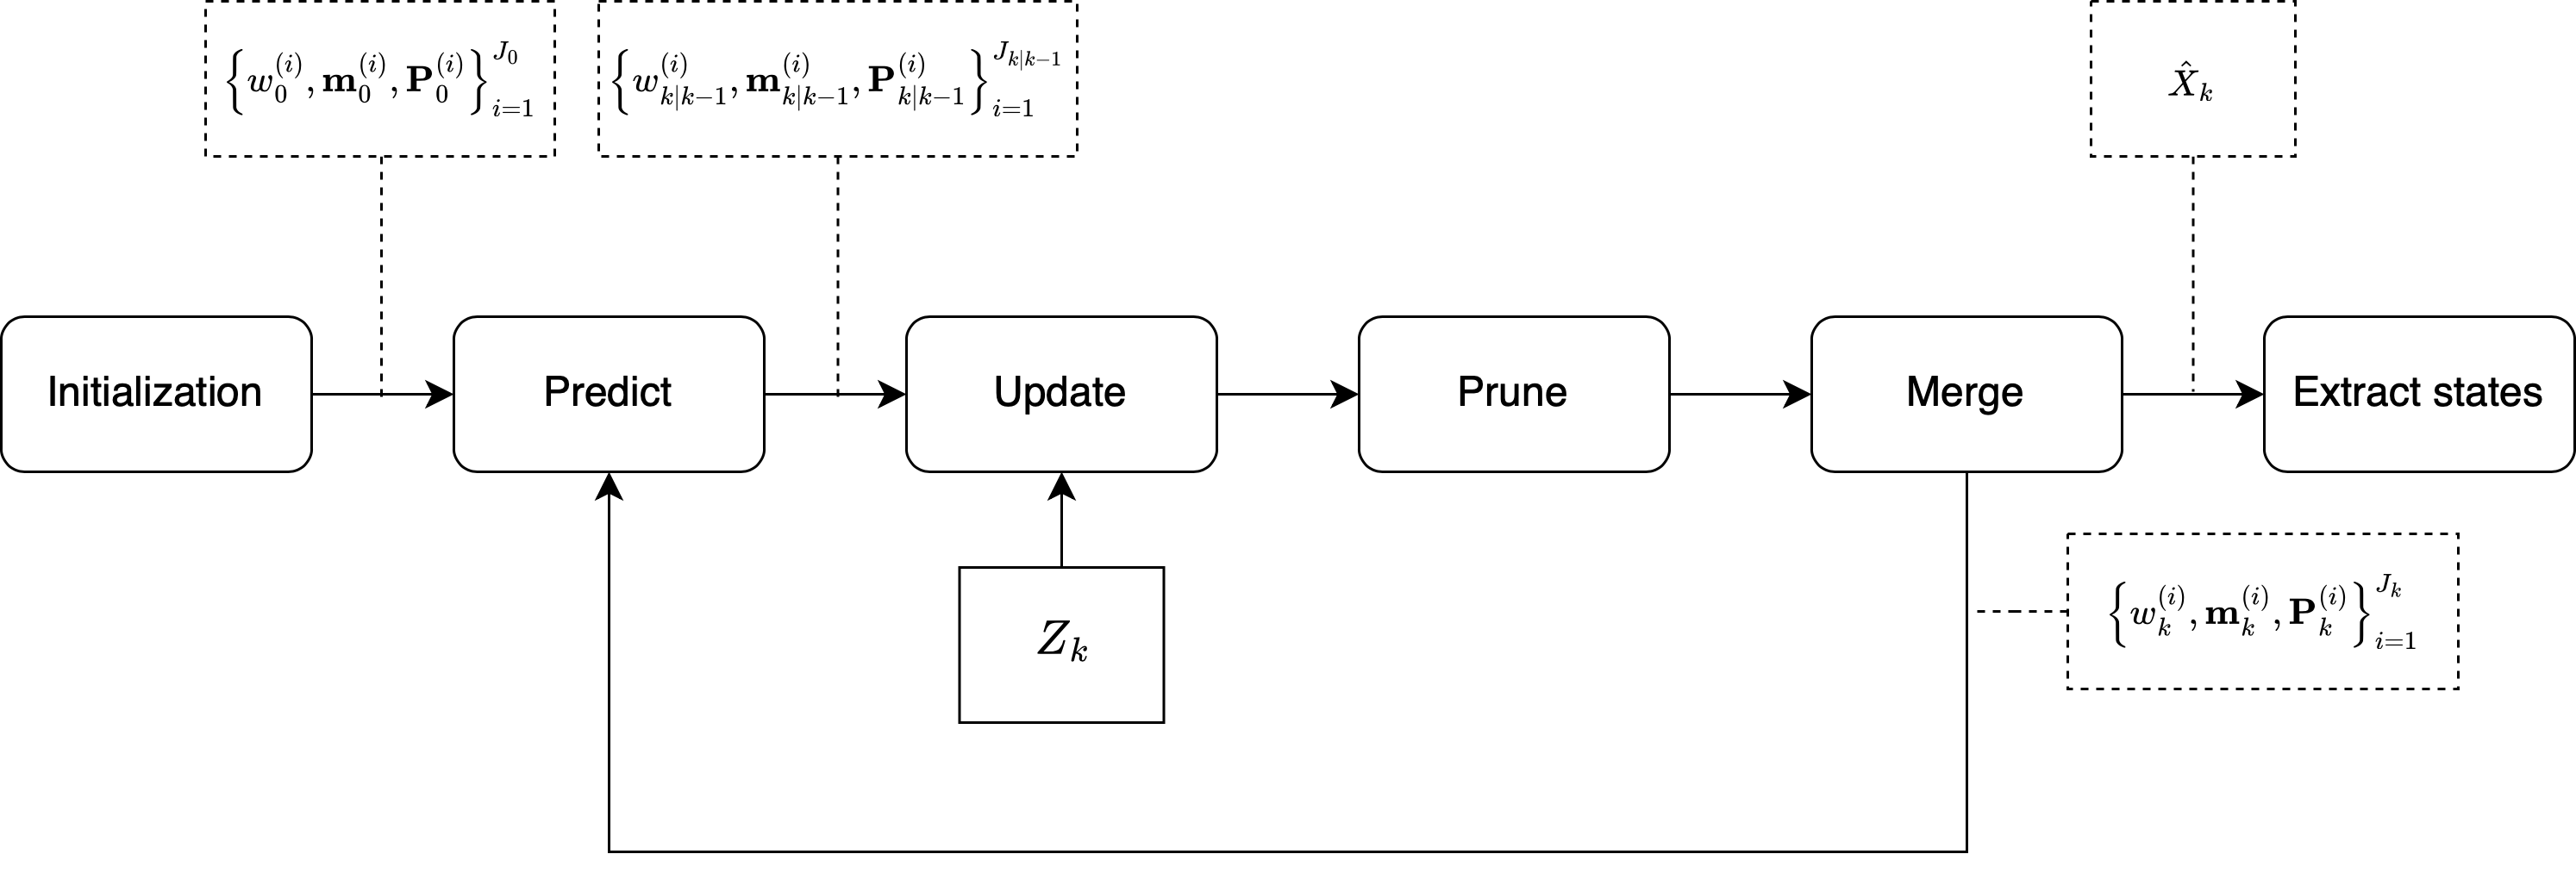
\includegraphics[width=.95\linewidth]{figures/gm-phd-cycle.png}
    \caption[GM-PHD Cycle.]{The visualization of the GM-PHD cycle.}
    \label{fig:gm-phd-cycle}
\end{figure}

            \subsubsection{External information fusion}\label{sec:gm-phd-fusion}
                In many real-world scenarios, one sensor and one source of information may not suffice. Sensors in general have specific technical specifications and limitations. For example, imagine a surveillance system tracking enemy troops. A raw image from a camera working in the visible spectrum may not capture information about people using camouflage, and therefore, tracking such targets with this camera alone becomes intractable. However, if we use additional information from an infrared camera, targets become clearly visible and combined measurements will have a higher signal-to-noise ratio. Techniques involving combining information from different sources are called information fusion. In this section, we will briefly describe the types of information fusion that exist and describe how this information can be used to get more accurate tracking results for the GM-PHD filter.

Information fusion, or information integration, is generally a broad term, mainly because sources of information differ a lot. For instance, \textit{data fusion} is the process of merging data from different data sources and in different formats to create a comprehensive picture of the environment \cite{kleinSensorDataFusion2004}. Data sources may refer to measurements from sensors, data from a database, or human input, while data types may include text, images, audio inputs, or binary data. On the other hand, \textit{decision fusion} refers to collecting decisions from different algorithms that may look at the problem from different perspectives or work with different data inputs, and combining these decisions to create one final decision. Ensembles of different machine learning algorithms, for example, for pattern prediction, are an example of decision fusion \cite{mangaiSurveyDecisionFusion2010}.

In this work, we will refer to another fusion technique called \textit{sensor fusion}. In principle, sensor fusion is a subset of data fusion, which involves collecting data from various sensors and merging it to get a more precise and complete estimate of the environment. The example from the introduction to this section is also an example of sensor fusion. There may be many different types of sensors, including cameras, radars, lidars, sonars, or infrared cameras. Every sensor measures different aspects of the tracked environment, and the combined information describes the surrounding world more precisely.

Regarding Bayesian inference and multi-target tracking, we create estimates of moving objects, and there are many variables that can input uncertainty: the detection rate of the sensor, the quality of the tracking algorithm and its implementation, the environment conditions where the sensor operates, etc. And while the algorithm may be replaced with the one providing better estimates for a specific problem, physical limitations of sensors and the environment cannot be addressed easily. For example, let us take the AN/MPQ-53 radar, which is a part of the Patriot system, a surface-to-air missile system used for air defense deployed in many countries. The exact technical specifications of the radar are far beyond the scope of this work. However, we will give an example of what may cause the radar to fail to detect targets.

The AN/MPQ-53 radar has a 120-degree field of view with a 170 km range \cite{wolffMPQ53Radartutorial}. However, there may be physical limitations of the environment that create blind and clutter zones. For instance, imagine the situation where the radar is deployed on a surface and is targeted to track air objects above the sea. The water may cause spontaneous reflections of the radar rays and cause clutter measurements. Moreover, the curvature of the terrain may create a blind zone so that the radar will not be able to track targets flying at low altitudes. This example is shown graphically in Figure \ref{fig:radar-blind}.

\begin{figure}[ht]
    \centering
    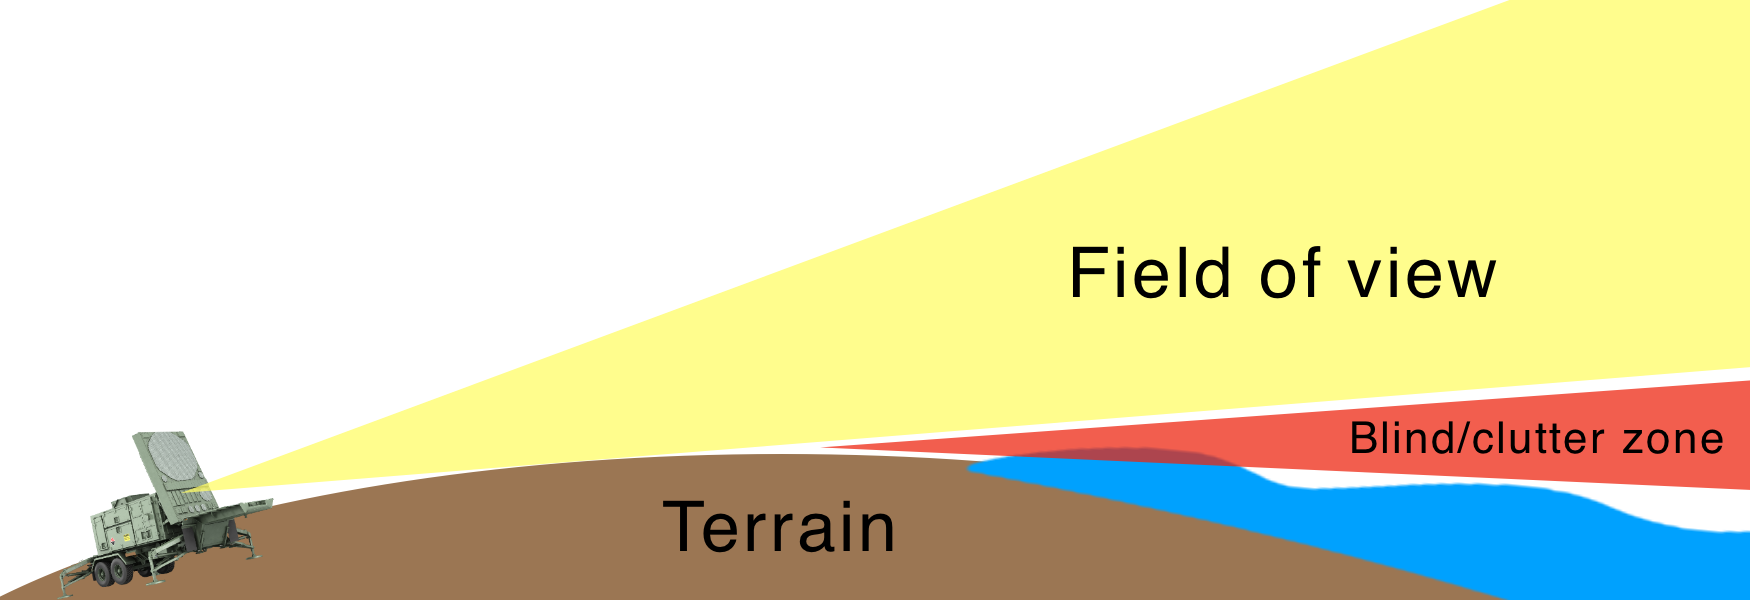
\includegraphics[width=.95\linewidth]{figures/radar-blind.png}
    \caption[Example of a radar blind zone caused by the curvature of the terrain and reflections from water surface.]{An example of the AN/MPQ-53 radar deployed on the surface with curvature and targeted at the sea. The curvature causes the blind zone, and reflections from the water surface may cause clutter measurements.}
    \label{fig:radar-blind}
\end{figure}

This problem may be addressed in several ways, one of which, that is covered in this work, is to use information fusion techniques. For example, we can incorporate additional information from other sensors placed after the curvature that supplements additional data about the blind zone and therefore covers the area that stays invisible to the radar. This source of additional information may be another radar or a different type of sensors, or even a soldier with binoculars. We can then input this additional information to the GM-PHD filter to improve the tracking performance. The example of such mitigation is illustrated in Figure \ref{fig:radar-additional-range}.

\begin{figure}[ht]
    \centering
    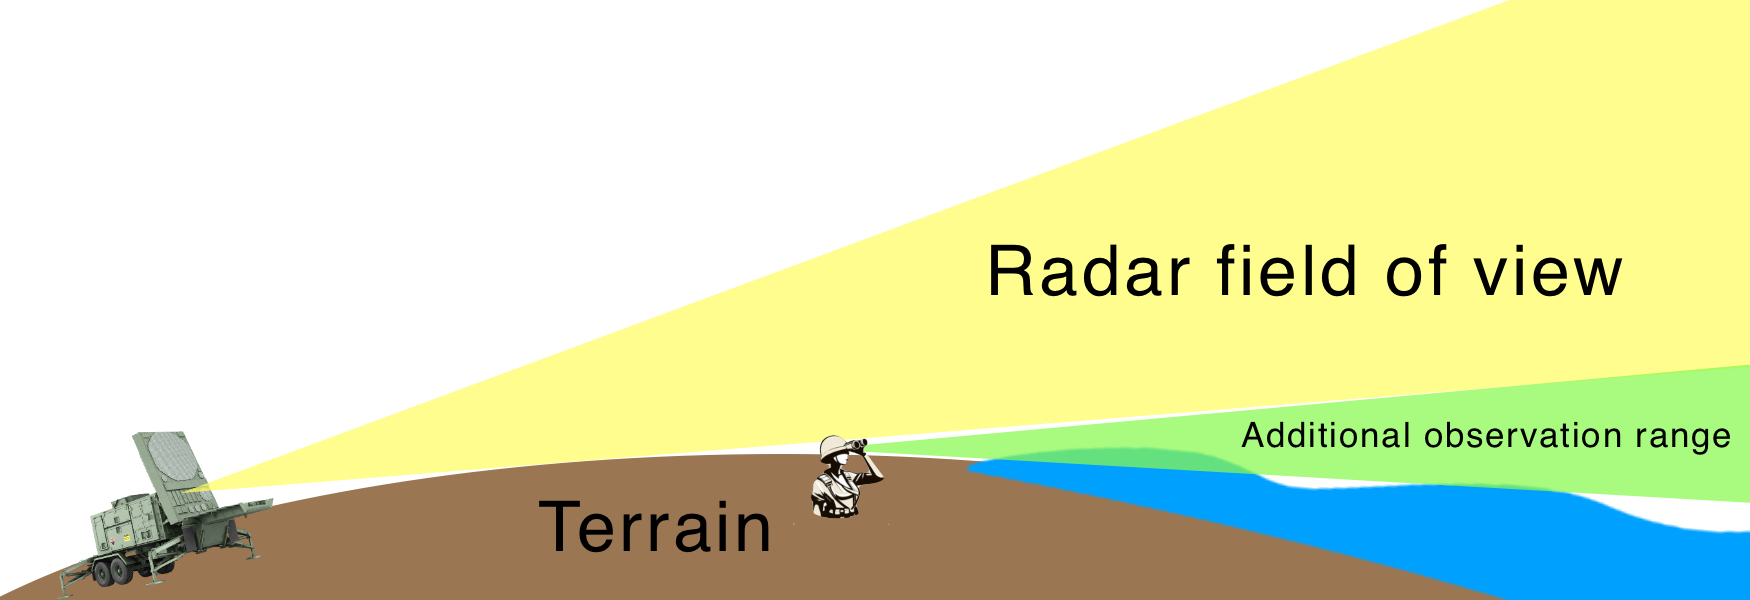
\includegraphics[width=.95\linewidth]{figures/radar-additional-range.png}
    \caption[Example of radar blind zone mitigated with additional observation range from soldier with binoculars.]{An example of the AN/MPQ-53 radar deployed on the surface with curvature and targeted at the sea. After the curvature, there is a soldier with binoculars with the additional observation range that covers the blind zone of the deployed radar.}
    \label{fig:radar-additional-range}
\end{figure}

We now define the imputation of additional data formally. Given that an instance of the GM-PHD filter with the CV model is running and at every time step $k$ it gets measurements from a sensor mixed with clutter in a set $Z_k$. Let there be an additional sensor that operates in the blind zone of the first radar. The second sensor measures position and velocity of targets $\vecat{m}{\psi}$ appearing in the blind zone with the uncertainty given by the covariance matrix $\vecat{P}{\psi}$ and the weight denoting the expected number of targets at this location, denoted $w_{\psi, k}$. Also, every such component is assigned with a unique tag $T_{\psi, k}$. All measurements of the second sensor create a set of additional states at time $k$, denoted $\Psi_{F, k} = \{ w_{\psi, k}^{(i)}, \svecat{m}{\psi}{(i)}, \vecat{P}{\psi}{(i)}, T_{\psi, k}^{(i)} \}_{i=1}^{J_{\psi, k}}$, where $J_{\psi, k}$ denotes the number of additional state estimates. Given that the dynamics of targets is Gaussian-linear, we propose that the intensity function of these additional measurements as $\psi_k(\mathbf{x})$, which is a Gaussian mixture of the following form:

\begin{equation}\label{eq:gm-phd-fusion-fusion-intensity}
    \psi_k(\mathbf{x}) = \sum_{i=1}^{J_{\psi, k}} w_{\psi, k}^{(i)}
        \mathscr{N}\left(\mathbf{x}; \vecat{m}{\psi, k}^{(i)}, \vecat{P}{\psi, k}^{(i)}\right).
\end{equation}

The GM-PHD filter is then modified to include additional information. We include this intensity in the prediction step of the GM-PHD filter, defined in Theorem \ref{theorem:gm-phd-prediction}, that will thus have the following form:

\begin{theorem}[The GM-PHD filter with external information prediction]\label{theorem:gm-phd-fusion-prediction}
    Given that assumptions from Section \ref{sec:gm-phd} apply and the posterior intensity of the previous time step $v_{k-1}(\vecat{x}{k-1} | Z_{1:k-1})$ is a Gaussian mixture of the form:

    \begin{equation}
        v_{k-1}(\vecat{x}{k-1} | Z_{1:k-1}) = \sum_{i=1}^{J_{k-1}}
        \mathscr{N}\left(\vecat{x}{k-1}; \vecat{m}{k-1}^{(i)}, \vecat{P}{k-1}^{(i)}\right),
    \end{equation}

    \noindent where every Gaussian component has a unique tag or label assigned to it, which forms the set of tags:

    \begin{equation}
        T_{k-1} = \{ T_{k-1}^{(1)}, \ldots, T_{k-1}^{(J_{k-1})} \}.
    \end{equation}

    \noindent Also, let additional state estimates from other sensors have the form $\Psi_{F, k} = \{ w_{\psi, k}^{(i)}, \svecat{m}{\psi}{(i)}, \svecat{P}{\psi}{(i)}, \allowbreak T_{\psi, k}^{(i)} \}_{i=1}^{J_{\psi, k}}$ and the fusion intensity is given by Equation \ref{eq:gm-phd-fusion-fusion-intensity}. Then the predicted intensity at time $k$ is also a Gaussian mixture, defined as:

    \begin{equation}
        v_{k|k-1}(\vecat{x}{k} | Z_{1:k-1}) = \gamma_k(\vecat{x}{k}) + \psi_k(\vecat{x}{k}) + v_{S, k|k-1}(\vecat{x}{k}),
    \end{equation}

    \noindent where $\gamma_k(\vecat{x}{k})$ is given in Equation \ref{eq:gm-phd-birth-gm} and $v_{S, k|k-1}(\vecat{x}{k})$ is the PHD function of survived targets given in Theorem \ref{theorem:gm-phd-prediction}. The set of tags after the prediction step forms the union of the set of tags from the previous time step with the set of unique tags of components spontaneously born at time $k$ and tags from Gaussian terms from another sensor:

    \begin{equation}
        T_{k|k-1} = T_{k-1} \cup \{ T_{\gamma_k}^{(1)}, \ldots, T_{\gamma_k}^{(J_{\gamma_k})} \}
        \cup \{ T_{\psi}^{(1)}, \ldots, T_{\psi}^{(J_{\psi})} \}.
    \end{equation}
\end{theorem}

All other steps of the GM-PHD filter remain the same. The final algorithm of the GM-PHD filter with external information fusion is given in Algorithm \ref{alg:gm-phd}.

\begin{algorithm}
\caption{GM-PHD filter with additional information fusion}\label{alg:gm-phd}
\begin{algorithmic}[1]
    \Require Truncation threshold $\tau$
    \Require Merge threshold $U$
    \Require Maximum number of components $J_\mathrm{max}$
    \Require Initial Gaussian terms $v_0 = \{ w_{0}^{(i)}, \vecat{m}{0}^{(i)}, \vecat{P}{0}^{(i)}, T_0^{(i)}\}_{i=1}^{J_0}$

    \item[]
    \Procedure{GM-PHD-Fusion}{$Z_k, \Psi_k, v_{k-1} = \{ w_{k-1}^{(i)}, \vecat{m}{k-1}^{(i)}, \vecat{P}{k-1}^{(i)}, T_{k-1}^{(i)}\}_{i=1}^{J_{k-1}}$}\label{alg:gm-phd:step}
        \State $v_{k|k-1} \gets \Call{Predict-Fuse}{\Psi_k, v_{k-1}}$
        \State $v_{k} \gets \Call{Update}{Z_k, v_{k|k-1}}$ \Comment{Defined in Algorithm \ref{alg:gm-phd:update}}
        \State $\bar{v}_k \gets \Call{Prune}{\tau, v_{k}}$ \Comment{Defined in Algorithm \ref{alg:gm-phd:prune}}
        \State $\tilde{v}_k \gets \Call{Merge}{U, \bar{v}_k}$ \Comment{Defined in Algorithm \ref{alg:gm-phd:merge}}
        \State $\hat{X} \gets \Call{StateExtract}{\tilde{v}_k}$ \Comment{Defined in Algorithm \ref{alg:gm-phd:extract-states}}
        \State \Return $\hat{X}$
    \EndProcedure
    
    \item[]
    \Procedure{Predict-Fuse}{$\Psi_k, \{ w_{k-1}^{(i)}, \vecat{m}{k-1}^{(i)}, \vecat{P}{k-1}^{(i)}, T_{k-1}^{(i)}\}_{i=1}^{J_{k-1}}$}\label{alg:gm-phd:predict-fuse}
        \State $j \gets 0$
        \For{$i \gets 1, \ldots, J_{\gamma, k}$} \Comment{Create spontaneous birth components}
            \State $i \gets i + 1$
            \State $w_{k|k-1}^{(j)} \gets w_{\gamma, k}^{(i)}$
            \State $\vecat{m}{k|k-1}^{(j)} \gets \vecat{m}{\gamma, k}^{(i)}$
            \State $\vecat{P}{k|k-1}^{(j)} \gets \vecat{P}{\gamma, k}^{(i)}$
            \State $T_{k|k-1}^{(j)} \gets T_{\gamma, k}^{(i)}$
        \EndFor

        \For{$i \gets 1, \ldots, J_{\psi, k}$} \Comment{Fuse external information}
            \State $i \gets i + 1$
            \State $w_{k|k-1}^{(j)} \gets w_{\psi, k}^{(i)}$
            \State $\vecat{m}{k|k-1}^{(j)} \gets \vecat{m}{\psi, k}^{(i)}$
            \State $\vecat{P}{k|k-1}^{(j)} \gets \vecat{P}{\psi, k}^{(i)}$
            \State $T_{k|k-1}^{(j)} \gets T_{\psi, k}^{(i)}$
        \EndFor

        \For{$i \gets 1, \ldots, J_{k-1}$} \Comment{Prediction for existing targets}
            \State $i \gets i + 1$
            \State $w_{k|k-1}^{(j)} \gets P_{S,k} w_{k-1}^{(i)}$
            \State $T_{k|k-1}^{(j)} \gets T_{k-1}^{(i)}$
            \State $\vecat{m}{S,k|k-1}^{(i)} \gets \vecat{F}{k-1}\vecat{m}{k-1}^{(i)}$
            \State $\vecat{P}{S,k|k-1}^{(i)} \gets \vecat{F}{k-1} \vecat{P}{k-1}^{(i)} \vecat{F}{k-1}^\intercal + \vecat{Q}{k-1}$
        \EndFor

        \State $J_{k|k-1} \gets j$
        
        \State \Return $\{ w_{k|k-1}^{(i)}, \vecat{m}{k|k-1}^{(i)}, \vecat{P}{k|k-1}^{(i)}, T_{k|k-1}^{(i)}\}_{i=1}^{J_{k|k-1}}$
    \EndProcedure

\end{algorithmic}
\end{algorithm}

In this chapter, we introduced the fundamentals of multi-object tracking and discussed ways how we can track multiple targets using measurements from a sensor in clutter. Subsequently, we described the PHD filter, which utilizes the Final Set Statistics to propagate the posterior intensity function of the multi-target probability distribution. Furthermore, we introduced the GM-PHD filter, a closed-form solution of the PHD filter for Gaussian-linear dynamics of moving objects. Lastly, we extended the GM-PHD filter with fusion of external information, which enhanced the tracking performance for those cases where one sensor may fail to detect targets due to the effects of physical limitations of the sensor or environment. In the next chapter, we will describe the implementation of the GM-PHD filter and its performance on different testing cases and metrics.


%%%%%%%%%%%%%%%%%%%%%%%%%%%%%%%%%%%%%%%%%%
% Implementation and testing
%%%%%%%%%%%%%%%%%%%%%%%%%%%%%%%%%%%%%%%%%%
\chapter{Implementation and tests}\label{ch:implementation}
    This chapter presents the methodology we used to test the performance of the GM-PHD filter. Firstly, we introduce two metrics that are appropriate for use in measuring the performance of a multi-target tracking algorithm. Secondly, we describe in detail several test scenarios on which the testing was conducted. Finally, we explain the ranges of different initial settings that were tested and describe the implementation of the GM-PHD filter.

    \section{Metrics}\label{sec:metrics}
        For evaluating the performance of the GM-PHD filter, we used two metrics proposed in \cite{voGaussianMixtureProbability2006}. The first metric is called the Circular Position Error Probability (CPEP). It measures the probability that the estimated position of a target falls in a circular region with a given radius around the true position. This metric has its roots in the military area, where the weapons system precision is measured with the probability of hitting targets in a certain ellipse with a given mean \cite{nelsonUseCircularError}. While linear metrics like a simple Euclidean distance would measure the accuracy, the CPEP metrics measures precision of the tracking algorithm. In formal language, this metric is defined as:

\begin{equation}
    \operatorname{CPEP}_k (r) = \frac{1}{|X_k|} \sum_{\mathbf{x} \in X_k} \rho_k(\mathbf{x}, r),
\end{equation}

\noindent where $r$ is the radius of the circluar area, and $\rho_k(\mathbf{x}, r)$ is defined as:

\begin{equation}
     \rho_k(\mathbf{x}, r) = \Pr{\| \mathbf{H}_k \mathbf{\hat{x}} - \mathbf{H}_k \mathbf{x}\|_2 > r, \forall \mathbf{\hat{x}} \in \Hat{X}_k}.
\end{equation}

\noindent Here, $\hat{X}_k$ refers to the set of estimates generated by the tracking algorithm at time step $k$, $\mathbf{H}_k$ is the single-target measurement model, and $\| \cdot \|_2$ is the Euclidean norm of a vector.

The second measure of tracking error is the expected absolute error on the number of targets. In simple words, this metric gives the average difference between the predicted and true number of targets. Mathematically, it is defined as:

\begin{equation}
    E\left[ \left||\hat{X}_k| - |X_k|\right| \right].
\end{equation}

Generally, these two metrics measure the total uncertainty of a multi-target tracking filter given be a random finite set -- both the number of targets in the set and the precision of the estimates. We evaluate these metrics for all tracking scenarios to show the influence of a parameter change or the presence of fusion techniques on the filter performance.

    \section{Test scenarios}\label{sec:test-scenarios}
        We evaluate the algorithm's performance in four different test scenarios using multiple parameter values. To facilitate reference to these scenarios later in the report, we denote them as \textbf{(C1)}--\textbf{(C4)}. The following subsections provide a detailed description of each test case. Here, we describe the complete setup common to all scenarios.

All test cases use the Gaussian-linear Constant Velocity motion and measurement models described in Section \ref{sec:cv-model}. Targets are assumed to move in 2D Euclidean space, where distance is measured in meters and time in seconds. Additionally, we assume that the sampling period is constant and set to $1 s$. The process noise $q$ is set to $5 m/s^2$ for every target and every test case. Consequently, the single-target state vector $\vecat{x}{k}$, the single-target state transition matrix $\mathbf{F}$, and the process noise matrix $\mathbf{Q}$ have the following form:

\begin{equation}
    \vecat{x}{k} =
    \begin{bmatrix}
        x_{k} \\ 
        y_{k} \\ 
        v_{x,k} \\ 
        v_{y,k}
    \end{bmatrix};
    \quad
    \mathbf{F} =
    \begin{bmatrix}
       1 & 0 & 1 & 0 \\
       0 & 1 & 0 & 1 \\
       0 & 0 & 1 & 0 \\
       0 & 0 & 0 & 1 
    \end{bmatrix};
    \quad
    \mathbf{Q} = \begin{bmatrix}
        \frac{25}{3}    & 0             & \frac{25}{2}      & 0  \\
        0               & \frac{25}{3}  & 0                 & \frac{25}{2} \\
        \frac{25}{2}    & 0             & 25                & 0 \\
        0               & \frac{25}{2}  & 0                 & 25
    \end{bmatrix}.
\end{equation}

Moreover, we set the standard deviation of the measurement noise to a constant value for all test cases, $r = 10 m$. The measurement matrix $\mathbf{H}$ and the measurement noise matrix $\mathbf{R}$ are defined as:

\begin{equation}
    H =
    \begin{bmatrix}
        1 & 0 &0 & 0 \\
        0 & 1 &0 & 0
    \end{bmatrix};
    \quad
    R = \begin{bmatrix}
        100 & 0   \\
        0   & 100
    \end{bmatrix}.
\end{equation}

The sensor's field of view is a 2D square with an area of $V = 4 \times 10^6 m^2$, with boundaries delimited by $[-1000, 1000] \times [-1000, 1000]$ meters. This rectangular region corresponds to the surveillance area where the sensor is deployed. The sensor is assumed to be perfect with infinite resolution.

The initial detection and survival probabilities are set to $P_{D,k} = 0.98$ and $P_{S,k} = 0.99$, respectively. We will see the metrics for different values of these parameters in the next chapter.

The birth process is initialized as a Gaussian mixture with two components, where each component represents the location where new targets are expected to be born and its weight denotes the likelihood of a real target being present in the area. The specific relationships for each test case differ and will be presented in the following subsections.

The noise process is modeled using a Poisson random finite set, and the clutter measurements are Poisson distributed in time and uniformly distributed in space. The clutter intensity is denoted by a normalized intensity over the surveillance region, the clutter spatial intensity $\lambda_c$, and is set to a constant $\lambda_c = 12.5 \times 10^{-6} m^{-2}$. With the surveillance area equal to $V = 4 \times 10^6 m^2$, this Poisson process generates on average 50 clutter measurements at each time step. In later sections, we will evaluate the impact of changing the spatial clutter intensity, represented by the parameter $\lambda_c$, on the performance of the GM-PHD filter by testing it for different values of $\lambda_c$. This clutter process is described by the following equation:

\begin{equation}
\kappa_k(\mathbf{z}) = \lambda_c V u(\mathbf{z}),
\end{equation}

\noindent where $u(\mathbf{z})$ represents the bivariate uniform distribution over the surveillance area $[x_0, x_1] \times [y_0, y_1]$, given by:

\begin{equation}
    u(\mathbf{z}) = \begin{cases}
        \frac{1}{(x_1 - x_0)(y_1 - y_0)}, & \mathbf{z} \in [x_0, x_1] \times [y_0, y_1], \\
        0, & \text{otherwise}.
    \end{cases}
\end{equation}

The truncation threshold for the pruning step of the GM-PHD filter is set to $\tau = 10^{-5}$, and the merging threshold is set to $U = 4$. The impact of changing these parameters on the filter's performance will be discussed. The maximum number of components is fixed at $J_{\mathrm{max}} = 1000$, intentionally set higher than the value proposed in \cite{voGaussianMixtureProbability2006} to evaluate different parameter settings with more precision, particularly in scenarios with a higher number of targets.

In the following subsections, we will provide a detailed description of the dynamics of targets for each test case. We will then evaluate the GM-PHD filter's performance for each scenario and discuss the results.

        \subsection{Two objects with crossing paths (C1)}\label{sec:c1-scenario}
            This test case is fully identical to the one given in \cite{voGaussianMixtureProbability2006} and demonstrates the accuracy of the implementation by showing that the results obtained by the authors of the original paper are reproducible.

In this scenario, two objects are born at the same time at $k=1$ and follow independent linear paths. The initial state vectors of these objects are the following:

\begin{equation}
    \svecat{x}{1}{(1)} = \begin{bmatrix}
        250.0 \\
        250.0 \\
        2.5 \\
        -12.0
    \end{bmatrix},
    \qquad
    \svecat{x}{1}{(2)} = \begin{bmatrix}
        -250.0 \\
        -250.0 \\
        12 \\
        -2.5
    \end{bmatrix}.
\end{equation}

At a certain moment, their tracks cross. Both objects disappear at time $k=100$. Therefore, the number of objects remains constant throughout the simulation, with two objects present at all times. The paths of both objects are shown in Figure \ref{fig:c1-scenario}. The arrows show the direction of movement, and the position of the arrowhead denotes the position of the object's death. The circles on the other side of the line illustrate the location of the target birth.

\begin{figure*}
    \centering
    \begin{subfigure}[]{0.48\linewidth}
        \centering
        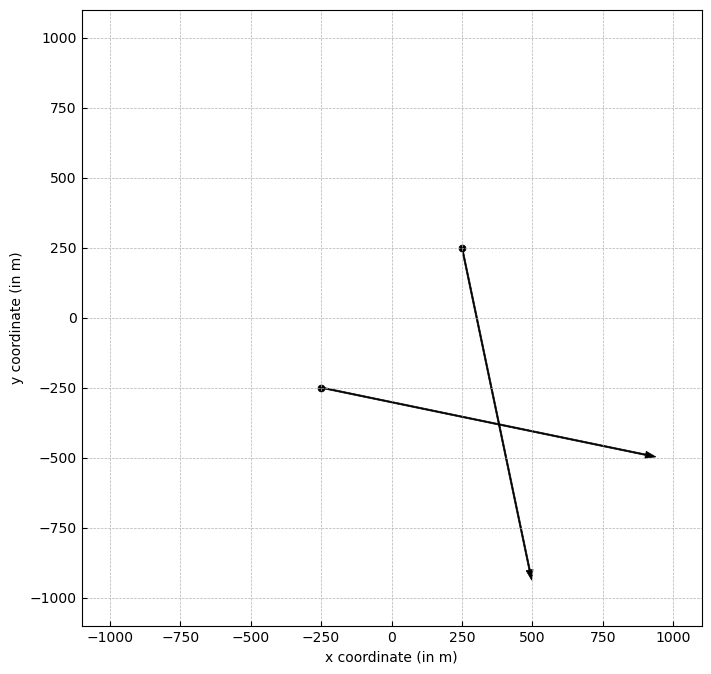
\includegraphics[width=\linewidth]{figures/c1-tracks.png}
    \end{subfigure}
    \hfill
    \begin{subfigure}[]{0.48\linewidth}
        \centering
        \begin{subfigure}[t]{\linewidth}
            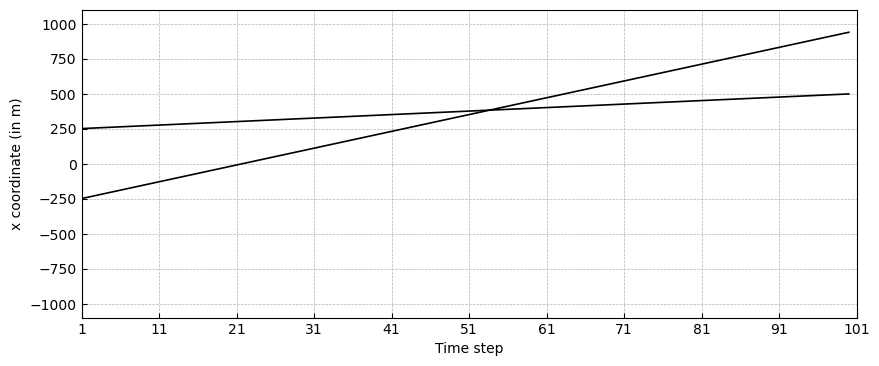
\includegraphics[width=\linewidth]{figures/c1-coord-x.png}
        \end{subfigure}
        \vfill\par
        \begin{subfigure}[b]{\linewidth}
            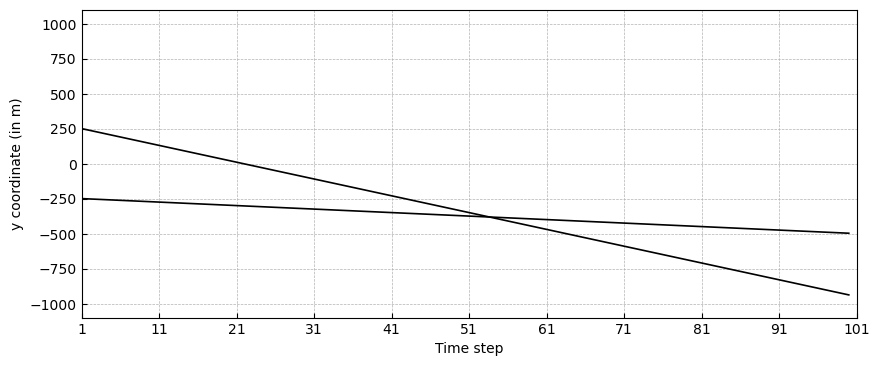
\includegraphics[width=\linewidth]{figures/c1-coord-y.png}
        \end{subfigure}
    \end{subfigure}
  \caption[True tracks of objects in the (C1) scenario.]{The (C1) scenario. On the left figure, we see the tracks of two objects in the 2D space, locations of their births (black circles) and deaths (arrow heads). On the right figure, we see how each coordinate of the tracks of both objects changes over time. We can see that the tracks of two objects intersect at time $k=53$.}
  \label{fig:c1-scenario}
\end{figure*}

Finally, the initial Gaussian mixture of the birth intensity in this scenario is given by:

\begin{equation}
    \gamma_k(\mathbf{x}) = 0.1 \mathscr{N}\left( \mathbf{x}; \svecat{m}{\gamma}{(1)}, \vecat{P}{\gamma} \right)
        + 0.1 \mathscr{N}\left( \mathbf{x}; \svecat{m}{\gamma}{(2)}, \vecat{P}{\gamma} \right),
\end{equation}

\noindent where:

\begin{equation}
    \svecat{m}{\gamma}{(1)} = \begin{bmatrix}
        250 \\
        250 \\
        0 \\
        0 \\
    \end{bmatrix},
    \qquad
    \svecat{m}{\gamma}{(2)} = \begin{bmatrix}
        -250 \\
        -250 \\
        0 \\
        0 \\
    \end{bmatrix},
    \qquad
    \vecat{P}{\gamma} = \begin{bmatrix}
        100 & 0     & 0     & 0     \\
        0   & 100   & 0     & 0     \\
        0   & 0     & 25    & 0     \\
        0   & 0     & 0     & 25    \\
    \end{bmatrix}.
\end{equation}

        \subsection{Objects are born and die at different times (C2)}\label{sec:c2-scenario}
            This test case represents a scenario in which different objects are born at different times and move in various directions. It demonstrates how well the filter performs on tracking multiple objects when the number of true targets $X_k$ changes over time.

The birth intensity consists of two Gaussian terms, as in the (C1) case, each with a weight of $0.1$, and is expressed as follows:

\begin{equation}\label{eq:c2-birth}
    \gamma_k(\mathbf{x}) = 0.1 \mathscr{N}\left( \mathbf{x}; \svecat{m}{\gamma}{(1)}, \vecat{P}{\gamma} \right)
        + 0.1 \mathscr{N}\left( \mathbf{x}; \svecat{m}{\gamma}{(2)}, \vecat{P}{\gamma} \right),
\end{equation}

\noindent where:

\begin{equation}\label{eq:c2-birth-means}
    \svecat{m}{\gamma}{(1)} = \begin{bmatrix}
        -1000 \\
        750 \\
        0 \\
        0 \\
    \end{bmatrix},
    \qquad
    \svecat{m}{\gamma}{(2)} = \begin{bmatrix}
        1000 \\
        -750 \\
        0 \\
        0 \\
    \end{bmatrix},
    \qquad
    \vecat{P}{\gamma} = \begin{bmatrix}
        100 & 0     & 0     & 0     \\
        0   & 100   & 0     & 0     \\
        0   & 0     & 30    & 0     \\
        0   & 0     & 0     & 30    \\
    \end{bmatrix}.
\end{equation}

In total, there are six different tracks, with a maximum of five targets present at a time and a minimum of one target at a time step. Objects are born every $10$ time steps, and each has a lifespan of $50$ time steps. The paths of the six targets are depicted in Figure \ref{fig:c2-scenario}. The state vectors of the six targets are as follows:

\begin{alignat}{3}\label{eq:c2-init-states}
    \svecat{x}{0}{(1)} &= \begin{bmatrix}
        -1000.0 \\
        750.0 \\
        25.0 \\
        0.0
    \end{bmatrix},
    &\qquad
    \svecat{x}{10}{(2)} &= \begin{bmatrix}
        1000.0 \\
        -750.0 \\
        -25.0 \\
        0.0
    \end{bmatrix},
    &\qquad
    \svecat{x}{20}{(3)} &= \begin{bmatrix}
        -1000.0 \\
        750.0 \\
        17.68 \\
        -17.68
    \end{bmatrix},
    \nonumber \\
    \svecat{x}{30}{(4)} &= \begin{bmatrix}
        1000.0 \\
        -750.0 \\
        -17.68 \\
        17.68
    \end{bmatrix},
    &\qquad
    \svecat{x}{40}{(5)} &= \begin{bmatrix}
        -1000.0 \\
        750.0 \\
        0.0 \\
        -25.0
    \end{bmatrix},
    &\qquad
    \svecat{x}{50}{(6)} &= \begin{bmatrix}
        1000.0 \\
        -750.0 \\
        0.0 \\
        25.0
    \end{bmatrix}.
\end{alignat}

\begin{figure*}
    \centering
    \begin{subfigure}[]{0.48\linewidth}
        \centering
        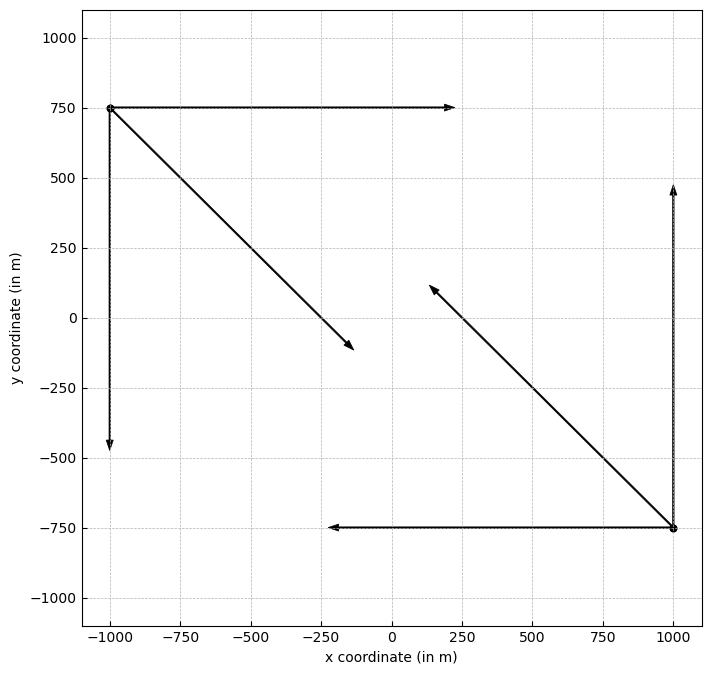
\includegraphics[width=\linewidth]{figures/c2-tracks.png}
    \end{subfigure}
    \hfill
    \begin{subfigure}[]{0.48\linewidth}
        \centering
        \begin{subfigure}[t]{\linewidth}
            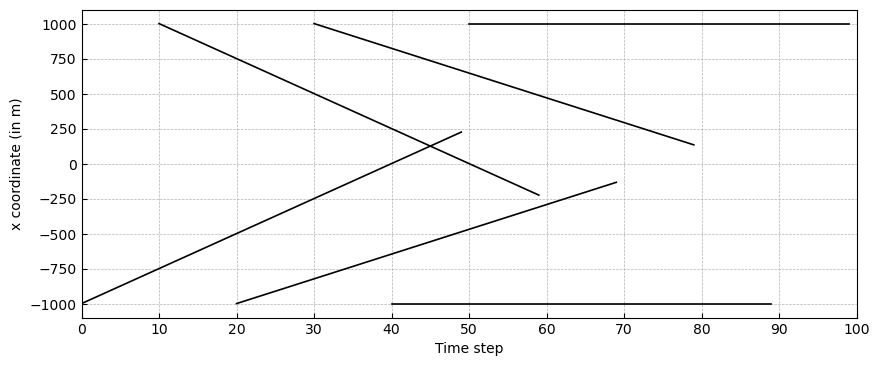
\includegraphics[width=\linewidth]{figures/c2-coord-x.png}
        \end{subfigure}
        \vfill\par
        \begin{subfigure}[b]{\linewidth}
            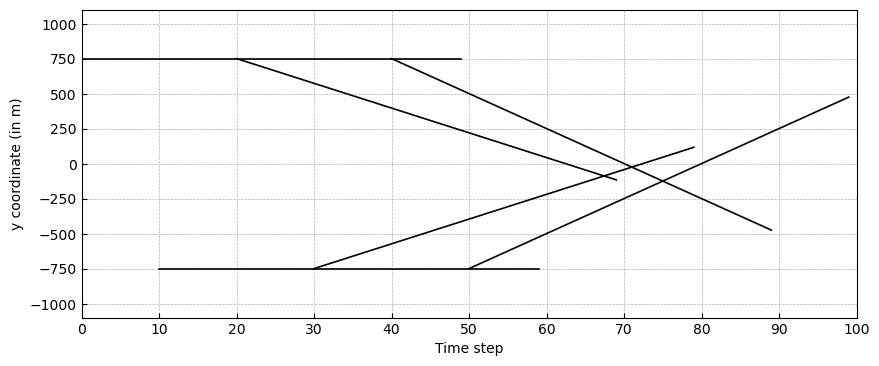
\includegraphics[width=\linewidth]{figures/c2-coord-y.png}
        \end{subfigure}
    \end{subfigure}
  \caption[True tracks of objects in the (C2) scenario.]{The (C2) scenario. In the left figure, we can see the tracks of multiple objects in the 2D space, their locations of birth (black circles) and death (arrow heads). The right figure shows how the coordinates of each object track change over time and the variation in the number of objects present in the scene.}
  \label{fig:c2-scenario}
\end{figure*}

        \subsection{Unexpected objects with no fusion (C3)}\label{sec:c3-scenario}
            The third scenario is based on the second one, (C2), and it tests the appearance of two additional components on two unexpected locations. The birth intensity is defined by the same relation as in Equations \ref{eq:c2-birth} and \ref{eq:c2-birth-means}. The initial states of objects, including the time of birth is also the same and given by Equation \ref{eq:c2-init-states}. However, there are also two additional objects entering the scene at time $k=20$ and $k=60$. Their initial state vector are given by:

\begin{equation}\label{eq:c3-additional-states}
    \svecat{x}{20}{(7)} = \begin{bmatrix}
        -1000.0 \\
        -1000.0 \\
        20.0 \\
        20.0
    \end{bmatrix},
    \qquad
    \svecat{x}{60}{(8)} = \begin{bmatrix}
        1000.0 \\
        1000.0 \\
        -20.0 \\
        -20.0
    \end{bmatrix}.
\end{equation}

The lifespan of these objects is $40$ time steps of each. The whole picture of tracks in the scene is depicted in Figure 

\begin{figure*}
    \centering
    \begin{subfigure}[]{0.48\linewidth}
        \centering
        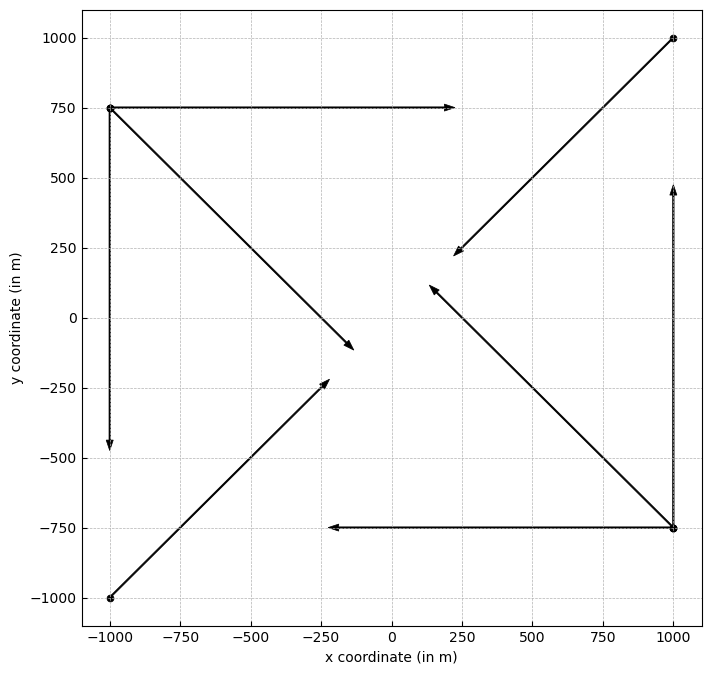
\includegraphics[width=\linewidth]{figures/c3-tracks.png}
    \end{subfigure}
    \hfill
    \begin{subfigure}[]{0.48\linewidth}
        \centering
        \begin{subfigure}[t]{\linewidth}
            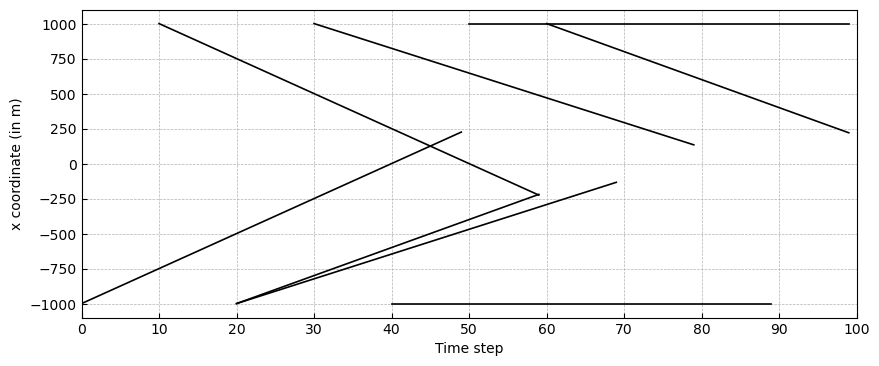
\includegraphics[width=\linewidth]{figures/c3-coord-x.png}
        \end{subfigure}
        \vfill\par
        \begin{subfigure}[b]{\linewidth}
            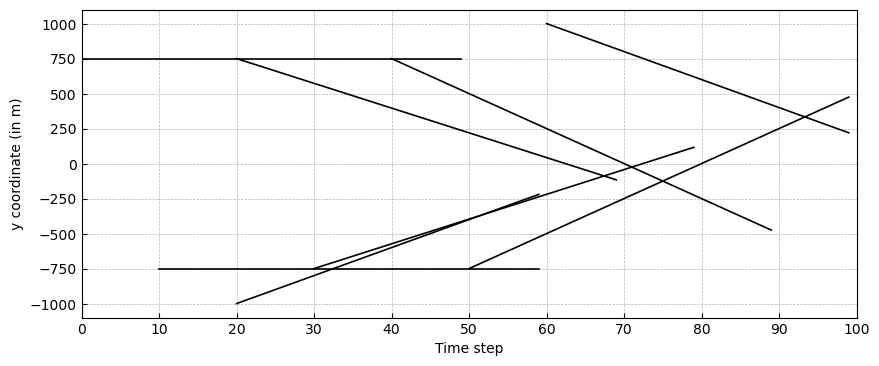
\includegraphics[width=\linewidth]{figures/c3-coord-y.png}
        \end{subfigure}
    \end{subfigure}
  \caption[True tracks of objects in the (C3) scenario.]{The (C3) scenario. On the left figure, we can see the tracks of multiple objects in the 2D space, their locations of birth (black circles) and death (arrow heads). In comparison to the (C2) case, two additional objects appear on two additional positions. The right figure shows how the coordinates of each object's track change over time.}
  \label{fig:c3-scenario}
\end{figure*}

For instance, this scenario may occur in cases when a sensor has a blind zone, and the objects appear in the field of view too late. We will later show that without imputation of external information, the GM-PHD filter is unable to capture the dynamics of these objects.

        \subsection{Unexpected objects with external information fusion (C4)}\label{sec:c4-scenario}
            The last test scenario is identical to the previous one, (C3), with the addition of two fused components. The example provided in Section \ref{sec:gm-phd-fusion} suggests that the additional information may be provided by another sensor or, for instance, by a soldier. The filter is then able to capture objects that remain invisible due to its physical limitations or the environmental conditions.

The birth intensity is given by Equations \ref{eq:c2-birth} and \ref{eq:c2-birth-means}. Initial states of moving targets are defined by Equations \ref{eq:c2-init-states} and \ref{eq:c3-additional-states}, and tracks of moving targets are visually demonstrated in Figure \ref{fig:c3-scenario}. However, in this test case, we additionally create fusion sets at times $k=20$ and $k=60$ with one element. At every other time step, the fusion set remains empty. Recall that the fusion intensity $\psi_k$ is given by Equation \ref{eq:gm-phd-fusion-fusion-intensity}. The set $\Psi_{F,k}$ in our scenario is defined as follows:

\begin{equation}
    \Psi_{F, k} = \begin{cases}
        \left\{ ( w_{20}^{(1)}, \svecat{m}{\psi, 20}{(1)}, \svecat{P}{\psi, 20}{(1)}, T_{\psi, 20} )\right\} & \text{if } k = 20, \\
        \left\{ ( w_{60}^{(2)}, \svecat{m}{\psi, 60}{(2)}, \svecat{P}{\psi, 60}{(2)}, T_{\psi, 60} )\right\} & \text{if } k = 60, \\
        \emptyset & \text{otherwise},
    \end{cases}
\end{equation}

\noindent where: 

\begin{alignat}{3}
    w_{20}^{(1)}
    &= 0.6,
    &\qquad
    \svecat{m}{\psi, 20}{(1)}
    &= \begin{bmatrix}
        -1050 \\
        -1050 \\
        25 \\
        25
    \end{bmatrix},
    &\qquad
    \svecat{P}{\psi, 20}{(1)}
    &= \begin{bmatrix}
        100 & 0 & 0 & 0 \\
        0 & 100 & 0 & 0 \\
        0 & 0 & 100 & 0 \\
        0 & 0 & 0 & 100
    \end{bmatrix}, \\
    w_{60}^{(2)}
    &= 0.7,
    &\qquad
    \svecat{m}{\psi, 60}{(2)}
    &= \begin{bmatrix}
        1020 \\
        1020 \\
        -22 \\
        -22
    \end{bmatrix},
    &\qquad
    \svecat{P}{\psi, 60}{(3)}
    &= \begin{bmatrix}
        40 & 0 & 0 & 0 \\
        0 & 40 & 0 & 0 \\
        0 & 0 & 5 & 0 \\
        0 & 0 & 0 & 5
    \end{bmatrix}.
\end{alignat}

\noindent and $T_{\psi, 20}$ and $T_{\psi, 20}$ are some unique tags for new Gaussian components.

We assume that there are two sensors, each measuring at two different locations. The first sensor generates estimates with larger uncertainty; therefore, the covariance matrix has higher values, and the weight, the measure of uncertainty of the sensor, is lower. The second sensor, which inputs information at time $k=60$, has better precision, and the estimate of the position of the second object and its speed is more precise, thus having a higher weight value.

    \section{Parameters testing and methodology}\label{sec:parameters-tests}
        Each test scenario \textbf{(C1)}--\textbf{(C4)} has default settings as defined in Section \ref{sec:test-scenarios}. However, to obtain a complete picture of how the GM-PHD filter behaves in different situations, we also evaluate each test case with various combinations of filter settings. This testing is performed by fixing the default values of every parameter and iterating through different values of one parameter at a time. The list of tested settings includes:

\begin{itemize}
    \item Clutter spatial density $\lambda_c \in [0, 1.25, 2.5, 3.75, 5, 6.25, 7.5, 8.75, 10, 11.25, 12.5] \times 10^{-6}$
    \item Detection probability $P_{D,k} \int [0.7, 0.75, 0.8, 0.85, 0.9, 0.95, 1.0]$
    \item Survival probability $P_{S,k} \int [0.7, 0.75, 0.8, 0.85, 0.9, 0.95, 1.0]$
    \item Truncation threshold $\tau \int [10^{-6}, 10^{-5}, 10^{-4}, 10^{-3}]$
    \item Merge threshold $U \int [4, 10, 20, 50]$
\end{itemize}

The GM-PHD filter with additional information fusion was implemented using Python 3.10 and the following libraries:

\begin{itemize}
    \item NumPy v1.23.5 for mathematical operations and efficient matrix multiplication,
    \item SciPy v1.10.0 for a convenient and reliable sampling from multivariate distributions,
    \item Matplotlib v3.7.0 for plot generation and visualization.
\end{itemize}

Additionally, for numerical stability of calculation of covariance matrices, so that they remain symmetrical and positive definite, a small trick is applied:

\begin{equation}
    \mathbf{P} = 0.5 * (\mathbf{P} + \mathbf{P}^\intercal).
\end{equation}

For each testing scenario and every combination of default settings and changed parameters, a testing case is created. Each testing case is evaluated using $100$ Monte Carlo input data samples, which are randomly generated measurements, clutter, and misdetections. The filter is run on each sample separately, resulting in $100$ filter runs per testing case. In total, we conducted $13,200$ runs of the GM-PHD filter. The testing was performed using a MacBook Pro model A2141 with a 2.6 GHz 6-Core Intel Core i7 CPU and 16 GB RAM. The total running time, including steps from data generation to evaluation and plotting, was approximately 17 hours.


%%%%%%%%%%%%%%%%%%%%%%%%%%%%%%%%%%%%%%%%%%
% Results analysis
%%%%%%%%%%%%%%%%%%%%%%%%%%%%%%%%%%%%%%%%%%
\chapter{Results analysis}\label{ch:results}
    In this chapter, we present the results of a thorough testing of different parameters of the GM-PHD filter on different test cases presented in the previous chapter. For convenience, we have split this chapter into multiple sections, referring to each test scenario and included multiple plots that depict the change of both the CPEP metric and the expected absolute error on the number of targets. Finally, we discuss the results, outline the strengths and weaknesses of the GM-PHD filter, and compare the results of the (C3) and (C4) scenarios, with and without external information fusion.

    \section{Test results (C1)}\label{sec:c1-results}
        % sample: clutter rate=50, no. 096

We begin by examining the simplest scenario where the number of targets is constant in time and there are only two targets present in the scene. As mentioned before, we generated $100$ Monte Carlo measurement and clutter samples for every test scenario and parameter setting, given that the true trajectories of these objects do not change in time. Figure \ref{fig:c1-results-overview} shows one of these samples for the default filter settings described in Section \ref{sec:test-scenarios}. The left image displays how the true tracks of two objects are generated. The transition from black to yellow color illustrates the change in time for a target. The red stars represent the measurements that the filter receives at a time step, with the intensity of the red color representing the time step. Gray crosses indicate clutter measurements, with the intensity of the gray color having the same meaning as for the red stars. On the right side of the figure, we see the change of both coordinates in time with noise measurements and the estimates of the filter represented by black circles at each time step.

\begin{figure*}
    \centering
    \begin{subfigure}[]{0.48\linewidth}
        \centering
        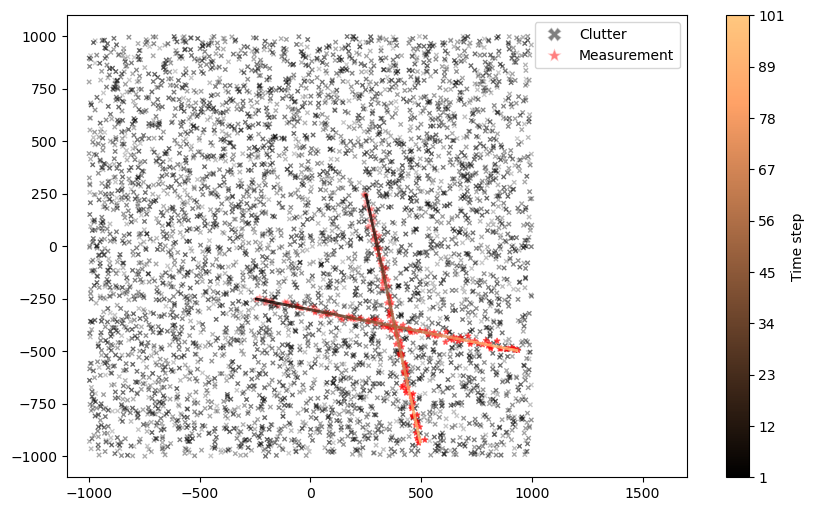
\includegraphics[width=\linewidth]{figures/c1-tracks-measurements.png}
    \end{subfigure}
    \hfill
    \begin{subfigure}[]{0.48\linewidth}
        \centering
        \begin{subfigure}[t]{\linewidth}
            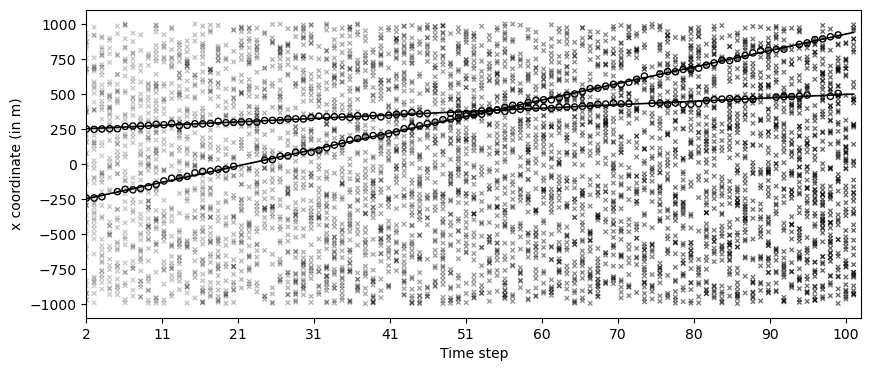
\includegraphics[width=\linewidth]{figures/c1-x-estimates.png}
        \end{subfigure}
        \vfill\par
        \begin{subfigure}[b]{\linewidth}
            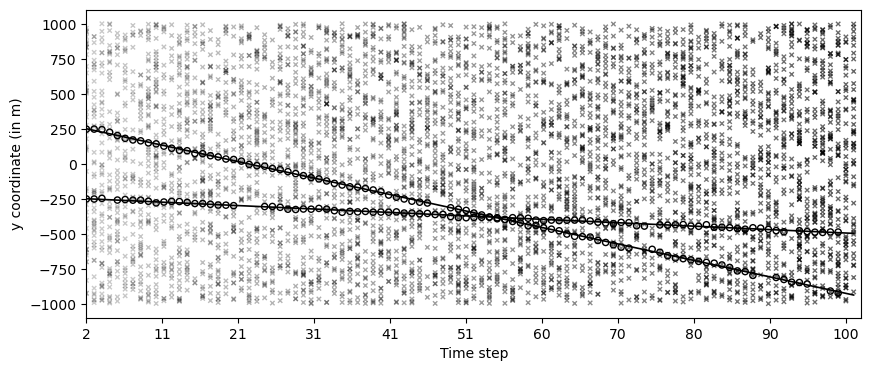
\includegraphics[width=\linewidth]{figures/c1-y-estimates.png}
        \end{subfigure}
    \end{subfigure}
  \caption[One sample of data and estimates for the (C1) scenario.]{One sample of data and estimates for the (C1) scenario. Left: True tracks of two objects (black to yellow) with clutter measurements (gray crosses) and received measurements (red stars) for a single Monte Carlo sample. Right: Change of both coordinates in time with noise measurements (red circles) and filter estimates (black circles) for the same Monte Carlo sample. The filter shows accurate estimates even in very cluttered environments.}
  \label{fig:c1-results-overview}
\end{figure*}

We can observe that the filter provides very accurate estimates even in cluttered environments. For instance, in this case, the filter receives an average of $50$ noise measurements for every measurement set. However, we also notice that estimates are not perfect. For instance, one of the objects did not receive estimates at time $k=21$ and it lasted for three time steps, and at $k=24$, the object appeared again.

Let us examine how changes in settings affect the filter performance in terms of metrics. To illustrate all runs for every parameter, we use a box plot. For every value of a parameter, we draw a box whose boundaries represent the first and third quartiles. The ``whiskers'' depict the minimum and maximum values of the distribution of metric values from all runs, and black dots represent those measurements that are considered outliers. The minimum and maximum values are calculated as one and a half times the interquartile range from the first and third quartiles, respectively, where the interquartile range is the difference between the two quartiles. Outliers are defined as those values that fall outside the range between the minimum and maximum. The black line inside boxes represents the median value, and the red dot is for the mean value. Means are connected to better see the overall trend. 

First, we examine the change of performance for different clutter rates. In Figure \ref{fig:c1-clutter}, we see that the increase of clutter measurements worsens the performance in both the precision of target estimates, and the estimate of the number of targets. It should be noted, that the increase in the expected absolute error is more pronounced than for the CPEP. It is clear that higher clutter rates causes more spurious estimates that the filter may consider to be real targets. Even in cases where these false tracks are not confirmed later, the number of estimated targets can be higher than the real number at a given time moment. However, in general, we see that the increase is not drastic, and the performance of the filter is good for even high values of the clutter rate.

\begin{figure}
    \centering
    \begin{subfigure}[]{0.48\linewidth}
        \centering
        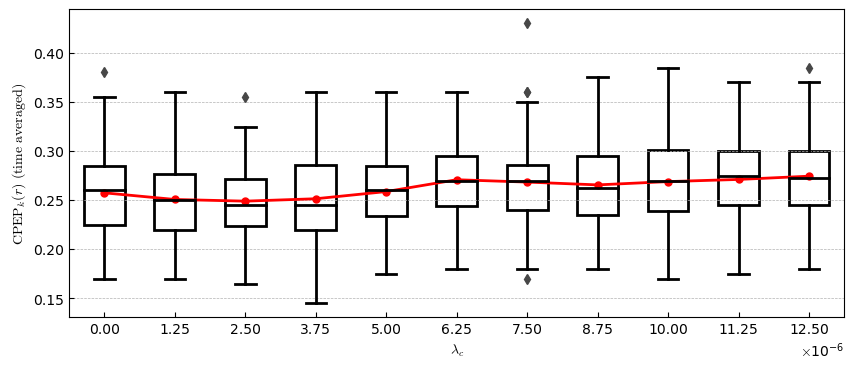
\includegraphics[width=\linewidth]{figures/c1-clutter-cpep.png}
    \end{subfigure}
    \hfill
    \begin{subfigure}[]{0.48\linewidth}
        \centering
        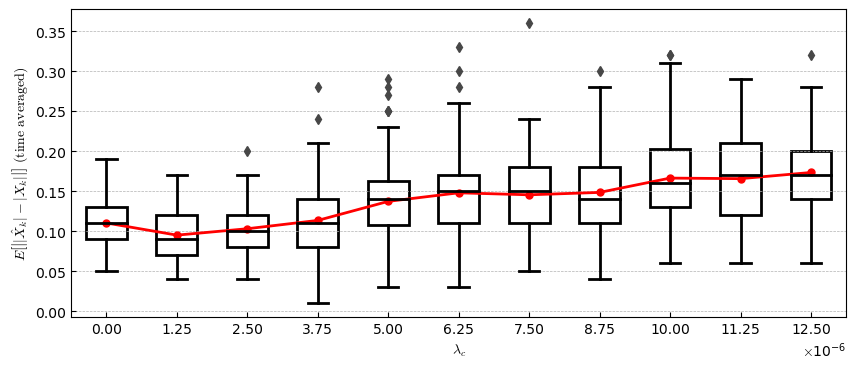
\includegraphics[width=\linewidth]{figures/c1-clutter-eae.png}
    \end{subfigure}
  \caption[(C1). Change of performance depending on the clutter rate.]{Here, we examine the change of CPEP (left) and the expected absolute error on the number of targets (right) for the (C1) scenario for different values of the clutter spatial rate $\lambda_c$. Every box is the representation of the distribution of $100$ independent samples. As the clutter spatial rate increases, the estimation error also increases, which may be observed on the growing trend of both metrics. All other setting are set to default values, i.e. $P_{D,k} = 0.98$, $P_{S,k} = 0.99$, $\tau = 10^{-5}$ and $U = 4$.}
  \label{fig:c1-clutter}
\end{figure}

Next, let us look how the filter behaves for different values of the detection probability. The detection probability is a parameter that may vary for different environments and sensors, and its setting may affect the overall tracking performance. Figure \ref{fig:c1-pd} shows how the estimation error changes for multiple settings of the detection probability. It can be seen that low detection probabilities influence the performance of the filter drastically in both the estimation of the number of targets and the precision of state estimates. For instance, the comparison of two values of $P_{D,k} = 0.7$ and $P_{D,k} = 1.0$ gives more than seven times better estimation results in terms of the number of targets and twice better results for the state estimation. This suggests that the GM-PHD filter may show poor results for higher clutter rates and lower detection probabilities.

\begin{figure}
    \centering
    \begin{subfigure}[]{0.48\linewidth}
        \centering
        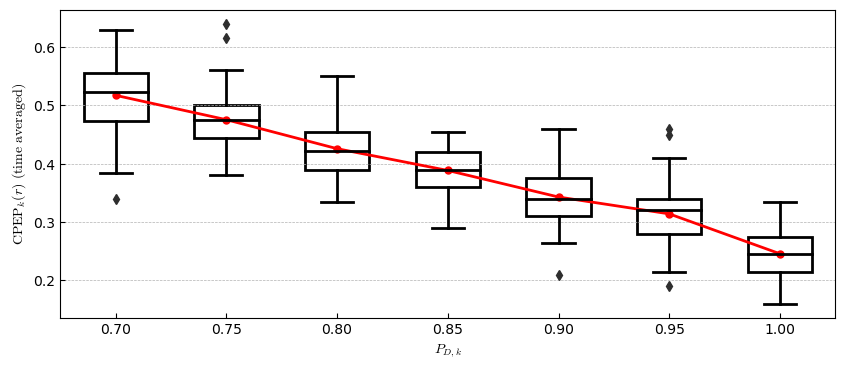
\includegraphics[width=\linewidth]{figures/c1-pd-cpep.png}
    \end{subfigure}
    \hfill
    \begin{subfigure}[]{0.48\linewidth}
        \centering
        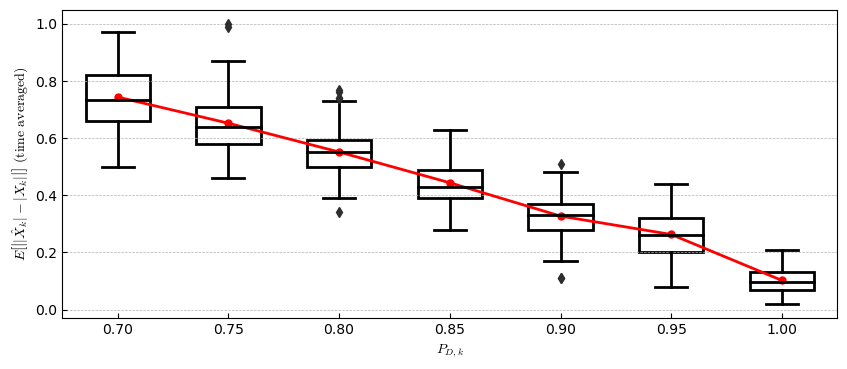
\includegraphics[width=\linewidth]{figures/c1-pd-eae.png}
    \end{subfigure}
  \caption[(C1). Change of performance depending on the detection probability.]{The change of CPEP (left) and the expected absolute error on the number of targets (right) for the (C1) scenario for different values of the detection probability $P_{D,k}$. Every box is the representation of the distribution of $100$ independent samples. As the detection probability increases, the estimation error decreases, which may be observed on the decreasing trend of both metrics. All other setting are set to default values, i.e. $\lambda_{c} = 12.5 \times 10^{-6}$, $P_{S,k} = 0.99$, $\tau = 10^{-5}$ and $U = 4$.}
  \label{fig:c1-pd}
\end{figure}

The third parameter we will examine is the probability of survival, $P_S$. In Figure \ref{fig:c1-ps}, we see that the performance is not affected by different values of the survival probability. The result suggests that even though the intensity of existing targets will rapidly decrease at every time step with a lower value of $P_{S,k}$, the tracks will still remain confirmed when the target generates enough measurements.

\begin{figure}
    \centering
    \begin{subfigure}[]{0.48\linewidth}
        \centering
        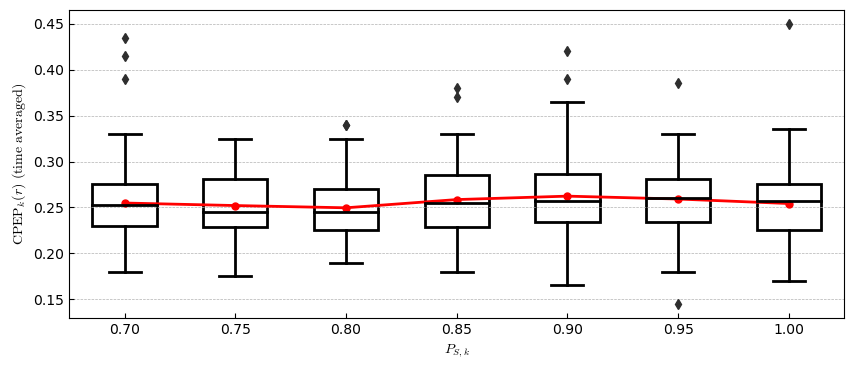
\includegraphics[width=\linewidth]{figures/c1-ps-cpep.png}
    \end{subfigure}
    \hfill
    \begin{subfigure}[]{0.48\linewidth}
        \centering
        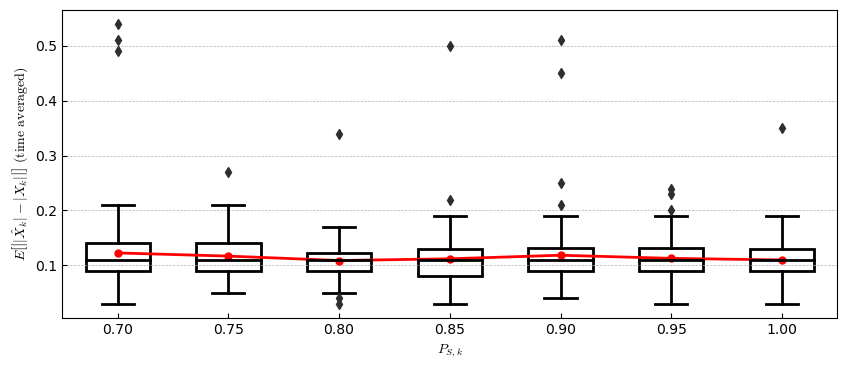
\includegraphics[width=\linewidth]{figures/c1-ps-eae.png}
    \end{subfigure}
  \caption[(C1). Change of performance depending on the survival probability.]{The change of CPEP (left) and the expected absolute error on the number of targets (right) for the (C1) scenario for different values of the survival probability $P_{S,k}$. Every box is the representation of the distribution of $100$ independent samples. Neither of metrics shows a change when the survival probability changes. All other setting are set to default values, i.e. $\lambda_{c} = 12.5 \times 10^{-6}$, $P_{D,k} = 0.98$, $\tau = 10^{-5}$ and $U = 4$.}
  \label{fig:c1-ps}
\end{figure}

The next variable parameter is the truncation threshold $\tau$. Figure \ref{fig:c1-tau} suggests that pruning too many components due to higher values of $\tau$ reduces the performance of the GM-PHD filter. For instance, $\tau = 10^{-3}$ caused a small decrease in both the precision and the estimate of the number of targets. The explanation of this effect is fairly straightforward. When the truncation threshold is too large, the number of hypotheses is drastically reduced at every time step and the loss of information in the posterior intensity is therefore not negligible.

\begin{figure}
    \centering
    \begin{subfigure}[]{0.48\linewidth}
        \centering
        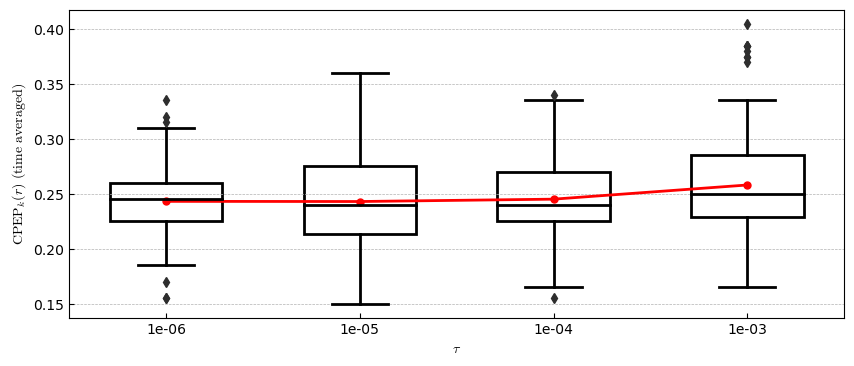
\includegraphics[width=\linewidth]{figures/c1-prune-cpep.png}
    \end{subfigure}
    \hfill
    \begin{subfigure}[]{0.48\linewidth}
        \centering
        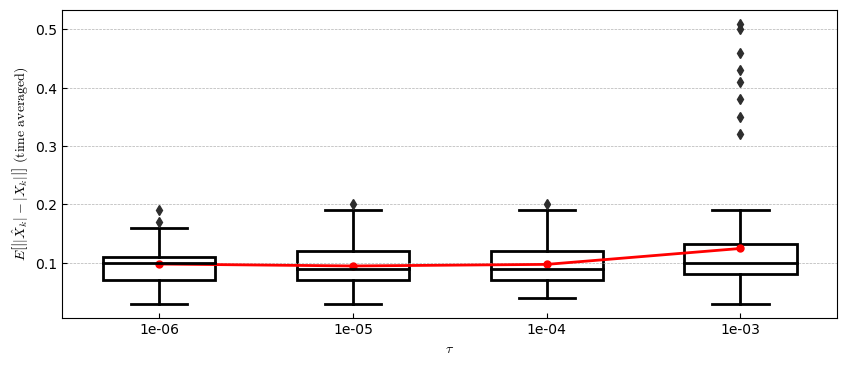
\includegraphics[width=\linewidth]{figures/c1-prune-eae.png}
    \end{subfigure}
  \caption[(C1). Change of performance depending on the prune threshold.]{The change of CPEP (left) and the expected absolute error on the number of targets (right) for the (C1) scenario for different values of the truncation threshold $\tau$. Every box is the representation of the distribution of $100$ independent samples. The X axis is on the logarithmic scale. We see, that, for higher values of $\tau$, the performance becomes worse. All other setting are set to default values, i.e. $\lambda_{c} = 12.5 \times 10^{-6}$, $P_{D,k} = 0.98$, $P_{S,k} = 0.99$ and $U = 4$.}
  \label{fig:c1-tau}
\end{figure}

The final parameter that was tested is the merge threshold $U$, or the maximum Mahalanobis distance between components on which these components will be merged into one. The results for different values of $U$ are shown in Figure \ref{fig:c1-u}. The increase in the distance between components causes the same effect as the increase of the truncation threshold $\tau$, that is, the loss of information from the posterior intensity. However, for this specific case and tested values of the parameter, the performance in both metrics worsens only slightly. The exact choice of the merge threshold $U$ is, however, domain-dependent.

\begin{figure}
    \centering
    \begin{subfigure}[]{0.48\linewidth}
        \centering
        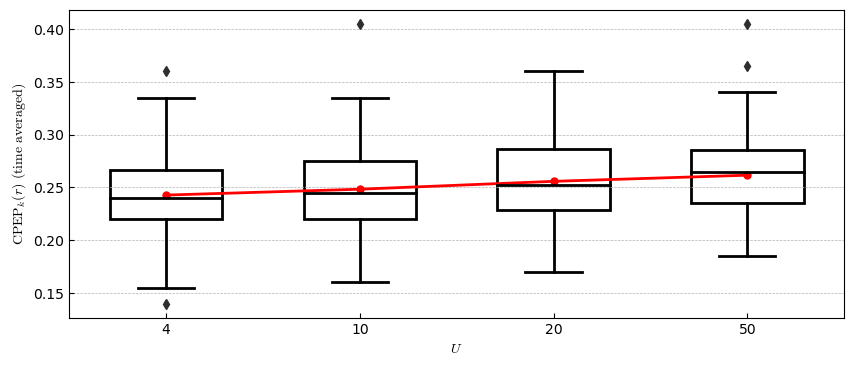
\includegraphics[width=\linewidth]{figures/c1-merge-cpep.png}
    \end{subfigure}
    \hfill
    \begin{subfigure}[]{0.48\linewidth}
        \centering
        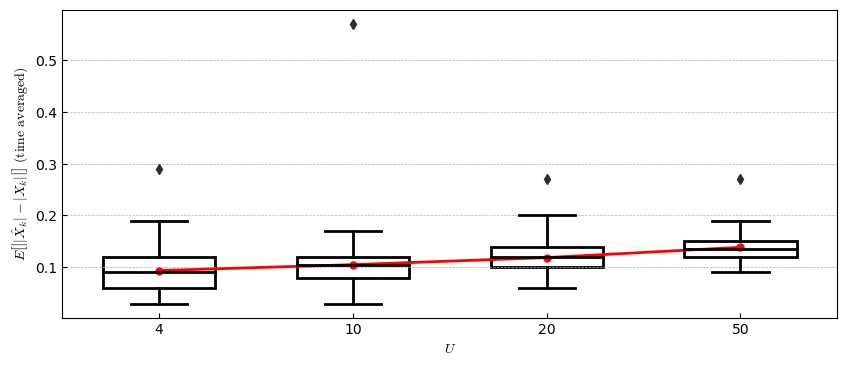
\includegraphics[width=\linewidth]{figures/c1-merge-eae.png}
    \end{subfigure}
  \caption[(C1). Change of performance depending on the merge threshold.]{The change of CPEP (left) and the expected absolute error on the number of targets (right) for the (C1) scenario for different values of the merge threshold $U$. Every box is the representation of the distribution of $100$ independent samples. The X axis does not have any scale. We see that, for higher values of $U$, the performance slightly worsens. All other settings are set to default values, i.e. $\lambda_{c} = 12.5 \times 10^{-6}$, $P_{D,k} = 0.98$, $P_{S,k} = 0.99$, and $\tau = 10^{-5}$.}
  \label{fig:c1-u}
\end{figure}

Finally, let us visually examine how trajectories are estimated and the final state of the posterior distribution. In Figure \ref{fig:c1-traj-post}, the left image illustrates the error in trajectory estimation. The track with the tag $667$ was terminated when two targets' paths cross each other, and the other track is created right after the intersection with a new tag $854$. We will later see how the effect of this problem worsens for more complex scenarios. However, we observe great results in terms of state estimation for both targets. The right image shows the internal state of the GM-PHD filter at time step $k=100$, more precisely the posterior intensity. It can be seen that two peaks are have expected value in the locations of two objects.

\begin{figure}
    \centering
    \begin{subfigure}[]{0.48\linewidth}
        \centering
        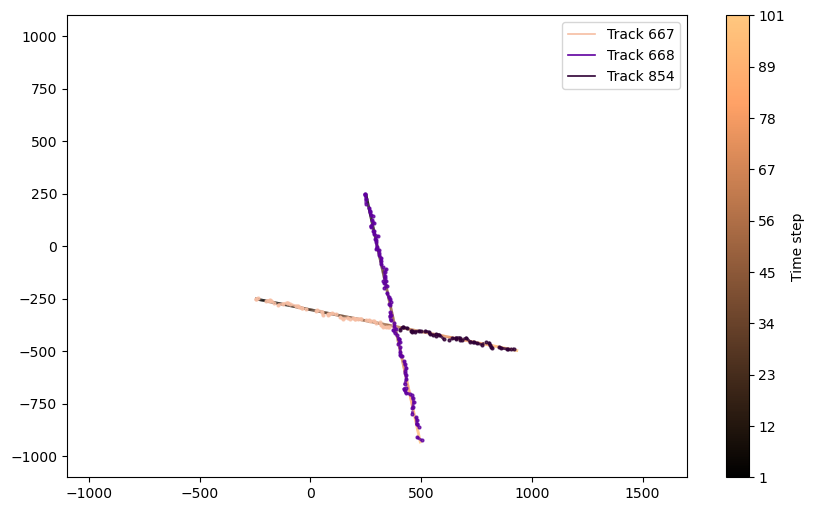
\includegraphics[width=\linewidth]{figures/c1-traj.png}
    \end{subfigure}
    \hfill
    \begin{subfigure}[]{0.48\linewidth}
        \centering
        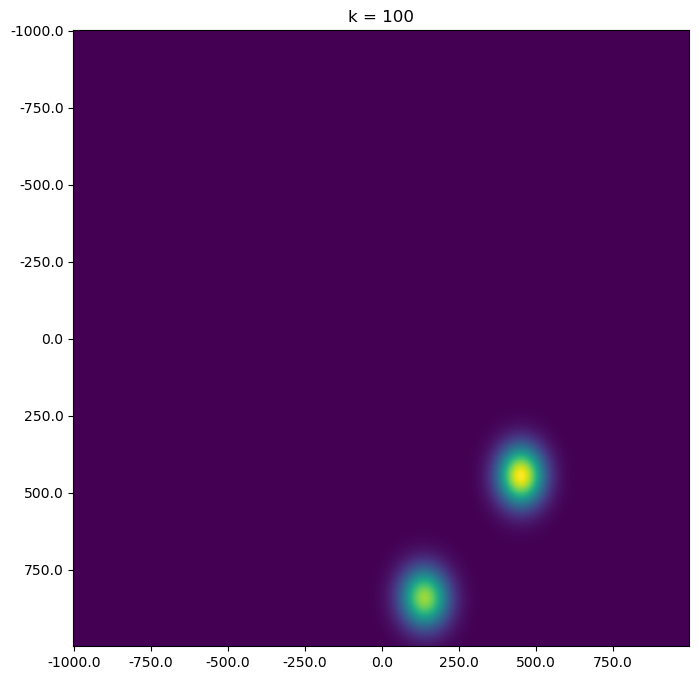
\includegraphics[width=\linewidth]{figures/c1-post.png}
    \end{subfigure}
  \caption[(C1). Trajectories estimations and the posterior intensity.]{Left: The visualization of trajectories estimates and the posterior distribution at time $k=100$. The straight gradient lines represent true tracks, the points represent state estimates generated by the GM-PHD filter, and different colors of the points illustrate unique tags of the estimated trajectories. Note, that when two tracks intersect, one of estimated tracks was falsely terminated and a new one created. Right: The posterior distribution at time step $k=100$. For visualization purposes, the covariance matrices of all Gaussian components were multiplied by the factor of $81$. Two Gaussian terms are visible on locations where two targets were at this time step. The bottom target has a lower weight, thus its color is dim. The filter was run with default settings, i.e. $\lambda_{c} = 12.5 \times 10^{-6}$, $P_{D,k} = 0.98$, $P_{S,k} = 0.99$, $\tau = 10^{-5}$, and $U=4$.}
  \label{fig:c1-traj-post}
\end{figure}

    \section{Test results (C2)}\label{sec:c2-results}
        % sample: clutter rate=50, best no. 014, worse no. 016

The second test scenario contains six independent objects that are born and die at different times. We have already discussed the influence of changing values over various parameters and will not include all the plots here, since every metric shows the exact same trend for all parameter values except for higher magnitudes of errors due to the increased number of objects. The reader can, however, find all figures in Appendix \ref{appendix:results-figures}. In this section, we will, however, compare two cases of trajectory estimation to point out the track continuity problem of the chosen tagging strategy.

First of all, let us examine the results of target state estimation of one sample, a worst-case scenario. In Figure \ref{fig:c2-results-overview}, we see how tracks, measurements, and clutter are generated along with state estimates depicted for two axes on the right side of the figure. We clearly see that for this exact sample there are many "holes" where the estimates were not suggested by the filter. One of the reasons for this behavior is false positive measurements that appear in close proximity to the real targets, which causes the filter to underestimate the likelihood of hypotheses of real target-to-measurement assignments.

\begin{figure*}
    \centering
    \begin{subfigure}[]{0.48\linewidth}
        \centering
        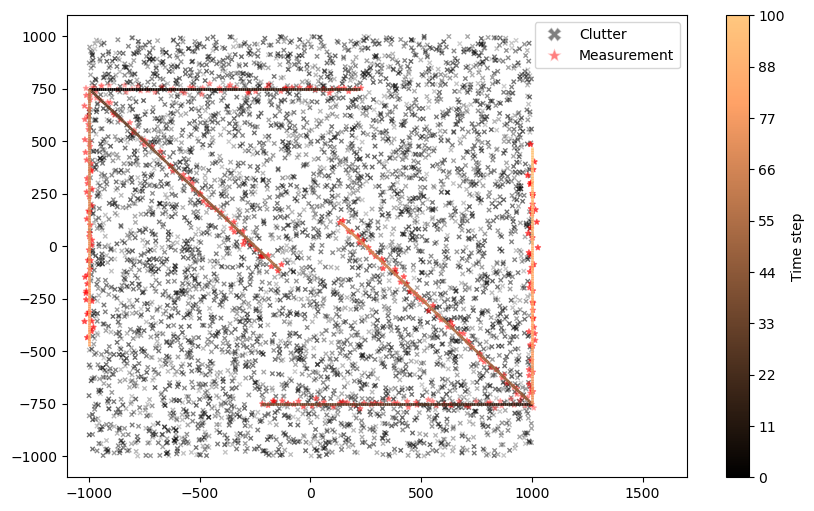
\includegraphics[width=\linewidth]{figures/c2-tracks-measurements.png}
    \end{subfigure}
    \hfill
    \begin{subfigure}[]{0.48\linewidth}
        \centering
        \begin{subfigure}[t]{\linewidth}
            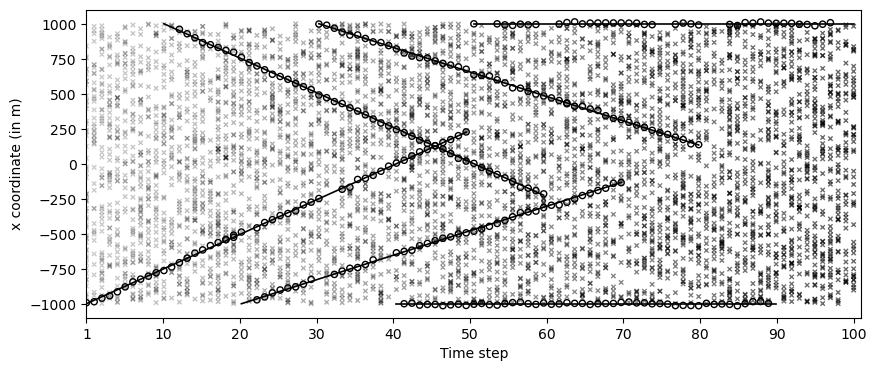
\includegraphics[width=\linewidth]{figures/c2-x-estimates.png}
        \end{subfigure}
        \vfill\par
        \begin{subfigure}[b]{\linewidth}
            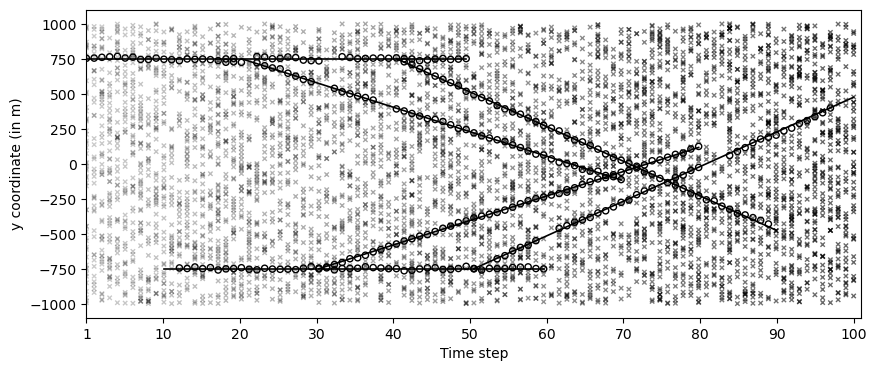
\includegraphics[width=\linewidth]{figures/c2-y-estimates.png}
        \end{subfigure}
    \end{subfigure}
  \caption[One sample of data and estimates for the (C2) scenario.]{One sample of data and estimates for the (C2) scenario. Left: True tracks of two objects (black to yellow) with clutter measurements (gray crosses) and received measurements (red stars) for a single Monte Carlo sample. Right: Change of both coordinates in time with noise measurements (red circles) and filter estimates (black circles) for the same Monte Carlo sample. In comparison to the (C1) scenario, the number of missed estimates is increased.}
  \label{fig:c2-results-overview}
\end{figure*}

The described behavior causes the track continuity problem already mentioned in the previous section. Figure \ref{fig:c2-track-continuity} compares two different runs on two different data samples. On the left picture, we see that there are six trajectory estimates for six targets, thus the estimate is correct. On the right image, however, the number of trajectories is higher, because tracks become terminated and new tracks are initialized. This is caused by the logic of tagging Gaussian components during merging. During this step of the GM-PHD filter, the component with the highest likelihood is chosen as the parent component, and other Gaussian terms are merged into the chosen one. If some new hypothesis created for a clutter measurement happens to have a higher weight, the Gaussian that had the initial tag is merged into this wrong component, and the correct tag disappears from the posterior intensity. The uncertainty in the posterior intensity is also shown in Figure \ref{fig:c2-post}. The best-case scenario is illustrated on the left. At time $k=100$, there is one target present in the scene, and the posterior intensity contains only one significant component. However, the bad scenario has a higher uncertainty in estimating the posterior PHD function, and we see several blobs in the image.

\begin{figure}
    \centering
    \begin{subfigure}[]{0.48\linewidth}
        \centering
        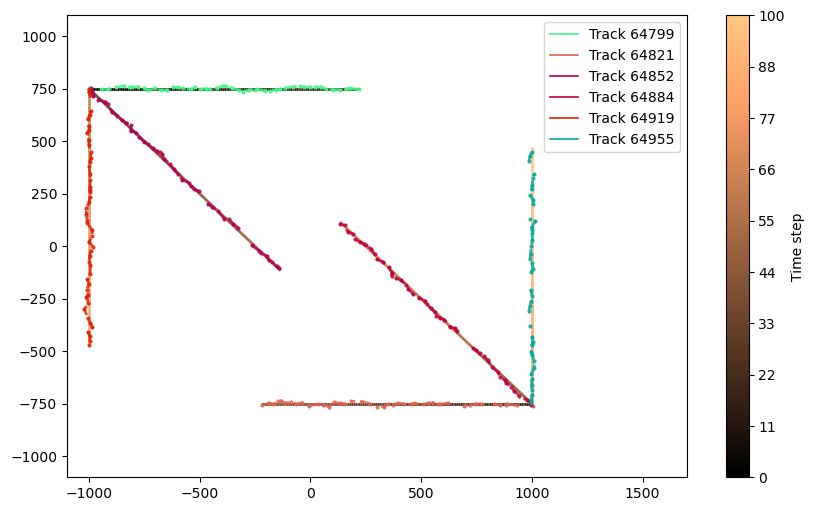
\includegraphics[width=\linewidth]{figures/c2-traj-good.png}
    \end{subfigure}
    \hfill
    \begin{subfigure}[]{0.48\linewidth}
        \centering
        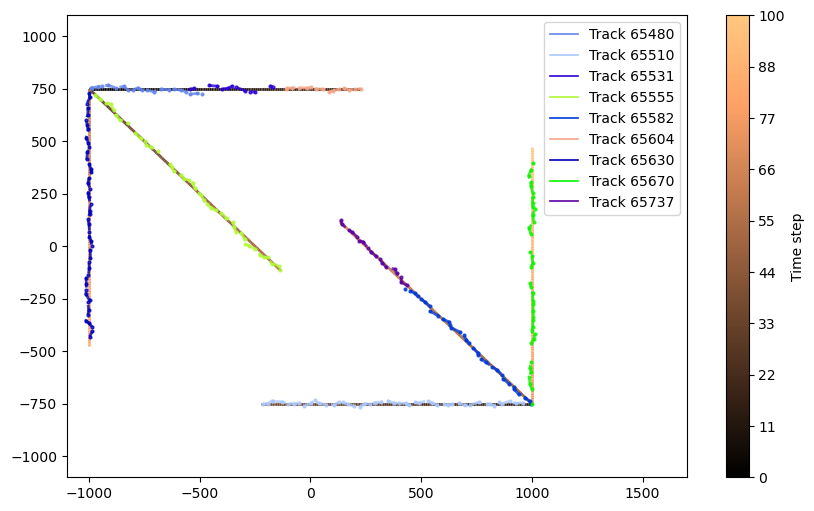
\includegraphics[width=\linewidth]{figures/c2-traj-bad.png}
    \end{subfigure}
  \caption[(C2). Comparison of trajectories estimates.]{Left: The visualization of trajectory estimates at time $k=100$ for the ideal case. For six targets, there are six different trajectories with good state estimates. Right: The same test scenario with wrong track estimates. We see that there are nine estimated trajectories, and the track continuity is not maintained. The filter was run with default settings, i.e., $\lambda_{c} = 12.5 \times 10^{-6}$, $P_{D,k} = 0.98$, $P_{S,k} = 0.99$, $\tau = 10^{-5}$, and $U=4$.}
  \label{fig:c2-track-continuity}
\end{figure}

\begin{figure}
    \centering
    \begin{subfigure}[]{0.48\linewidth}
        \centering
        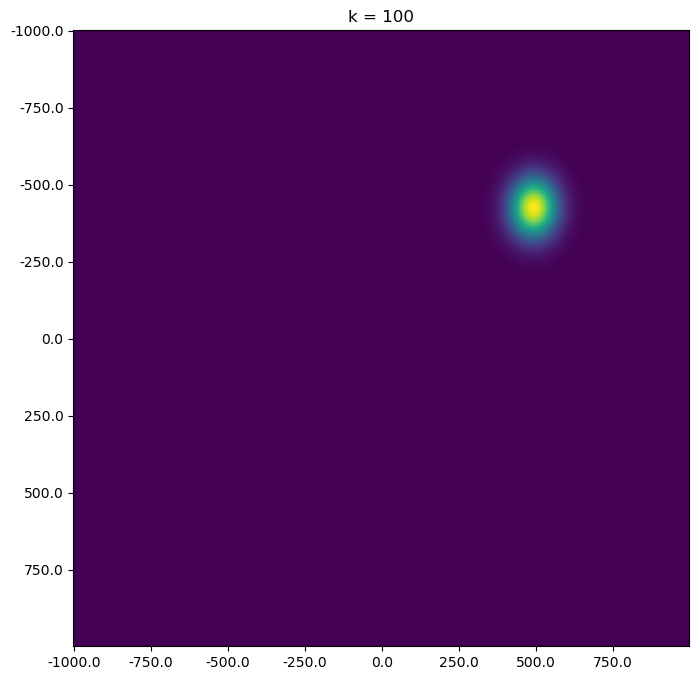
\includegraphics[width=\linewidth]{figures/c2-post-good.png}
    \end{subfigure}
    \hfill
    \begin{subfigure}[]{0.48\linewidth}
        \centering
        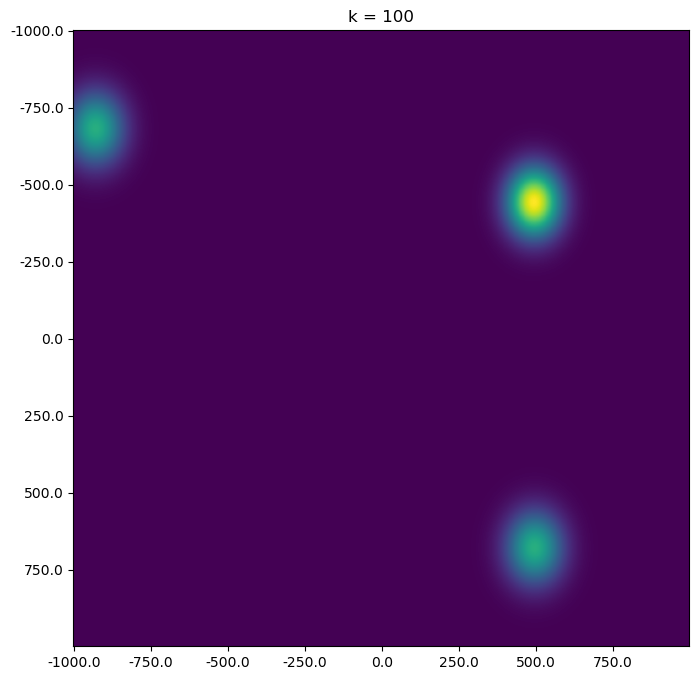
\includegraphics[width=\linewidth]{figures/c2-pos-bad.png}
    \end{subfigure}
  \caption[(C2). Comparison of posterior intensities for two cases.]{Left: The visualization of posterior intensity at time $k=100$. The intensity has only one Gaussian component with a high weight, which corresponds to the location of the only target present in the scene. Right: The posterior distribution at time step $k=100$ for a different sample of data. The uncertainty is higher, and there are three visible blobs for one existing target. Note that, for visualization purposes, the covariance matrices of all Gaussian components were multiplied by a factor of $81$. The filter was run with default settings, i.e. $\lambda_{c} = 12.5 \times 10^{-6}$, $P_{D,k} = 0.98$, $P_{S,k} = 0.99$, $\tau = 10^{-5}$, and $U=4$.}
  \label{fig:c2-post}
\end{figure}

    \section{Test results (C3)}\label{sec:c3-results}
        % sample: clutter rate=50, sample no. 008

The third case depicts the same scenario as (C2), however, with two additional targets that appear at unexpected locations. Figure \ref{fig:c3-results-overview} shows that the GM-PHD filter fails to estimate states of these two additional targets. On the right side of Figure, we see that there are no black circles for two lines on both the X axis, and the Y axis. The figures illustrating the change in metrics over different values of filter parameters is located in Appendix \ref{appendix:results-figures}.

\begin{figure*}
    \centering
    \begin{subfigure}[]{0.48\linewidth}
        \centering
        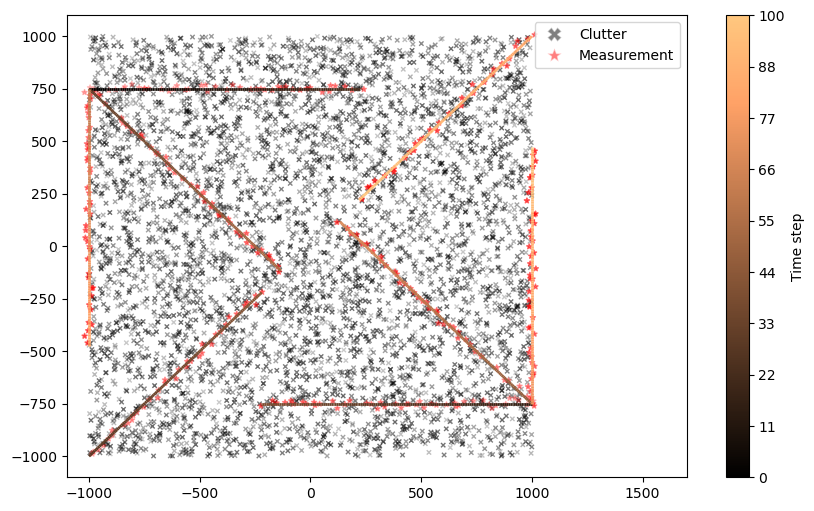
\includegraphics[width=\linewidth]{figures/c3-tracks-measurements.png}
    \end{subfigure}
    \hfill
    \begin{subfigure}[]{0.48\linewidth}
        \centering
        \begin{subfigure}[t]{\linewidth}
            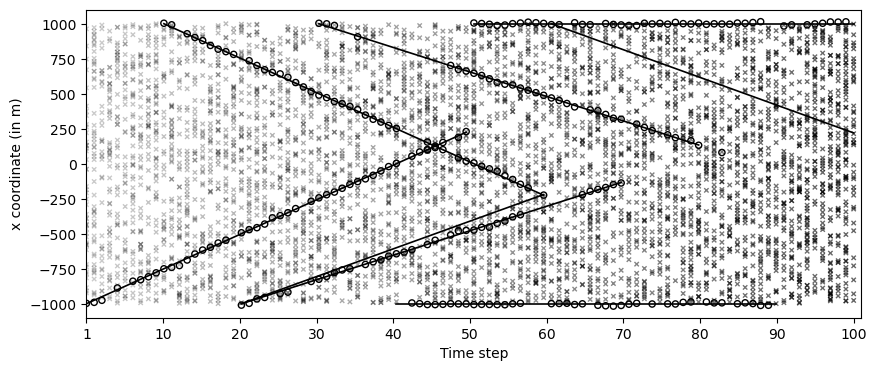
\includegraphics[width=\linewidth]{figures/c3-x-estimates.png}
        \end{subfigure}
        \vfill\par
        \begin{subfigure}[b]{\linewidth}
            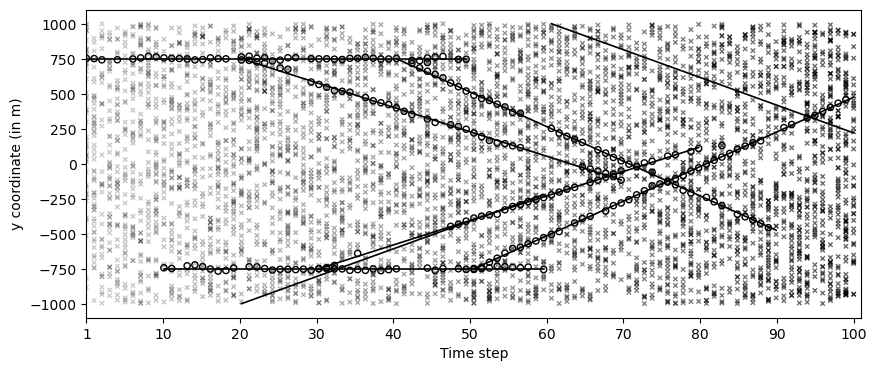
\includegraphics[width=\linewidth]{figures/c3-y-estimates.png}
        \end{subfigure}
    \end{subfigure}
  \caption[One sample of data and estimates for the (C3) scenario.]{One sample of data and estimates for the (C3) scenario. Left: True tracks of two objects (black to yellow) with clutter measurements (gray crosses) and received measurements (red stars) for a single Monte Carlo sample. Right: Change of both coordinates in time with noise measurements (red circles) and filter estimates (black circles) for the same Monte Carlo sample. Two targets were not detected by the filter, and no estimates were generated for them.}
  \label{fig:c3-results-overview}
\end{figure*}


If we look at Figure \ref{fig:c3-traj-post}, we will clearly see, that two targets starting from the bottom-left corner and the top-right corner were not detected by the filter. The track continuity problem persists. It should be noted, that for the demonstration purposes, we intentionally choose the sample where the track continuity problem is present and visible. Generally, the filter performs well, and the expected absolute error on the number of targets should be compared using the average value over all samples.

\begin{figure}
    \centering
    \begin{subfigure}[]{0.48\linewidth}
        \centering
        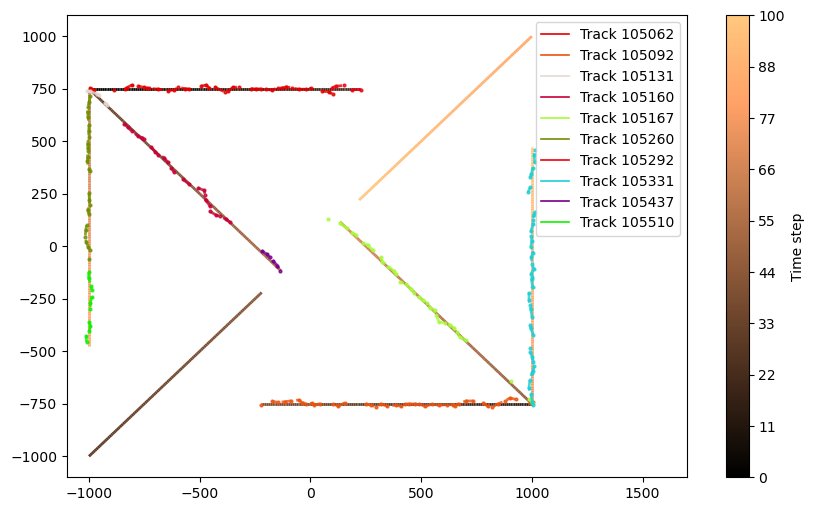
\includegraphics[width=\linewidth]{figures/c3-traj.png}
    \end{subfigure}
    \hfill
    \begin{subfigure}[]{0.48\linewidth}
        \centering
        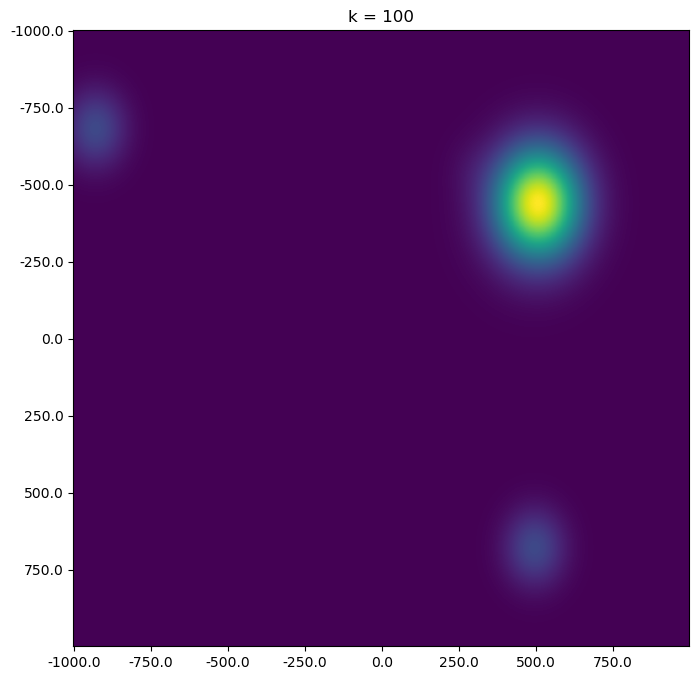
\includegraphics[width=\linewidth]{figures/c3-post.png}
    \end{subfigure}
  \caption[(C3). Trajectories estimations and the posterior intensity.]{Left: The visualization of trajectories estimates and the posterior distribution at time $k=100$. Two targets were not detected. Right: The posterior distribution at time step $k=100$. For visualization purposes, the covariance matrices of all Gaussian components were multiplied by the factor of $81$. The filter was run with default settings, i.e. $\lambda_{c} = 12.5 \times 10^{-6}$, $P_{D,k} = 0.98$, $P_{S,k} = 0.99$, $\tau = 10^{-5}$, and $U=4$.}
  \label{fig:c3-traj-post}
\end{figure}

    \section{Test results (C4)}\label{sec:c4-results}
        % sample: clutter rate=50, sample no. 097

Finally, we evaluate tracking results for the similar case as (C3) but with external information fusion. The tracking scenario with estimates generated by the GM-PHD filter is illustrated in Figure \ref{fig:c4-results-overview}. We can see that the filter now detects new targets and the estimates are precise even though the initial mean vectors and covariance matrices are not precise. 

\begin{figure*}
    \centering
    \begin{subfigure}[]{0.48\linewidth}
        \centering
        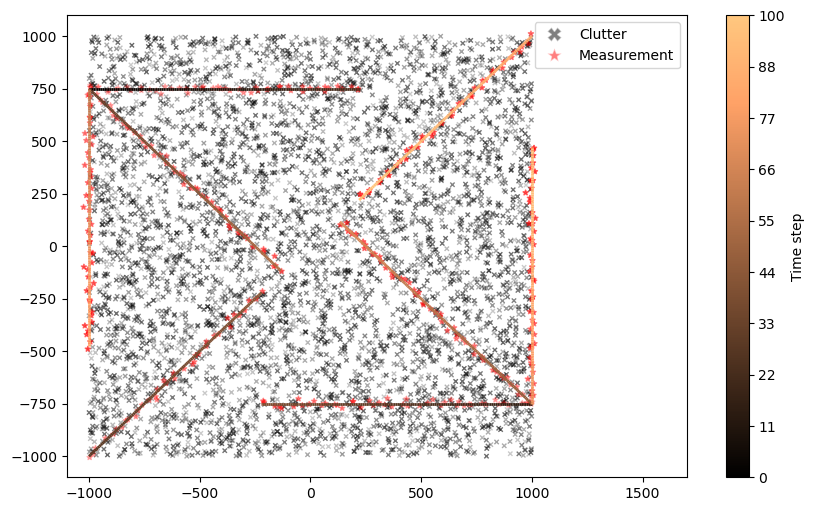
\includegraphics[width=\linewidth]{figures/c4-tracks-measurements.png}
    \end{subfigure}
    \hfill
    \begin{subfigure}[]{0.48\linewidth}
        \centering
        \begin{subfigure}[t]{\linewidth}
            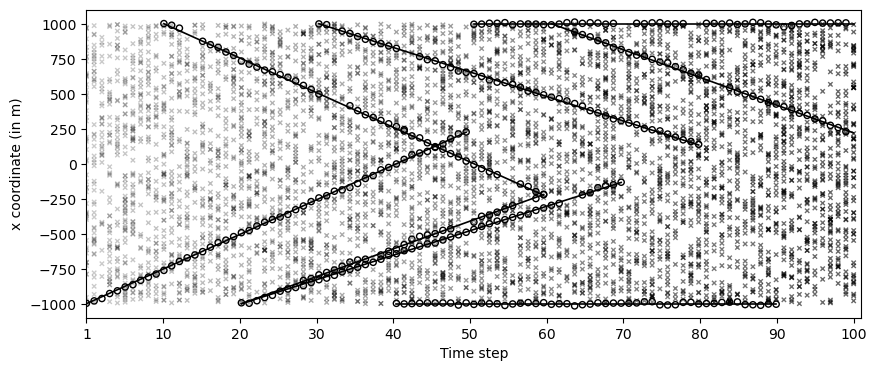
\includegraphics[width=\linewidth]{figures/c4-x-estimates.png}
        \end{subfigure}
        \vfill\par
        \begin{subfigure}[b]{\linewidth}
            \includegraphics[width=\linewidth]{figures/c4-y-estimates.png}
        \end{subfigure}
    \end{subfigure}
  \caption[One sample of data and estimates for the (C4) scenario.]{One sample of data and estimates for the (C4) scenario. Left: True tracks of two objects (black to yellow) with clutter measurements (gray crosses) and received measurements (red stars) for a single Monte Carlo sample. Right: Change of both coordinates in time with noise measurements (red circles) and filter estimates (black circles) for the same Monte Carlo sample. Two targets were not detected by the filter, and no estimates were generated for them.}
  \label{fig:c4-results-overview}
\end{figure*}

In Figure \ref{fig:c4-traj-post}, we see the same track continuity problem, where the filter created nine trajectories, while there are only eight targets. However, in comparison to the (C3) scenario, the objects are now detected, and their tracks are estimated correctly. Despite trajectory estimates being present, note that the filter required some time to start detecting the the bottom-left target. It is due to its large uncertainty and the small weight, their exact values are given in Section \ref{sec:c4-scenario}. Thus, the GM-PHD algorithm required several additional measurements to confirm the track.

\begin{figure}
    \centering
    \begin{subfigure}[]{0.48\linewidth}
        \centering
        \includegraphics[width=\linewidth]{figures/c4-traj.png}
    \end{subfigure}
    \hfill
    \begin{subfigure}[]{0.48\linewidth}
        \centering
        \includegraphics[width=\linewidth]{figures/c4-post.png}
    \end{subfigure}
  \caption[(C4). Trajectories estimations and the posterior intensity.]{Left: The visualization of trajectories estimates and the posterior distribution at time $k=100$. In comparison to the (C3) scenario, two targets are now detected correctly. Right: The posterior distribution at time step $k=100$. We see two Gaussian components that refer to two existing objects. For visualization purposes, the covariance matrices of all Gaussian components were multiplied by the factor of $81$. The filter was run with default settings, i.e. $\lambda_{c} = 12.5 \times 10^{-6}$, $P_{D,k} = 0.98$, $P_{S,k} = 0.99$, $\tau = 10^{-5}$, and $U=4$.}
  \label{fig:c4-traj-post}
\end{figure}

The visualization of all metrics for different filter settings is included in Appendix \ref{appendix:results-figures}. Here, we compare the evaluation of these metrics for default parameters in scenarios (C3) and (C4), as shown in Table \ref{table:c3-c4-metrics}.

\begin{table}
\begin{center}
\begin{tabular}{ | c || c | c | }
    \hline
            & CPEP              & EAE               \\ [0.5ex]
    \hline\hline
    (C3)    & 0.87876           & 0.85900           \\ 
    (C4)    & \textbf{0.85900}  & \textbf{0.35380}  \\ [1ex]
    \hline
\end{tabular}
\end{center}
\caption[Comparison of simulation results for the (C3) and (C4) scenarios.]{The comparison of CPEP and the expected absolute error on the number of targets (EAE) for the scenarios (C3) and (C4). The numbers represent the averaged values of metrics over $100$ Monte Carlo samples. The filter was run with default settings, i.e. $\lambda_{c} = 12.5 \times 10^{-6}$, $P_{D,k} = 0.98$, $P_{S,k} = 0.99$, $\tau = 10^{-5}$, and $U=4$.}\label{table:c3-c4-metrics}
\end{table}

    \section{Discussion}\label{sec:discussion}
        As we have presented the results of performance measurement, let us discuss them and draw several conclusions. In general, the GM-PHD filter is a robust algorithm. However, like any other algorithm, it has its drawbacks.

First of all, it is obvious that the filter is sensitive to the quality of data coming from a sensor. For instance, if the sensor has a low detection probability and high clutter rates, tracking performance may suffer from the uncertainty on both the state estimate precision and the estimated number of targets. Moreover, the filter becomes sensitive to the setting of the survival probability. For these cases, it is recommended to either use additional sources of information or use another tracking algorithm.

Secondly, let us discuss track maintenance. Generally, the GM-PHD filter has an in-built implicit track maintenance. When a Gaussian has a sufficient weight, in our case greater than $0.5$, the track is considered initialized and confirmed. However, there is a problem. If several clutter measurements happen to be in the vicinity of birth components, the likelihood of these components getting enough weights is quite high. This will lead to existence of tracks with only a few estimates, often only one. This problem may be addressed by increasing the minimum weight required for generating an estimate or by introducing some additional logic, such as the minimum number of estimates, something like the M/N logic discussed in Section \ref{sec:track-maintenance}.

The next problem is the consequence of the simple strategy we have chosen for tagging Gaussian components to connect estimates into trajectories. We have seen that it suffers from the track continuity problem, which is discussed in detail along with the reason in Section \ref{sec:c2-results}. We may try to address this issue by introducing more sophisticated techniques of track maintenance. For instance, we could track the history of track estimates for each tag, and if the correct tag would have been discarded in favor of a tag with an empty history, we would detect it and assign the correct tag to preserve the track continuity. The other option would be to use clustering techniques like in the JPDA filter.

Next, we have observed the change of performance when there are no fusion components. They are fundamentally similar to birth components, but we have shown how they could be used for inputting additional external information into the filter. For blind zones, there is no way to append information using the standard techniques. The filter is unable to capture targets that are invisible to a sensor, and the way how the posterior intensity is represented in the GM-PHD filter makes it impossible to confirm tracks since there are no Gaussian terms to which new measurements can be assigned. We could have defined the birth components that cover the whole field of view, however, it would lead to the problem discussed in the previous paragraph, i.e., too many false estimates because of confirming birth components with clutter measurements.

Last but not least, it is obvious that the complexity $\mathcal{O}(mn)$ discussed in Section \ref{sec:phd-filter} assumes that the computational burden of the GM-PHD filter is highly dependent on the clutter rate. If there are too many false positive measurements at each time step, the performance in terms of processing time degrades. This is another reason why it is required to reduce the clutter rate as much as possible.

Despite all the drawbacks we have discussed, the GM-PHD filter remains one of the most popular and robust solutions to multi-target tracking. The filter is fast and reliable; it does not need to estimate the full posterior distribution, which is often complex. For Gaussian-linear cases, the GM-PHD filter has a closed form solution, and non-linear models can be estimated using the UK-PHD or the EK-PHD filter.


%%%%%%%%%%%%%%%%%%%%%%%%%%%%%%%%%%%%%%%%%%
% Conclusion
%%%%%%%%%%%%%%%%%%%%%%%%%%%%%%%%%%%%%%%%%%
\chapter{Conclusion}In this work, we explored one of the most popular Bayesian filters for multi-target tracking in Gaussian-linear cases, the Gaussian Mixture Probability Density (GM-PHD) filter. We investigated its performance and robustness in several tracking scenarios, including challenging situations where a sensor fails to collect measurements from targets and external information fusion is required.

We have demonstrated that the performance of the GM-PHD filter can be improved by incorporating external estimates from other sensors, as shown through evaluation of several metrics that indicated significant improvement in tracking results.

However, we have also identified a problem with track continuity when using the simple tagging of Gaussian components. We believe that more sophisticated techniques may improve track maintenance of the GM-PHD filter and make it more robust to complex scenarios with high uncertainty due to clutter measurements and a high number of targets.

Additionally, we have measured and discussed the filter's performance depending on the setup of internal parameters. We observed that the GM-PHD filter was sensitive to the choice of settings, particularly the clutter rate and probability of detection, highlighting the need to consider environmental conditions and the quality of the sensor when using the filter.

In conclusion, the GM-PHD filter remains a powerful and robust algorithm for state estimation of multiple targets in complex scenarios. Its computational complexity is outstanding compared to traditional multi-target tracking algorithms, and it is proven that the propagation of only the posterior first-order moment may be sufficient to achieve good tracking results. We believe that the techniques introduced in this work and the comprehensive performance measurements conducted may aid the multi-tracking research community in further improving the GM-PHD filter.


%%%%%%%%%%%%%%%%%%%%%%%%%%%%%%%%%%%%%%%%%%
% Appendices
%%%%%%%%%%%%%%%%%%%%%%%%%%%%%%%%%%%%%%%%%%

\appendix\appendixinit
\chapter{Appendix 1. Results comparison across different filter parameters}\label{appendix:results-figures}
    In this appendix, we present all testing results for the scenarios described in the main text. The results for each testing case are similar to those presented in Section \ref{sec:c1-results}; however, the reader may find it helpful to review the measurements for other test cases. Figures \ref{fig:c2-clutter}, \ref{fig:c3-clutter}, and \ref{fig:c4-clutter} show the change of metrics depending on the change of the clutter spatial rate $\lambda_c$ for scenarios (C2), (C3), and (C4), respectively. Figures \ref{fig:c2-pd}, \ref{fig:c3-pd}, and \ref{fig:c4-pd} depict the change of metrics for different values of the detection probability $P_{D,k}$ for each individual case in the same order. Figures \ref{fig:c2-ps}, \ref{fig:c3-ps}, and \ref{fig:c4-ps} show the change for the survival probability $P_{S,k}$, Figures \ref{fig:c2-tau}, \ref{fig:c3-tau}, and \ref{fig:c4-tau} for the truncation threshold $\tau$, and finally, Figures \ref{fig:c2-u}, \ref{fig:c3-u}, and \ref{fig:c4-u} for the merge threshold $U$ for scenarios (C2), (C3), and (C4), respectively. All figures are ordered in a way in which metrics for one parameter are grouped together so that the reader can compare results for different test cases. Every figure is provided with a detailed description of what it depicts.

\newpage  % three figures per page, otherwise one is placed under the par above

%%%%%%%%%%%%%%%%%%%%%%%%%%%%%%%%%%%%%%%%%%%%%%%%
% Clutter rate
%%%%%%%%%%%%%%%%%%%%%%%%%%%%%%%%%%%%%%%%%%%%%%%%

\begin{figure}
    \centering
    \begin{subfigure}[]{0.48\linewidth}
        \centering
        \includegraphics[width=\linewidth]{figures/c2-clutter-cpep.png}
    \end{subfigure}
    \hfill
    \begin{subfigure}[]{0.48\linewidth}
        \centering
        \includegraphics[width=\linewidth]{figures/c2-clutter-eae.png}
    \end{subfigure}
  \caption[(C2). Change of performance depending on the clutter rate.]{Here, we examine the change of CPEP (left) and the expected absolute error on the number of targets (right) for the (C2) scenario for different values of the clutter spatial rate $\lambda_c$. Every box is the representation of the distribution of $100$ independent samples. As the clutter spatial rate increases, the estimation error also increases, which may be observed on the growing trend of both metrics. All other setting are set to default values, i.e. $P_{D,k} = 0.98$, $P_{S,k} = 0.99$, $\tau = 10^{-5}$ and $U = 4$.}
  \label{fig:c2-clutter}
\end{figure}

\begin{figure}
    \centering
    \begin{subfigure}[]{0.48\linewidth}
        \centering
        \includegraphics[width=\linewidth]{figures/c3-clutter-cpep.png}
    \end{subfigure}
    \hfill
    \begin{subfigure}[]{0.48\linewidth}
        \centering
        \includegraphics[width=\linewidth]{figures/c3-clutter-eae.png}
    \end{subfigure}
  \caption[(C3). Change of performance depending on the clutter rate.]{Here, we examine the change of CPEP (left) and the expected absolute error on the number of targets (right) for the (C3) scenario for different values of the clutter spatial rate $\lambda_c$. Every box is the representation of the distribution of $100$ independent samples. As the clutter spatial rate increases, the estimation error also increases, which may be observed on the growing trend of both metrics. All other setting are set to default values, i.e. $P_{D,k} = 0.98$, $P_{S,k} = 0.99$, $\tau = 10^{-5}$ and $U = 4$.}
  \label{fig:c3-clutter}
\end{figure}

\begin{figure}
    \centering
    \begin{subfigure}[]{0.48\linewidth}
        \centering
        \includegraphics[width=\linewidth]{figures/c4-clutter-cpep.png}
    \end{subfigure}
    \hfill
    \begin{subfigure}[]{0.48\linewidth}
        \centering
        \includegraphics[width=\linewidth]{figures/c4-clutter-eae.png}
    \end{subfigure}
  \caption[(C4). Change of performance depending on the clutter rate.]{Here, we examine the change of CPEP (left) and the expected absolute error on the number of targets (right) for the (C4) scenario for different values of the clutter spatial rate $\lambda_c$. Every box is the representation of the distribution of $100$ independent samples. As the clutter spatial rate increases, the estimation error also increases, which may be observed on the growing trend of both metrics. All other setting are set to default values, i.e. $P_{D,k} = 0.98$, $P_{S,k} = 0.99$, $\tau = 10^{-5}$ and $U = 4$.}
  \label{fig:c4-clutter}
\end{figure}

%%%%%%%%%%%%%%%%%%%%%%%%%%%%%%%%%%%%%%%%%%%%%%%%
% Probability of detection
%%%%%%%%%%%%%%%%%%%%%%%%%%%%%%%%%%%%%%%%%%%%%%%%

\begin{figure}
    \centering
    \begin{subfigure}[]{0.48\linewidth}
        \centering
        \includegraphics[width=\linewidth]{figures/c2-pd-cpep.png}
    \end{subfigure}
    \hfill
    \begin{subfigure}[]{0.48\linewidth}
        \centering
        \includegraphics[width=\linewidth]{figures/c2-pd-eae.png}
    \end{subfigure}
  \caption[(C2). Change of performance depending on the detection probability.]{The change of CPEP (left) and the expected absolute error on the number of targets (right) for the (C2) scenario for different values of the detection probability $P_{D,k}$. Every box is the representation of the distribution of $100$ independent samples. As the detection probability increases, the estimation error decreases, which may be observed on the decreasing trend of both metrics. All other setting are set to default values, i.e. $\lambda_{c} = 12.5 \times 10^{-6}$, $P_{S,k} = 0.99$, $\tau = 10^{-5}$ and $U = 4$.}
  \label{fig:c2-pd}
\end{figure}

\begin{figure}
    \centering
    \begin{subfigure}[]{0.48\linewidth}
        \centering
        \includegraphics[width=\linewidth]{figures/c3-pd-cpep.png}
    \end{subfigure}
    \hfill
    \begin{subfigure}[]{0.48\linewidth}
        \centering
        \includegraphics[width=\linewidth]{figures/c3-pd-eae.png}
    \end{subfigure}
  \caption[(C3). Change of performance depending on the detection probability.]{The change of CPEP (left) and the expected absolute error on the number of targets (right) for the (C3) scenario for different values of the detection probability $P_{D,k}$. Every box is the representation of the distribution of $100$ independent samples. As the detection probability increases, the estimation error decreases, which may be observed on the decreasing trend of both metrics. All other setting are set to default values, i.e. $\lambda_{c} = 12.5 \times 10^{-6}$, $P_{S,k} = 0.99$, $\tau = 10^{-5}$ and $U = 4$.}
  \label{fig:c3-pd}
\end{figure}

\begin{figure}
    \centering
    \begin{subfigure}[]{0.48\linewidth}
        \centering
        \includegraphics[width=\linewidth]{figures/c4-pd-cpep.png}
    \end{subfigure}
    \hfill
    \begin{subfigure}[]{0.48\linewidth}
        \centering
        \includegraphics[width=\linewidth]{figures/c4-pd-eae.png}
    \end{subfigure}
  \caption[(C4). Change of performance depending on the detection probability.]{The change of CPEP (left) and the expected absolute error on the number of targets (right) for the (C4) scenario for different values of the detection probability $P_{D,k}$. Every box is the representation of the distribution of $100$ independent samples. As the detection probability increases, the estimation error decreases, which may be observed on the decreasing trend of both metrics. All other setting are set to default values, i.e. $\lambda_{c} = 12.5 \times 10^{-6}$, $P_{S,k} = 0.99$, $\tau = 10^{-5}$ and $U = 4$.}
  \label{fig:c4-pd}
\end{figure}

%%%%%%%%%%%%%%%%%%%%%%%%%%%%%%%%%%%%%%%%%%%%%%%%
% Probability of survival
%%%%%%%%%%%%%%%%%%%%%%%%%%%%%%%%%%%%%%%%%%%%%%%%

\begin{figure}
    \centering
    \begin{subfigure}[]{0.48\linewidth}
        \centering
        \includegraphics[width=\linewidth]{figures/c2-ps-cpep.png}
    \end{subfigure}
    \hfill
    \begin{subfigure}[]{0.48\linewidth}
        \centering
        \includegraphics[width=\linewidth]{figures/c2-ps-eae.png}
    \end{subfigure}
  \caption[(C2). Change of performance depending on the survival probability.]{The change of CPEP (left) and the expected absolute error on the number of targets (right) for the (C2) scenario for different values of the survival probability $P_{S,k}$. Every box is the representation of the distribution of $100$ independent samples. Neither of metrics shows a change when the survival probability changes. All other setting are set to default values, i.e. $\lambda_{c} = 12.5 \times 10^{-6}$, $P_{D,k} = 0.98$, $\tau = 10^{-5}$ and $U = 4$.}
  \label{fig:c2-ps}
\end{figure}

\begin{figure}
    \centering
    \begin{subfigure}[]{0.48\linewidth}
        \centering
        \includegraphics[width=\linewidth]{figures/c3-ps-cpep.png}
    \end{subfigure}
    \hfill
    \begin{subfigure}[]{0.48\linewidth}
        \centering
        \includegraphics[width=\linewidth]{figures/c3-ps-eae.png}
    \end{subfigure}
  \caption[(C3). Change of performance depending on the survival probability.]{The change of CPEP (left) and the expected absolute error on the number of targets (right) for the (C3) scenario for different values of the survival probability $P_{S,k}$. Every box is the representation of the distribution of $100$ independent samples. Neither of metrics shows a change when the survival probability changes. All other setting are set to default values, i.e. $\lambda_{c} = 12.5 \times 10^{-6}$, $P_{D,k} = 0.98$, $\tau = 10^{-5}$ and $U = 4$.}
  \label{fig:c3-ps}
\end{figure}

\begin{figure}
    \centering
    \begin{subfigure}[]{0.48\linewidth}
        \centering
        \includegraphics[width=\linewidth]{figures/c4-ps-cpep.png}
    \end{subfigure}
    \hfill
    \begin{subfigure}[]{0.48\linewidth}
        \centering
        \includegraphics[width=\linewidth]{figures/c4-ps-eae.png}
    \end{subfigure}
  \caption[(C4). Change of performance depending on the survival probability.]{The change of CPEP (left) and the expected absolute error on the number of targets (right) for the (C4) scenario for different values of the survival probability $P_{S,k}$. Every box is the representation of the distribution of $100$ independent samples. Neither of metrics shows a change when the survival probability changes. All other setting are set to default values, i.e. $\lambda_{c} = 12.5 \times 10^{-6}$, $P_{D,k} = 0.98$, $\tau = 10^{-5}$ and $U = 4$.}
  \label{fig:c4-ps}
\end{figure}

%%%%%%%%%%%%%%%%%%%%%%%%%%%%%%%%%%%%%%%%%%%%%%%%
% Truncation threshold
%%%%%%%%%%%%%%%%%%%%%%%%%%%%%%%%%%%%%%%%%%%%%%%%

\begin{figure}
    \centering
    \begin{subfigure}[]{0.48\linewidth}
        \centering
        \includegraphics[width=\linewidth]{figures/c2-tau-cpep.png}
    \end{subfigure}
    \hfill
    \begin{subfigure}[]{0.48\linewidth}
        \centering
        \includegraphics[width=\linewidth]{figures/c2-tau-eae.png}
    \end{subfigure}
  \caption[(C2). Change of performance depending on the prune threshold.]{The change of CPEP (left) and the expected absolute error on the number of targets (right) for the (C2) scenario for different values of the truncation threshold $\tau$. Every box is the representation of the distribution of $100$ independent samples. The X axis is on the logarithmic scale. We see, that, for higher values of $\tau$, the performance becomes worse. All other setting are set to default values, i.e. $\lambda_{c} = 12.5 \times 10^{-6}$, $P_{D,k} = 0.98$, $P_{S,k} = 0.99$ and $U = 4$.}
  \label{fig:c2-tau}
\end{figure}

\begin{figure}
    \centering
    \begin{subfigure}[]{0.48\linewidth}
        \centering
        \includegraphics[width=\linewidth]{figures/c3-tau-cpep.png}
    \end{subfigure}
    \hfill
    \begin{subfigure}[]{0.48\linewidth}
        \centering
        \includegraphics[width=\linewidth]{figures/c3-tau-eae.png}
    \end{subfigure}
  \caption[(C3). Change of performance depending on the prune threshold.]{The change of CPEP (left) and the expected absolute error on the number of targets (right) for the (C3) scenario for different values of the truncation threshold $\tau$. Every box is the representation of the distribution of $100$ independent samples. The X axis is on the logarithmic scale. We see, that, for higher values of $\tau$, the performance becomes worse. All other setting are set to default values, i.e. $\lambda_{c} = 12.5 \times 10^{-6}$, $P_{D,k} = 0.98$, $P_{S,k} = 0.99$ and $U = 4$.}
  \label{fig:c3-tau}
\end{figure}

\begin{figure}
    \centering
    \begin{subfigure}[]{0.48\linewidth}
        \centering
        \includegraphics[width=\linewidth]{figures/c4-tau-cpep.png}
    \end{subfigure}
    \hfill
    \begin{subfigure}[]{0.48\linewidth}
        \centering
        \includegraphics[width=\linewidth]{figures/c4-tau-eae.png}
    \end{subfigure}
  \caption[(C4). Change of performance depending on the prune threshold.]{The change of CPEP (left) and the expected absolute error on the number of targets (right) for the (C4) scenario for different values of the truncation threshold $\tau$. Every box is the representation of the distribution of $100$ independent samples. The X axis is on the logarithmic scale. We see, that, for higher values of $\tau$, the performance becomes worse. All other setting are set to default values, i.e. $\lambda_{c} = 12.5 \times 10^{-6}$, $P_{D,k} = 0.98$, $P_{S,k} = 0.99$ and $U = 4$.}
  \label{fig:c4-tau}
\end{figure}

%%%%%%%%%%%%%%%%%%%%%%%%%%%%%%%%%%%%%%%%%%%%%%%%
% Merge threshold
%%%%%%%%%%%%%%%%%%%%%%%%%%%%%%%%%%%%%%%%%%%%%%%%

\begin{figure}
    \centering
    \begin{subfigure}[]{0.48\linewidth}
        \centering
        \includegraphics[width=\linewidth]{figures/c2-u-cpep.png}
    \end{subfigure}
    \hfill
    \begin{subfigure}[]{0.48\linewidth}
        \centering
        \includegraphics[width=\linewidth]{figures/c2-u-eae.png}
    \end{subfigure}
  \caption[(C2). Change of performance depending on the merge threshold.]{The change of CPEP (left) and the expected absolute error on the number of targets (right) for the (C2) scenario for different values of the merge threshold $U$. Every box is the representation of the distribution of $100$ independent samples. The X axis does not have any scale. We see that, for higher values of $U$, the performance slightly worsens. All other settings are set to default values, i.e. $\lambda_{c} = 12.5 \times 10^{-6}$, $P_{D,k} = 0.98$, $P_{S,k} = 0.99$, and $\tau = 10^{-5}$.}
  \label{fig:c2-u}
\end{figure}

\begin{figure}
    \centering
    \begin{subfigure}[]{0.48\linewidth}
        \centering
        \includegraphics[width=\linewidth]{figures/c3-u-cpep.png}
    \end{subfigure}
    \hfill
    \begin{subfigure}[]{0.48\linewidth}
        \centering
        \includegraphics[width=\linewidth]{figures/c3-u-eae.png}
    \end{subfigure}
  \caption[(C3). Change of performance depending on the merge threshold.]{The change of CPEP (left) and the expected absolute error on the number of targets (right) for the (C3) scenario for different values of the merge threshold $U$. Every box is the representation of the distribution of $100$ independent samples. The X axis does not have any scale. We see that, for higher values of $U$, the performance slightly worsens. All other settings are set to default values, i.e. $\lambda_{c} = 12.5 \times 10^{-6}$, $P_{D,k} = 0.98$, $P_{S,k} = 0.99$, and $\tau = 10^{-5}$.}
  \label{fig:c3-u}
\end{figure}

\begin{figure}
    \centering
    \begin{subfigure}[]{0.48\linewidth}
        \centering
        \includegraphics[width=\linewidth]{figures/c4-u-cpep.png}
    \end{subfigure}
    \hfill
    \begin{subfigure}[]{0.48\linewidth}
        \centering
        \includegraphics[width=\linewidth]{figures/c4-u-eae.png}
    \end{subfigure}
  \caption[(C4). Change of performance depending on the merge threshold.]{The change of CPEP (left) and the expected absolute error on the number of targets (right) for the (C4) scenario for different values of the merge threshold $U$. Every box is the representation of the distribution of $100$ independent samples. The X axis does not have any scale. We see that, for higher values of $U$, the performance slightly worsens. All other settings are set to default values, i.e. $\lambda_{c} = 12.5 \times 10^{-6}$, $P_{D,k} = 0.98$, $P_{S,k} = 0.99$, and $\tau = 10^{-5}$.}
  \label{fig:c4-u}
\end{figure}


%%%%%%%%%%%%%%%%%%%%%%%%%%%%%%%%%%%%%%%%%%
% References
%%%%%%%%%%%%%%%%%%%%%%%%%%%%%%%%%%%%%%%%%%

\backmatter
% \emergencystretch=2.5em
\printbibliography

%%%%%%%%%%%%%%%%%%%%%%%%%%%%%%%%%%%%%%%%%%
% USB/CD file tree
%%%%%%%%%%%%%%%%%%%%%%%%%%%%%%%%%%%%%%%%%%

\chapter{Contents of the attached medium}\dirtree{%
    .1 readme.txt\DTcomment{a brief description of the contents of the medium}.
    .1 src.
    .2 impl\DTcomment{the implementation source code}.
    .2 thesis\DTcomment{the source code of the thesis in \LaTeX{} language}.
    .1 text\DTcomment{the text of the thesis}.
    .2 thesis.pdf\DTcomment{the text of the thesis in the PDF format}.
}


\end{document}
